\documentclass[12pt,oneside]{book}

% Extra functionality for command parsing, colouring elements, and commentary
\usepackage{xparse}
\usepackage[table,dvipsnames]{xcolor}
\usepackage{comment}

% Make \today only show month and year
\usepackage[en-CA]{datetime2}
\DTMlangsetup[en-CA]{showdayofmonth=false}

% Manifest data
%------------------------------------------------------------------------------
% Your Information
%------------------------------------------------------------------------------

\newcommand{\thesisType}{Thesis}

\newcommand{\thesisTitle}{My Thesis Title}
\newcommand{\thesisHalfTitle}{\thesisTitle}

\newcommand{\thesisAuthorName}{Johnny Appleseed}
\newcommand{\thesisAuthorNameShort}{J.\ Appleseed}
\newcommand{\thesisAuthorCredentials}{B.Sc.}
\newcommand{\thesisSupervisor}{Dr.\ Supervisor}

\newcommand{\thesisTargetDegreeNameShort}{M.Sc.}
\newcommand{\thesisTargetDegreeName}{Master of Science}

\newcommand{\thesisTargetDegreeFocus}{Computer Science}
\newcommand{\thesisTargetDegree}{\thesisTargetDegreeName{} in \thesisTargetDegreeFocus{}}

\newcommand{\thesisInstitutionDepartmentShort}{Computing and Software}
\newcommand{\thesisInstitutionGraduateStudies}{School of Graduate Studies}
\newcommand{\thesisInstitutionDepartment}{Department of \thesisInstitutionDepartmentShort{}}
\newcommand{\thesisInstitution}{McMaster University}
\newcommand{\thesisCityProvince}{Hamilton, Ontario}

\newcommand{\thesisSubmissionYear}{\the\year{}}
\newcommand{\thesisSubmissionMonthYear}{\DTMtoday{}}

%------------------------------------------------------------------------------
% Metadata
%------------------------------------------------------------------------------

% The label placed on the last page of the front matter is used to find how many
% pages belong in the front matter (which are numbered with roman numerals
% instead of the traditional arabic numbering system). You only need to update
% this label value IF the "Declaration of Academic Achievement" is not the last
% page of your front matter.
\newcommand{\thesisLastPageOfFrontMatterLabel}{chap:declaration_of_academic_achievement}

%------------------------------------------------------------------------------
% Options
%------------------------------------------------------------------------------

% - COMPILE FOR PRINTING THE PDF                              (default = false)
%   If enabled, 'porthref'* links will appear in footnotes to assist readers.
\newif\ifcompilingforprinting
% \compilingforprintingtrue % Enable
\compilingforprintingfalse % Disable

% - DOUBLE SPACING                                            (default = 2x)
% \newcommand{\thesisSpacing}{\doublespacing}
% \newcommand{\thesisSpacing}{\singlespacing}
\newcommand{\thesisSpacing}{\linespread{1}}

% - QUESTION-DIRECTED WRITING & TO-DOS SWITCH                 (default = true)
%   If enabled, "writing directive" boxes will be displayed in the PDF
\newif\ifshowwritingdirectives
\showwritingdirectivestrue % Show questions and to-do notes
% \showwritingdirectivesfalse % Don't show questions and to-do notes

% - RESET FOOTNOTE NUMBERING FOR EACH PAGE                    (default = false)
%   If enabled, the footnote numbering will reset to 1 on each new page
\newif\ifresetfootnotecounter
% \resetfootnotecountertrue % Reset footnote numbering on each page
\resetfootnotecounterfalse % Don't reset footnote numbering on each page

% - MARGIN SIZES
\newcommand{\thesisMarginTop}{3.8cm}                        % ("official" = 3.8cm)
\newcommand{\thesisMarginBottom}{2.5cm}                     % ("official" = 2.5cm)
\newcommand{\thesisMarginInner}{3.8cm}                      % ("official" = 3.8cm, recommended = 2.5cm)
\newcommand{\thesisMarginOuter}{2.5cm}                      % ("official" = 2.5cm)
\newcommand{\thesisMarginHeadheight}{15pt}                  % (default = 15pt)
\newcommand{\thesisTODOMarginSize}{3.5cm}                   % (default = 3.5cm, recommended = 2.25cm)


% Configure font and file encodings, and language as Canadian English
\usepackage{fontspec}
\setmainfont{Latin Modern Roman}
\usepackage[canadian]{babel}
\usepackage{lmodern}
\usepackage{anyfontsize}

% Math-related, but also generally helpful
\usepackage{proof}
\usepackage{amsmath}
\usepackage{amsfonts}
\usepackage{amsthm}
\usepackage{amssymb}
\usepackage{mathrsfs}
\usepackage{graphicx}
\usepackage{longtable}
\usepackage{svg}
\usepackage{mathpartir}
\usepackage{braket}

\usepackage{makecell, tabularx}
\renewcommand\theadalign{cc}
\renewcommand\theadfont{\bfseries}
\renewcommand\tabularxcolumn[1]{m{#1}}
\renewcommand{\arraystretch}{1.2}

% Since LaTeX doesn't, and many fonts rarely, fully support unicode, we need to
% manually create characters to replace missing glyphs.
\usepackage{newunicodechar}
% At times, if you use raw unicode characters, you'll come across the following error:
% Missing character: There is no • (U+2022) in font ec-lmtt12!

% More, generally,
% Missing character: There is no `X` (U+`Y`) in font `Z`!

% To solve this  issue, we may manually replace instances of them with re-built
% copies of them. They may look a bit out of place because they don't follow the
% same font, but you can make them look decent if you replace them with simpler
% variants within the font. Try your best!

% For example, to resolve the above issue, we may use:
% \newunicodechar{•}{\(\cdot{}\)}

\newunicodechar{•}{\(\cdot{}\)}
\newunicodechar{‘}{\textquoteleft{}}
\newunicodechar{’}{\textquoteright{}}
\newunicodechar{≠}{\(\neq\)}


% Tiny package for easily grabbing the page count of the "main matter"
\usepackage{lastpage}

% For quotes, I wanted to put the "left bar" style. For implementation, Gonzalo
% Medina was very kind to create an example. It is based on:
% https://tex.stackexchange.com/a/50623
\usepackage{framed}
\usepackage[framemethod=TikZ]{mdframed}
\newmdenv[topline=false, rightline=false, bottomline=false,%
  linewidth=2pt, innerrightmargin=0pt, leftmargin=0pt,%
  innerleftmargin=5pt, skipabove=8pt, skipbelow=8pt]{mdleftbar}

\newmdenv[linewidth=2pt, linecolor=green, backgroundcolor=green!8, roundcorner=10pt,
  skipabove=8pt, skipbelow=8pt]{mdwritingdirectives}

% For nice captions and floating environments, such as for my code snippets
\usepackage{caption}
\usepackage{float}

% For inline-able list environments
\usepackage{paralist}

% Extra features for changing page widths ("adjustwidth" is a helpful environment!)
\usepackage{changepage}

% For code highlighting
\usepackage[newfloat,outputdir=build]{minted}
% Credits to Arash Esbati (https://tex.stackexchange.com/a/254177) for the
% listings-related component of minted usage.

\usemintedstyle{colorful}

% Configure page shape
\usepackage[
  a4paper,
  top=\thesisMarginTop{},
  bottom=\thesisMarginBottom{},
  inner=\thesisMarginInner{},
  outer=\thesisMarginOuter{},
  headheight=\thesisMarginHeadheight{},
]{geometry}

\usepackage{afterpage}

% Allow labelling enum items: Credits to: https://texblog.org/2012/03/21/cross-referencing-list-items/
\usepackage{enumitem}
\makeatletter
\def\namedlabel#1#2{\begingroup
    \textbf{#2}%
    \def\@currentlabel{#2}%
    \phantomsection\label{#1}\endgroup
}
\makeatother

\ifresetfootnotecounter
  % Make footnote counter reset for each new page.
  \usepackage{footnpag}
\fi

% Set spacing according to manifest
\usepackage{setspace}
\thesisSpacing{}

% Required for biblatex, but also adds functionality for quotation
\usepackage{csquotes}

% Credit to Gabriel Devenyi for this bibliography cfg:
% github.com/gdevenyi/mcmaster.latex
\usepackage[
  style=alphabetic,
  backend=biber,
  sorting=none,
  backref=true,
  maxnames=99,
  alldates=iso,
  seconds=true
]{biblatex} % bibliography
\addbibresource{references.bib}

% Fancy Headers
\usepackage{fancyhdr}

% Allow more line breaks in URLs
\usepackage{xurl}

% Enable links within the document
\usepackage{hyperref}
\hypersetup{
  colorlinks=true,
  linkcolor=red,
  urlcolor=red,
  breaklinks=true,
  pdftitle={\thesisTitle{}},
  pdfauthor={\thesisAuthorName{}}
}
\urlstyle{rm} % Make URL styled fonts match hyperref's hrefs
\usepackage[nameinlink]{cleveref} % Fixes capitalization of internal references

\usepackage{nameref}

% For abbreviations, we use "acro" package, and mfirstuc to help capitalize long
% versions normally
\usepackage{array}
\usepackage{mfirstuc}
\MFUhyphentrue % tell mfirstuc to capitalize hyphenated words

% Acronyms
\usepackage{acro}
% For one-offs,
% \DeclareAcronym{acronym}{short=short-version,long=long-version}

\newcommand{\newacr}[2]{\DeclareAcronym{#1}{short=\uppercase{#1},long=#2}}
\newcommand{\newacrs}[3]{\DeclareAcronym{#1}{short=#2,long=#3}}

% Alphabetically sorted list of acronyms
\newacr{aop}{Aspect-Oriented Programming}
\newacr{api}{Application Programming Interface}
\newacr{ast}{Abstract Syntax Tree}
\newacr{cms}{Content Management System}
\newacr{cpu}{Central Processing Unit}
\newacr{csv}{Comma-Separated Values}
\newacr{dsl}{Domain-Specific Language}
\newacr{ffi}{Foreign Function Interface}
\newacr{gui}{Graphical User Interface}
\newacr{html}{HyperText Markup Language}
\newacr{href}{Hypertext REFerence}
\newacr{ide}{Integrated Development Environment}
\newacr{json}{JavaScript Object Notation}
\newacr{jvm}{Java Virtual Machine}
\newacr{mop}{MetaObject Protocol}
\newacr{nasa}{National Aeronautics and Space Administration}
\newacr{pdf}{Portable Document Format}
\newacr{sst}{Skeleton Syntax Tree}
\newacr{wysiwyg}{What You See Is What You Get}

% Case Studies 
%   (note: I'm grouping these together and forcing "newacrs" usage, even when
%    seemingly unneeded because, otherwise, they won't group together at the 
%    bottom of the complete "acronyms" list.)
\newacrs{glassbr}{GlassBR}{Glass Breaking}
\newacrs{projectile}{Projectile}{Projectile}
\newacrs{sglpend}{SglPend}{Single Pendulum}
\newacrs{dblpend}{DblPend}{Double Pendulum}
\newacrs{gamephysics}{GamePhysics}{Game Physics}
\newacrs{hghc}{HGHC}{Heat Transfer Coefficients between Fuel and Cladding in Fuel Rods}
\newacrs{pdcontroller}{PDController}{Proportional Derivative Controller}
\newacrs{swhs}{SWHS}{Solar Water Heating System}
\newacrs{nopcm}{SWHSNoPCM}{Solar Water Heating System Without PCM}
\newacrs{ssp}{SSP}{Slope Stability analysis Program}


%------------------------------------------------------------------------------
%- Extra commands for more functionality -- in particular, capitalizing the
%- long form of acronyms.
%------------------------------------------------------------------------------

% Defining \ACL - to capitalize all words in an acronym
% Credits to: https://tex.stackexchange.com/a/257896
\NewDocumentCommand\ACF{sm}{%
  \begingroup
  \acsetup{uppercase/cmd=\ecapitalisewords}%
  \IfBooleanTF{#1}{\Acf*{#2}}{\Acf{#2}}%
  \endgroup
}

\NewDocumentCommand\ACFP{sm}{%
  \begingroup
  \acsetup{uppercase/cmd=\ecapitalisewords}%
  \IfBooleanTF{#1}{\Acfp*{#2}}{\Acfp{#2}}%
  \endgroup
}

\NewDocumentCommand\ACL{sm}{%
  \begingroup
  \acsetup{uppercase/cmd=\ecapitalisewords}%
  \IfBooleanTF{#1}{\Acl*{#2}}{\Acl{#2}}%
  \endgroup
}

\NewDocumentCommand\ACLP{sm}{%
  \begingroup
  \acsetup{uppercase/cmd=\ecapitalisewords}%
  \IfBooleanTF{#1}{\Aclp*{#2}}{\Aclp{#2}}%
  \endgroup
}


% General Utility Functions
%------------------------------------------------------------------------------
% Question-directed Writing
%------------------------------------------------------------------------------

\ifshowwritingdirectives
  \newenvironment{writingdirectives}{\begin{mdwritingdirectives}\centering\textbf{Writing Directives}\begin{itemize}}{\end{itemize}\end{mdwritingdirectives}}
\else
  \excludecomment{writingdirectives}
\fi

%------------------------------------------------------------------------------
% Spacing Options
%------------------------------------------------------------------------------

\newcommand{\thesisForceSingleSpacing}{\singlespacing}
\newcommand{\thesisForceDoubleSpacing}{\doublespacing}

%------------------------------------------------------------------------------
% Footnotes that only show when "compiling for printing."
%------------------------------------------------------------------------------

\ifcompilingforprinting
  \newcommand{\printOnlyFootnote}[1]{\footnote{#1}}
  \newcommand{\printOnlyFootnoteText}[1]{\footnotetext{#1}}
  \newcommand{\printOnlyFootnoteMark}{\footnotemark}
\else
  \newcommand{\printOnlyFootnote}[1]{}
  \newcommand{\printOnlyFootnoteText}[1]{}
  \newcommand{\printOnlyFootnoteMark}{}
\fi

%------------------------------------------------------------------------------
% Portable HREFs
%------------------------------------------------------------------------------

% Common variant
\newcommand{\porthref}[2]{\href{#2}{#1}\printOnlyFootnote{\url{#2}}}

% Custom URLs
\newcommand{\porthreft}[3]{\href{#3}{#1}\printOnlyFootnote{\href{#3}{#2}}}
% Inside of some environments, footnote marks aren't registered properly, so we
% need to manually write the "text" part
\newcommand{\porthreftm}[2]{\href{#2}{#1\printOnlyFootnoteMark}}

%------------------------------------------------------------------------------
% TODOs
%------------------------------------------------------------------------------

% Generic Inlined TODOs
\newcommand{\intodo}[1]{\todo[inline]{#1}}

% Unimportant TODOs for "later" (i.e., finishing touches or changes immediately before submission)
\newcommand{\latertodo}[1]{\todo[backgroundcolor=Cyan]{\textit{Later}: #1}}

% "Important" TODOs
\newcommand{\imptodo}[1]{\todo[inline,backgroundcolor=Red]{\textbf{Important}: #1}}

% "Easy" TODOs
\newcommand{\easytodo}[1]{\todo[inline,backgroundcolor=SeaGreen]{\textit{Easy}: #1}}
\newcommand{\eztodo}[1]{\easytodo{#1}}

% "Tedious" TODOs
\newcommand{\tedioustodo}[1]{\todo[inline,backgroundcolor=PineGreen]{\textit{Needs time}: #1}}

% "Question" TODO Notes
\newcounter{todonoteQuestionsCtr}
\newcommand{\questiontodo}[1]{\stepcounter{todonoteQuestionsCtr}\todo[backgroundcolor=Lavender]{\textbf{Q \#\thetodonoteQuestionsCtr{}}: #1}}
\newcommand{\qtodo}[1]{\questiontodo{#1}}

%------------------------------------------------------------------------------
% Code Snippets
%------------------------------------------------------------------------------

\newenvironment{code}{\captionsetup{type=listing,skip=14pt}}{}
\SetupFloatingEnvironment{listing}{name=Source Code, listname=List of Source Codes}
\crefname{listing}{source code}{source codes}
\Crefname{listing}{Source Code}{Source Codes}

\newenvironment{haskell}[3]
{\VerbatimEnvironment\thesisForceSingleSpacing{}\begin{code}\captionof{listing}[#1]{\protect\porthreftm{#1}{#3}}\printOnlyFootnoteText{\protect\url{#3}}\label{lst:#2}\begin{minted}[frame=lines,framerule=2pt,breaklines]{haskell}}
  {\end{minted}\end{code}\thesisSpacing{}}

\newenvironment{codeSnippet}[4]
{\VerbatimEnvironment\thesisForceSingleSpacing{}\begin{code}\captionof{listing}[#2]{\protect\porthreftm{#2}{#4}}\printOnlyFootnoteText{\protect\url{#4}}\label{lst:#3}\begin{minted}[frame=lines,framerule=2pt,breaklines]{#1}}
  {\end{minted}\end{code}\thesisSpacing{}}

\newenvironment{pseudohaskell}[2]
{\VerbatimEnvironment\thesisForceSingleSpacing{}\begin{code}\captionof{listing}{Pseudocode: #1}\label{lst:#2}\begin{minted}[frame=lines,framerule=2pt,breaklines]{haskell}}
  {\end{minted}\end{code}\thesisSpacing{}}

\newenvironment{pseudocode}[3]
{\VerbatimEnvironment\thesisForceSingleSpacing{}\begin{code}\captionof{listing}{Pseudocode: #2}\label{lst:#3}\begin{minted}[frame=lines,framerule=2pt,breaklines]{#1}}
  {\end{minted}\end{code}\thesisSpacing{}}

\newcommand{\inlineHs}[1]{\mintinline{haskell}|#1|}
\newcommand{\inlineCode}[2]{\mintinline{#1}|#2|}

%------------------------------------------------------------------------------
% Link to Drasil issue
%------------------------------------------------------------------------------

\newcommand{\issueref}[1]{\href{https://github.com/JacquesCarette/Drasil/issues/#1}{\##1}}
\newcommand{\pullref}[1]{\href{https://github.com/JacquesCarette/Drasil/pull/#1}{\##1}}
\newcommand{\thesisissueref}[1]{\href{https://github.com/samm82/TestGen-Thesis/issues/#1}{\##1}}



% General Assets
%------------------------------------------------------------------------------
% Code
%------------------------------------------------------------------------------

% Command based on: https://tex.stackexchange.com/questions/266811/define-a-new-command-with-parameters-inside-newcommand
\newcommand{\codeName}[1]{\expandafter\newcommand\csname #1\endcsname{\inlineHs{#1}}}

% Used for showing what the blue-highlighted text is, in the reading notes section
\codeName{ExampleText}

% Defines commands to be used in poster and thesis

\newcommand{\swebokScalDef}{This seems to define ``usability
    testing'' with elements of functional and recovery testing}
\newcommand{\swebokElasRef}{only cites a single source
    \textbf{that doesn't contain the words ``elasticity'' or ``elastic''}!}

% for assets/code/example.tex...
\newcommand{\exampleCode}{\begin{codeSnippet}{haskell}{``MultiDefinitions'' (MultiDefn) Definition}{exampleCode}{https://github.com/JacquesCarette/Drasil/blob/051b9881a6417e51e818c6673c5eab0f48bd5af2/code/drasil-theory/lib/Theory/Drasil/MultiDefn.hs\#L45-L56}
-- | 'MultiDefn's are QDefinition factories, used for showing one or more ways
--   we can define a QDefinition.
data MultiDefn e = MultiDefn{
  -- | UID
  _rUid :: UID,
  -- | Underlying quantity it defines.
  _qd :: QuantityDict,
  -- | Explanation of the different ways we can define a quantity.
  _rDesc :: Sentence,
  -- | All possible ways we can define the related quantity.
  _rvs :: NE.NonEmpty (DefiningExpr e)
}
\end{codeSnippet}
}
\newcommand{\refExampleCode}{\Cref{lst:exampleCode}}

% for assets/code/examplePseudocode.tex...
\newcommand{\examplePseudocode}{\begin{pseudocode}{haskell}{Broken QuantityDict Chunk Retriever}{examplePseudocode}
retrieveQD :: UID -> ChunkDB -> Maybe QuantityDict
retrieveQD u cdb = do
    (Chunk expectedQd) <- lookup u cdb
    pure expectedQd
\end{pseudocode}
}
\newcommand{\refExamplePseudocode}{\Cref{lst:examplePseudocode}}

% for assets/code/mainInvalidInputTest.tex...
\newcommand{\mainInvalidInputTest}{\begin{codeSnippet}{python}{Tests for main with an invalid input file}{mainInvalidInputTest}{https://github.com/samm82/Drasil/blob/sysTests/code/stable/projectile/projectile_c_p_nol_b_u_v_d/src/python/test/Control_test.py\#L29-L53}
  # from https://stackoverflow.com/questions/54071312/how-to-pass-command-line-argument-from-pytest-to-code
  ## \brief Tests main with invalid input file
  # \par Types of Testing:
  # Dynamic Black-Box (Behavioural) Testing
  # Boundary Conditions
  # Default, Empty, Blank, Null, Zero, and None
  # Invalid, Wrong, Incorrect, and Garbage Data
  # Logic Flow Testing
  @mark.parametrize("filename", invalid_value_input_files)
  @mark.xfail
  def test_main_invalid(monkeypatch, filename):
      # from https://stackoverflow.com/questions/10840533/most-pythonic-way-to-delete-a-file-which-may-not-exist
      try:
          remove(output_filename)
      except OSError as e: # this would be "except OSError, e:" before Python 2.6
          if e.errno != ENOENT: # no such file or directory
              raise # re-raise exception if a different error occurred


      assert not path.exists(output_filename)


      with monkeypatch.context() as m:
          m.setattr(sys, 'argv', ['Control.py', str(Path("test/test_input") / f"{filename}.txt")])
          Control.main()
      
      assert not path.exists(output_filename)
\end{codeSnippet}
}
\newcommand{\refMainInvalidInputTest}{\Cref{lst:mainInvalidInputTest}}

% for assets/code/projManualViolationReq.tex...
\newcommand{\projManualViolationReq}{\begin{codeSnippet}{haskell}{\acs{projectile}'s manually created requirement for constraint violation behaviour}{projManualViolationReq}{https://github.com/JacquesCarette/Drasil/blob/afb6fb752b8364d2807ced7fc0c1dd6c6aba52b2/code/drasil-example/projectile/lib/Drasil/Projectile/Requirements.hs\#L31-L34}
verifyParamsDesc = foldlSent [S "Check the entered", plural inValue,
    S "to ensure that they do not exceed the" +:+. namedRef (datCon [] []) (plural datumConstraint),
    S "If any of the", plural inValue, S "are out of bounds" `sC`
    S "an", phrase errMsg, S "is displayed" `S.andThe` plural calculation, S "stop"]
\end{codeSnippet}
}
\newcommand{\refProjManualViolationReq}{\Cref{lst:projManualViolationReq}}

% for assets/code/projViolationChoice.tex...
\newcommand{\projViolationChoice}{\begin{codeSnippet}{haskell}{\acs{projectile}'s choice for constraint violation behaviour in code}{projViolationChoice}{https://github.com/JacquesCarette/Drasil/blob/afb6fb752b8364d2807ced7fc0c1dd6c6aba52b2/code/drasil-example/projectile/lib/Drasil/Projectile/Choices.hs\#L120}
    srsConstraints = makeConstraints Warning Warning,
\end{codeSnippet}
}
\newcommand{\refProjViolationChoice}{\Cref{lst:projViolationChoice}}

%------------------------------------------------------------------------------
% Graphs
%------------------------------------------------------------------------------

% Organization of files

\newcommand{\parChdGraphs}{
    % Only top or bottom to comply with IEEE guidelines
    \begin{figure}[bt!]
        \centering
        \begin{subfigure}[b]{\linewidth}
            \centering
            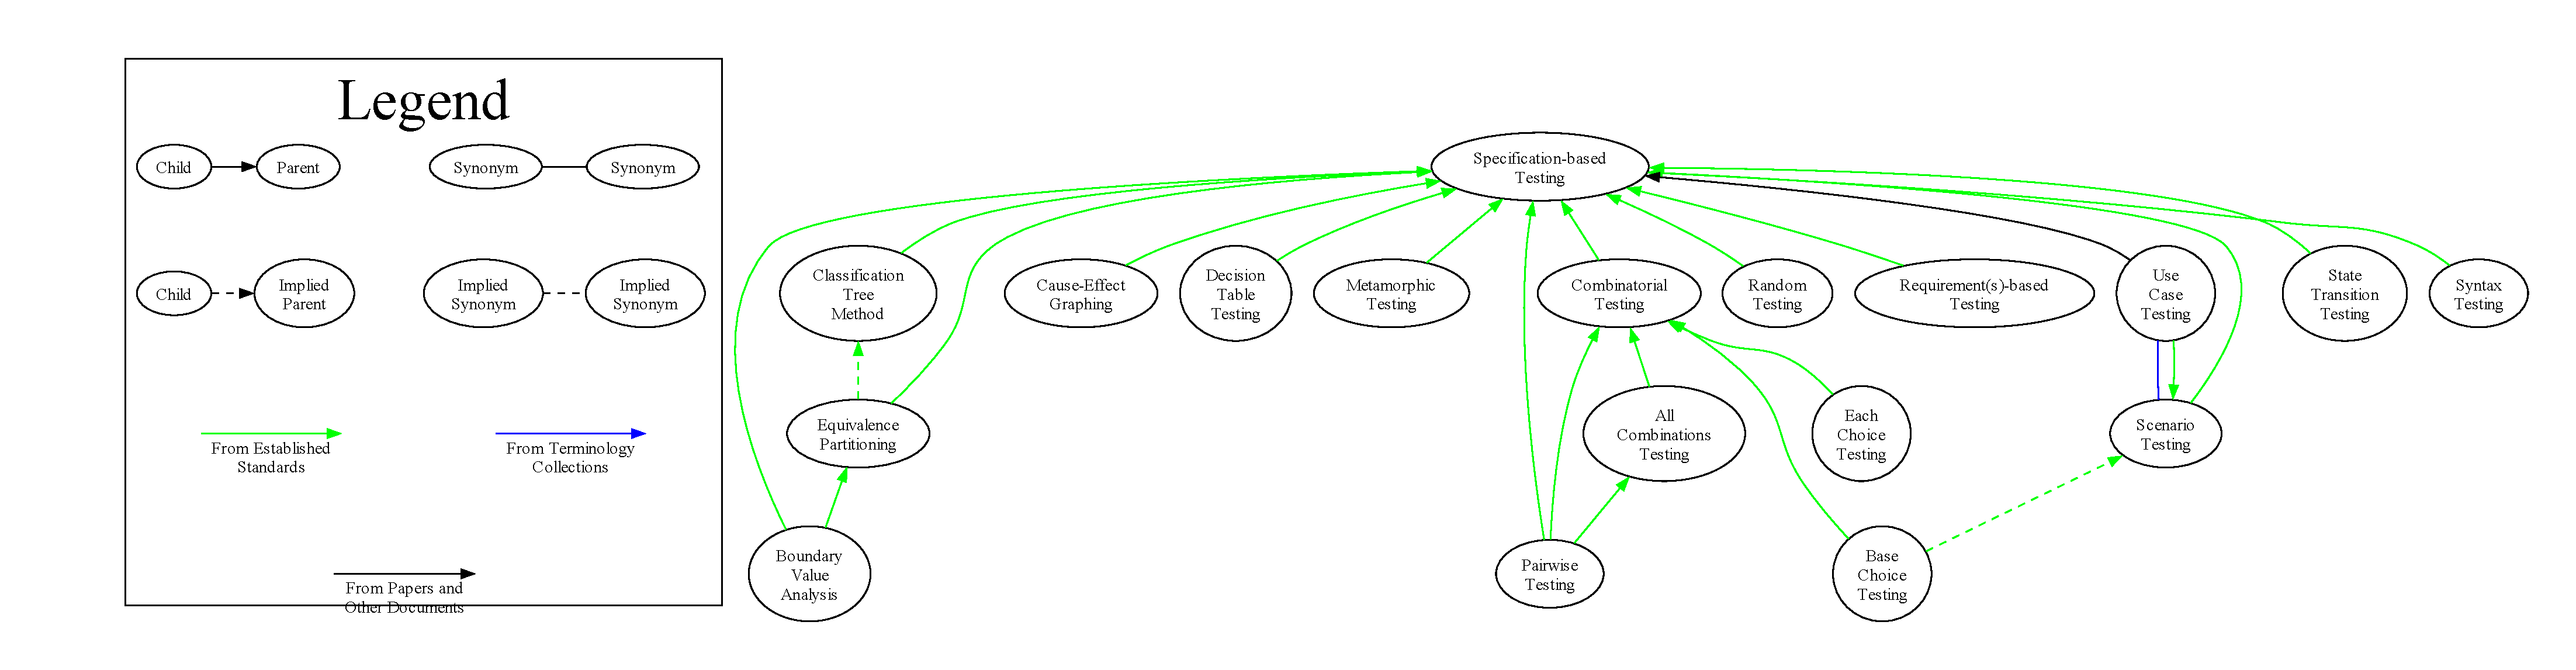
\includegraphics[width=\linewidth]{assets/graphs/specBasedGraph.pdf}
            \caption{``Superset'' relations.}
            \label{fig:specBasedGraph}
        \end{subfigure}
        \begin{subfigure}[t]{.45\linewidth}
            \centering
            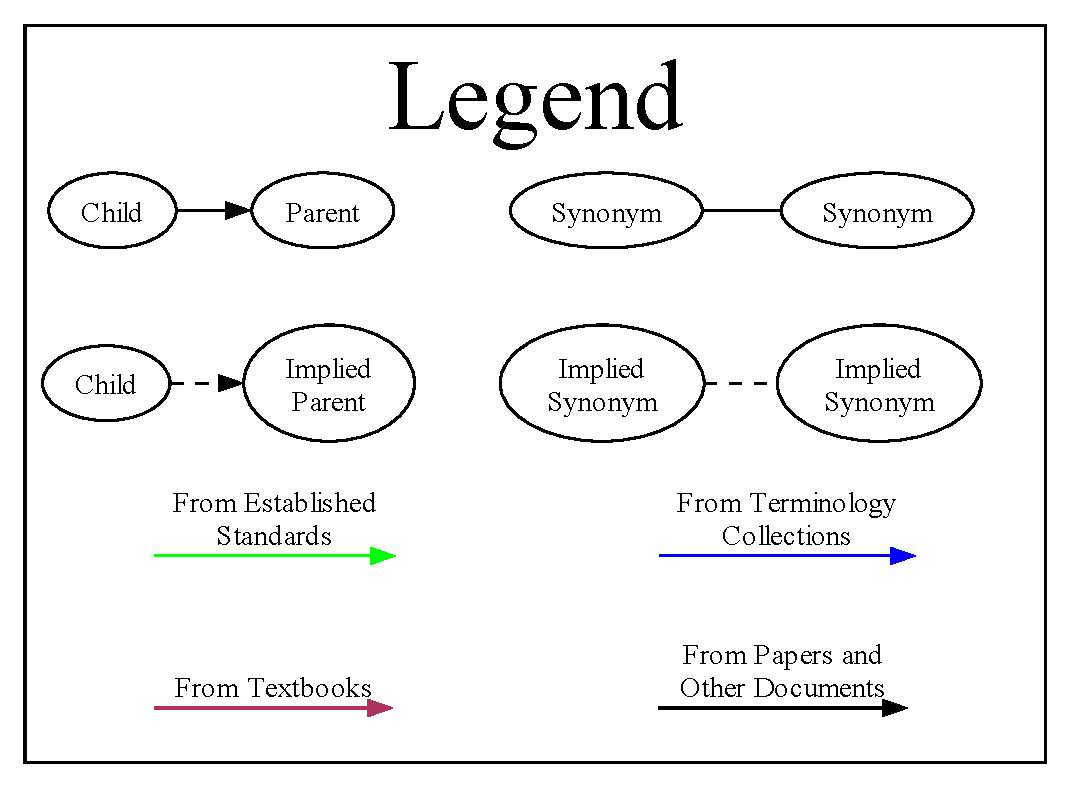
\includegraphics[width=\linewidth]{assets/graphs/parChdLegend.pdf}
        \end{subfigure}
        \begin{subfigure}[t]{.5\linewidth}
            \centering
            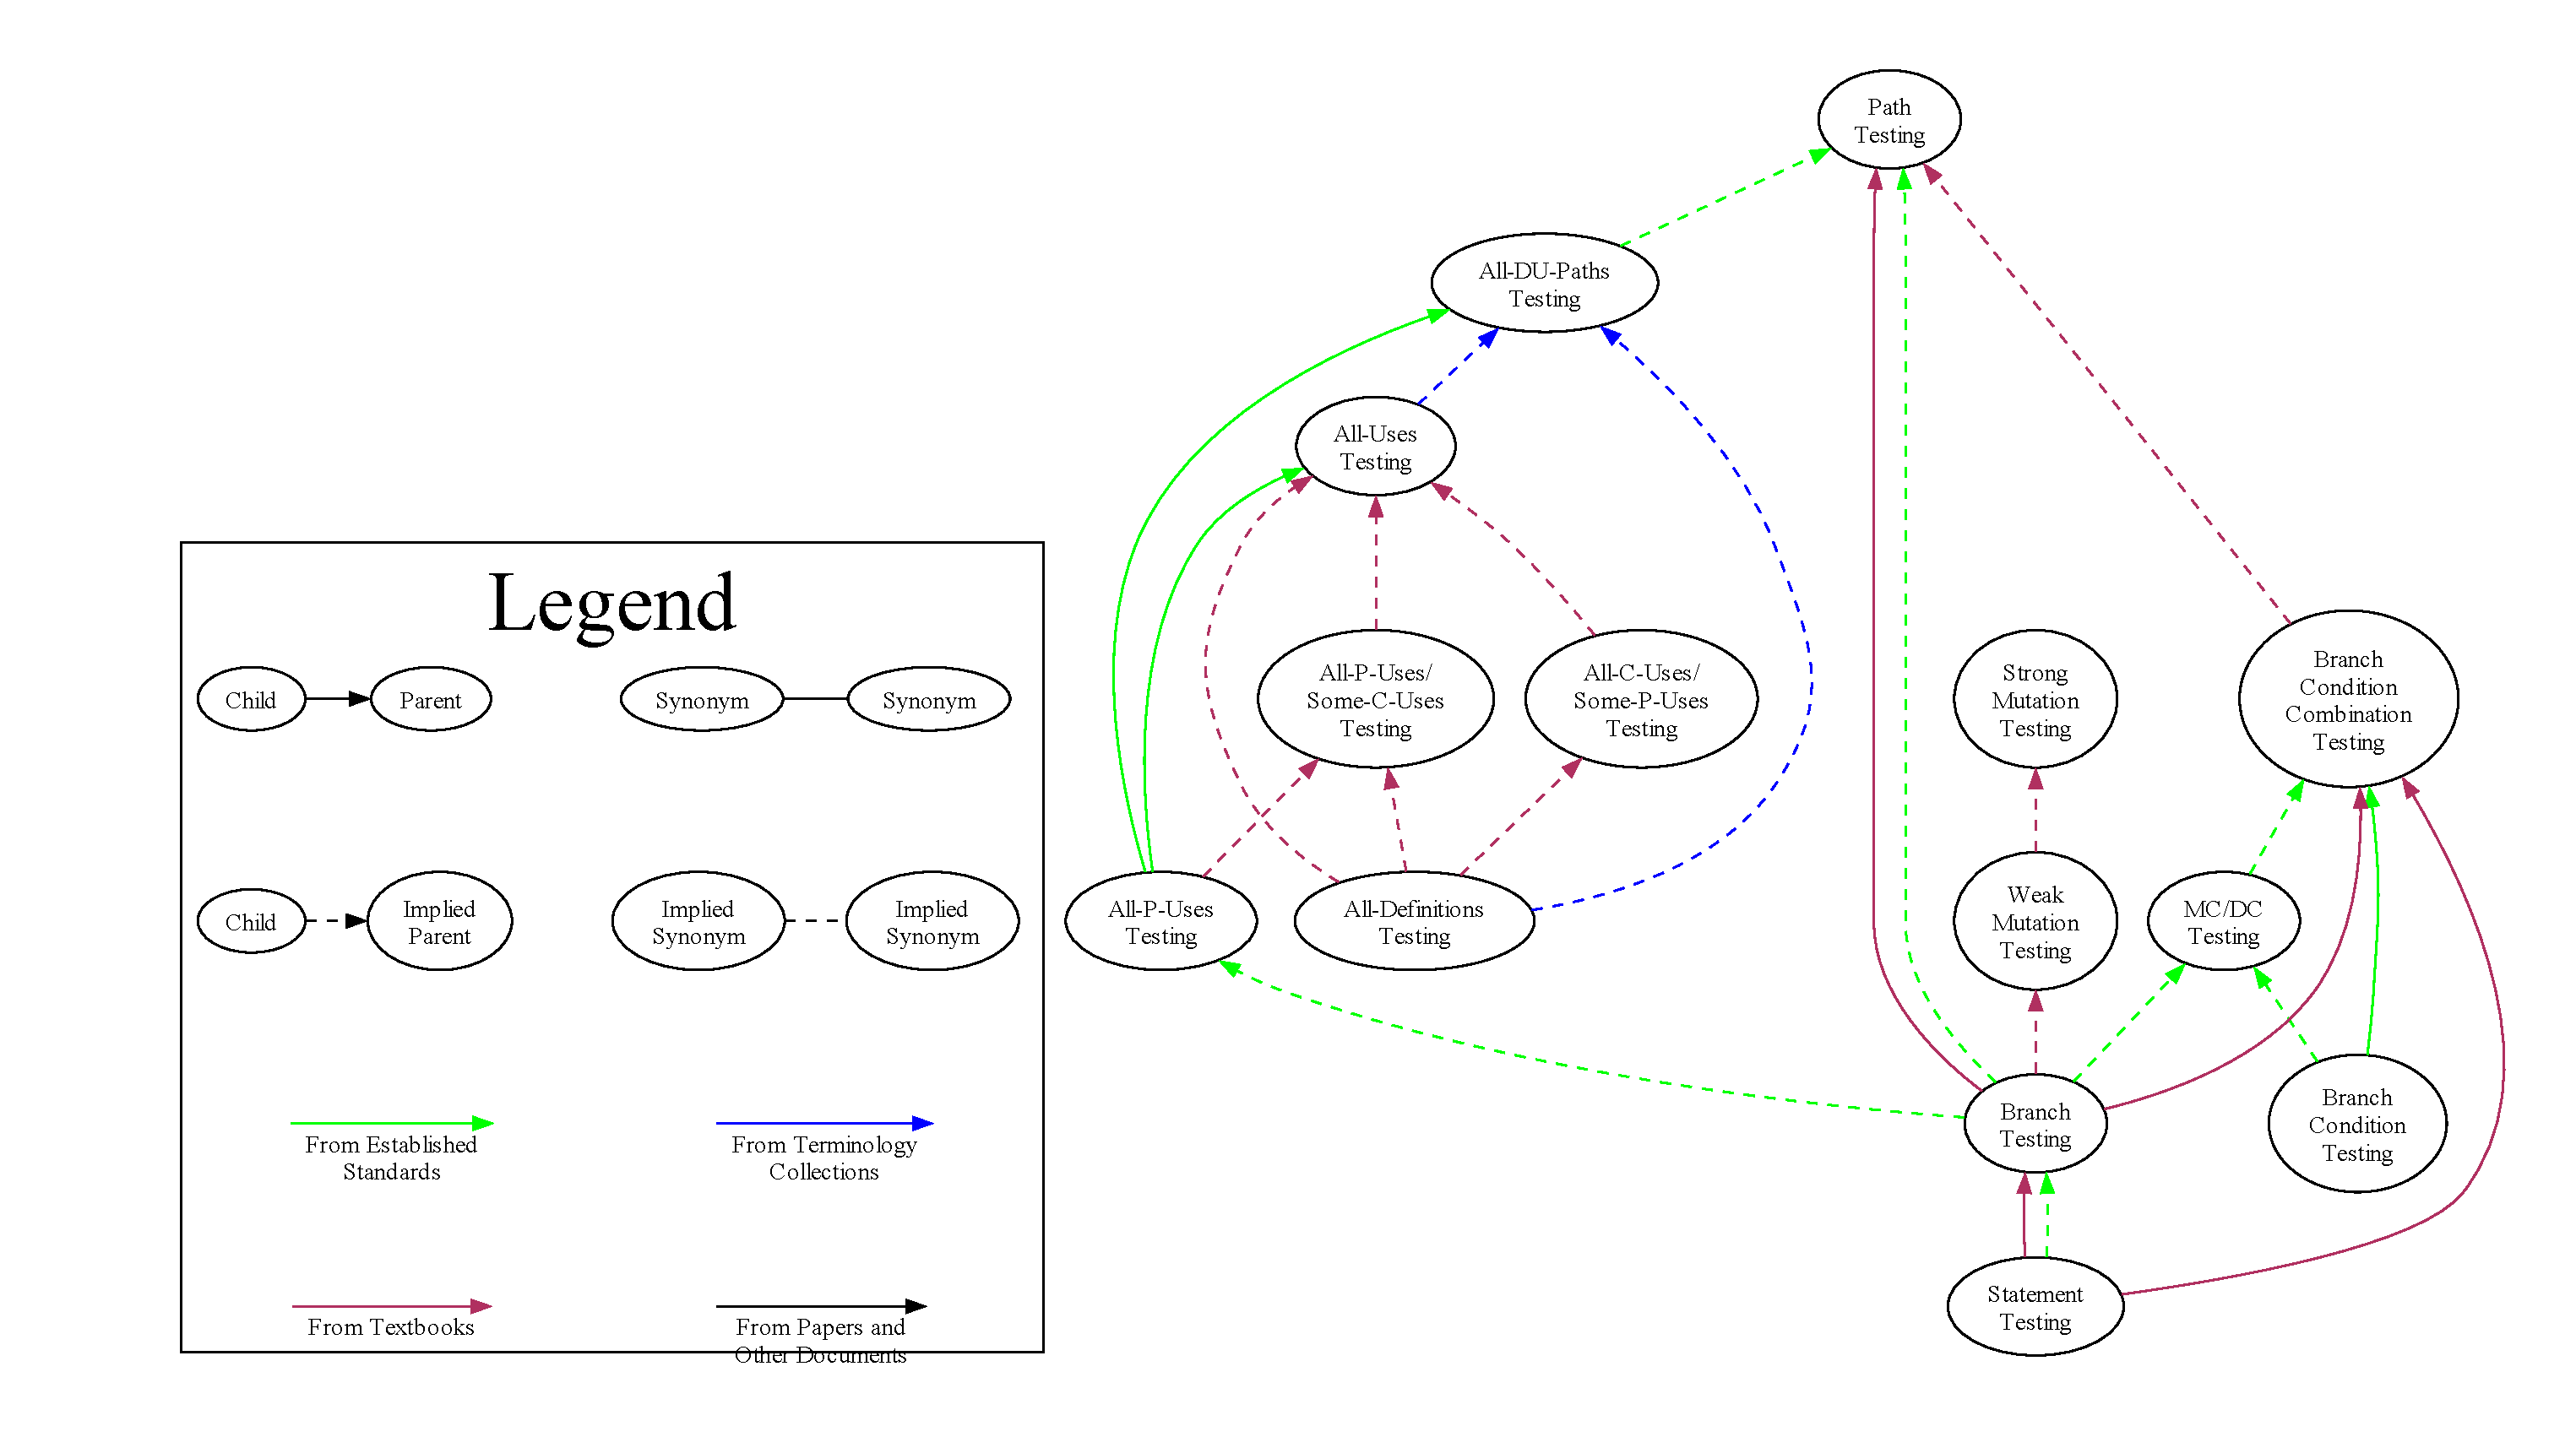
\includegraphics[width=\linewidth]{assets/graphs/subsumesGraph.pdf}
            \caption{``Subsume'' relations.}
            \label{fig:subsumesGraph}
        \end{subfigure}
        \caption{Graphs of different classes of \hyperref[par-chd-rels]{parent-child relations}.}
        \label{fig:parChdGraphs}
    \end{figure}
}

\newcommand{\ExampleGraph}{
    \begin{figure*}
        \begin{subfigure}[b]{0.3\linewidth}
            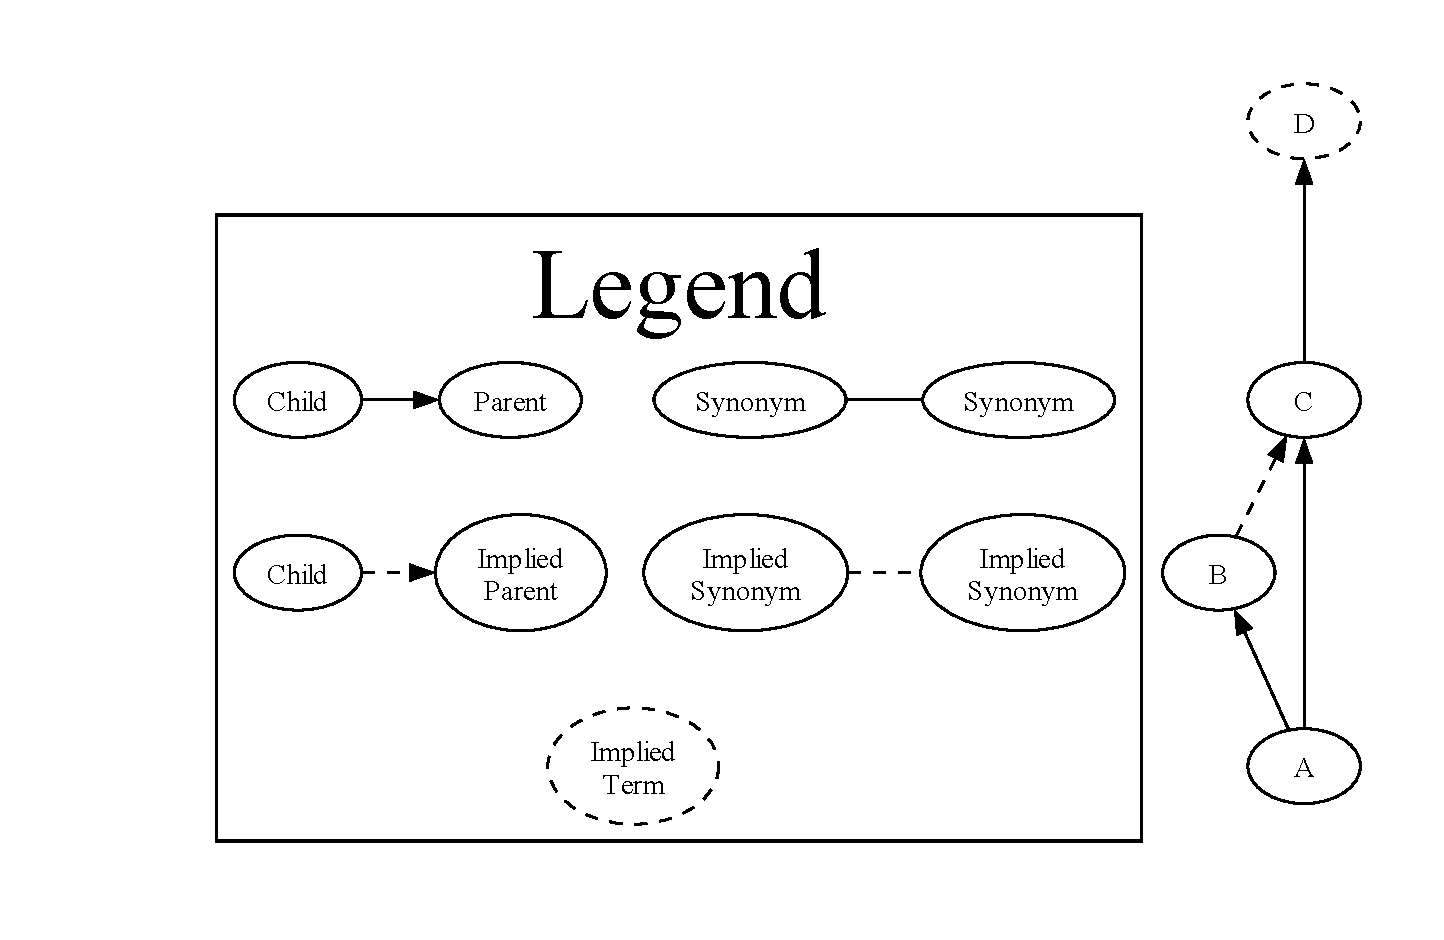
\includegraphics[width=\linewidth]{assets/graphs/ExampleGlossaryGraph.pdf}
            \caption{Graph from \Cref{tab:exampleGlossary}.}
            \label{fig:exampleGraph}
        \end{subfigure}
        \centering
        \begin{subfigure}[b]{0.675\linewidth}
            \centering
            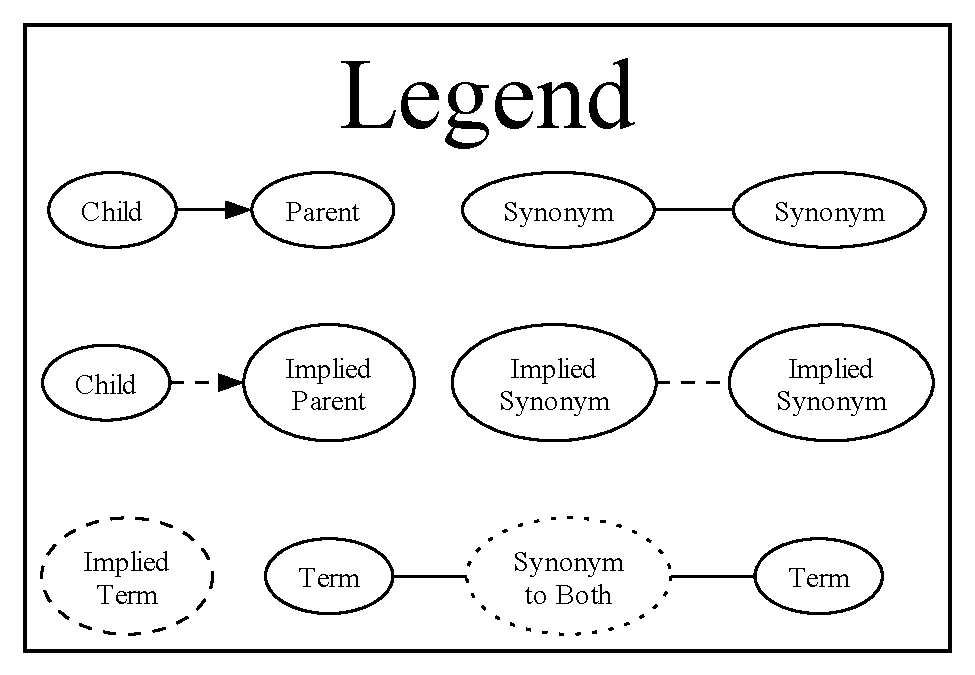
\includegraphics[width=0.8\linewidth]{assets/graphs/manual/manualLegendNonSolidTerms.pdf}
            \hspace{5cm}\begin{subfigure}[t]{0.475\linewidth}
                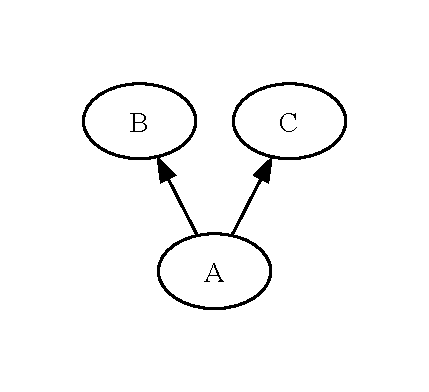
\includegraphics[width=1.1\linewidth]{assets/graphs/rigidExampleGlossaryGraph.pdf}
                \caption{Rigid graph from\\\Cref{tab:exampleGlossary}.}
                \label{fig:rigidExampleGraph}
            \end{subfigure}
            \begin{subfigure}[t]{0.475\linewidth}
                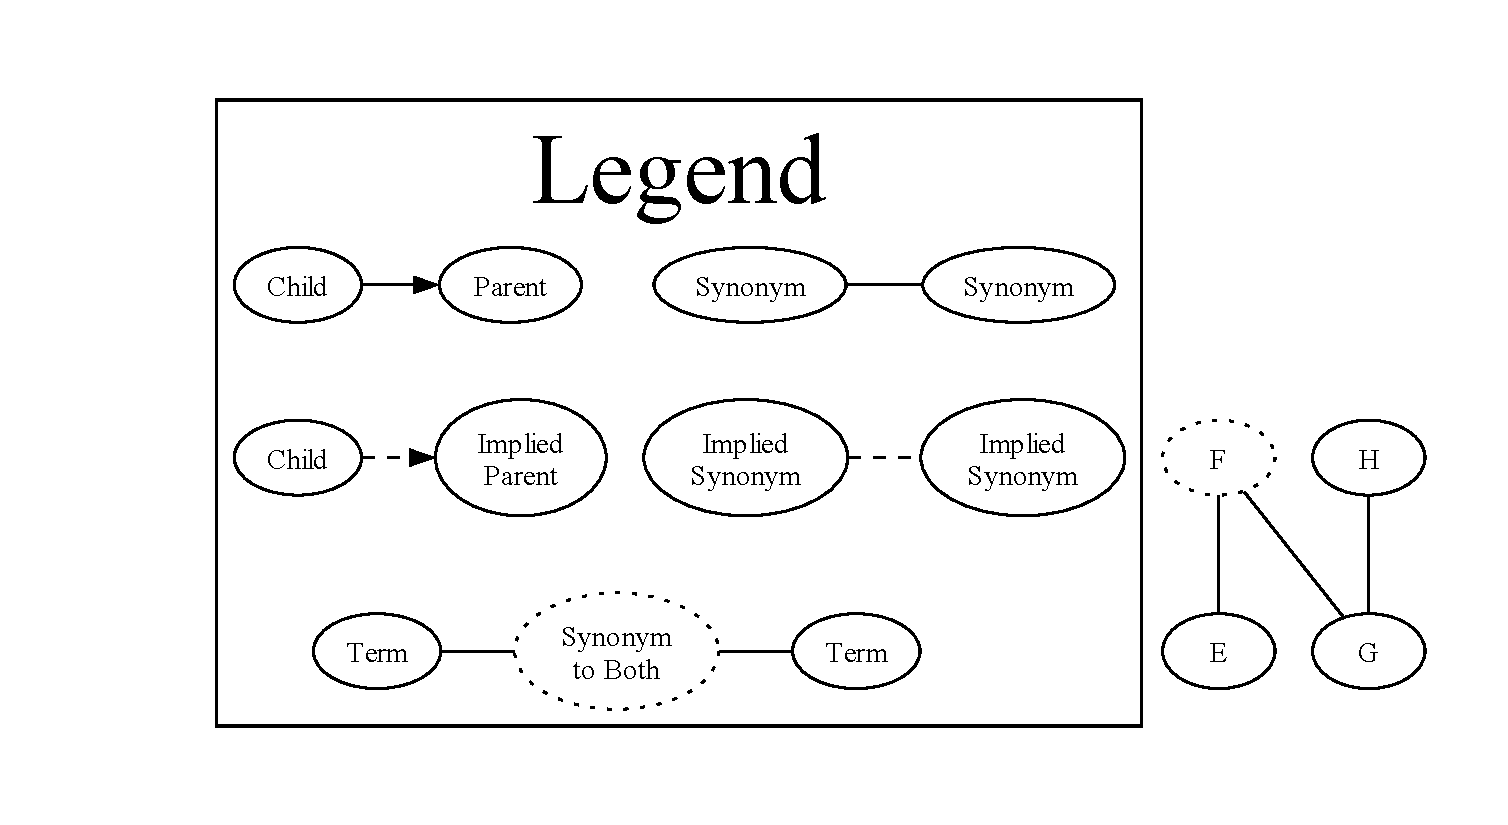
\includegraphics[width=1.1\linewidth]{assets/graphs/SynExampleGlossaryGraph.pdf}
                \caption{Graph from \Cref{tab:synExampleGlossary}.}
                \label{fig:synExampleGraph}
            \end{subfigure}
        \end{subfigure}
        \begin{subfigure}[t]{0.25\linewidth}
            \centering
            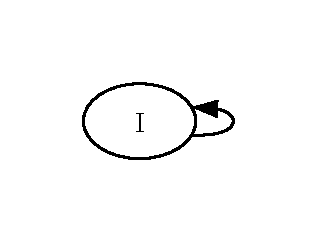
\includegraphics[width=1.2\linewidth]{assets/graphs/SelfExampleGlossaryGraph.pdf}
            \caption{Self-loop graph.}
            \label{fig:selfExampleGraph}
        \end{subfigure}
        \hfill
        \begin{subfigure}[t]{0.425\linewidth}
            \centering
            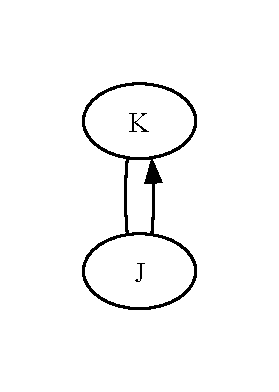
\includegraphics[width=0.6\linewidth]{assets/graphs/ParSynExampleGlossaryGraph.pdf}
            \caption{Graph of a pair of terms with a \hyperref[par-chd-rels]{parent-child} \emph{and} synonym relation.}
            \label{fig:parSynExampleGraph}
        \end{subfigure}
        \hfill
        \begin{subfigure}[t]{0.25\linewidth}
            \centering
            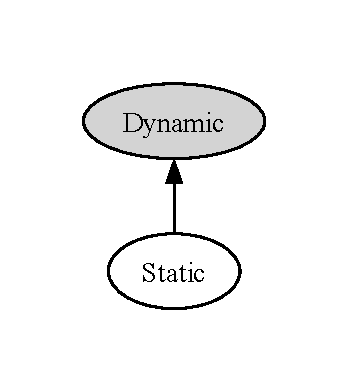
\includegraphics[width=1.4\linewidth]{assets/graphs/StaticExampleGlossaryGraph.pdf}
            \caption{Static graph.}
            \label{fig:staticExampleGraph}
        \end{subfigure}
        \caption{Example generated graphs.}
        \label{fig:exampleGraphs}
    \end{figure*}
}

\newcommand{\recoveryGraphs}{
    % Only top or bottom to comply with IEEE guidelines
    \begin{figure}[bt!]
        \centering
        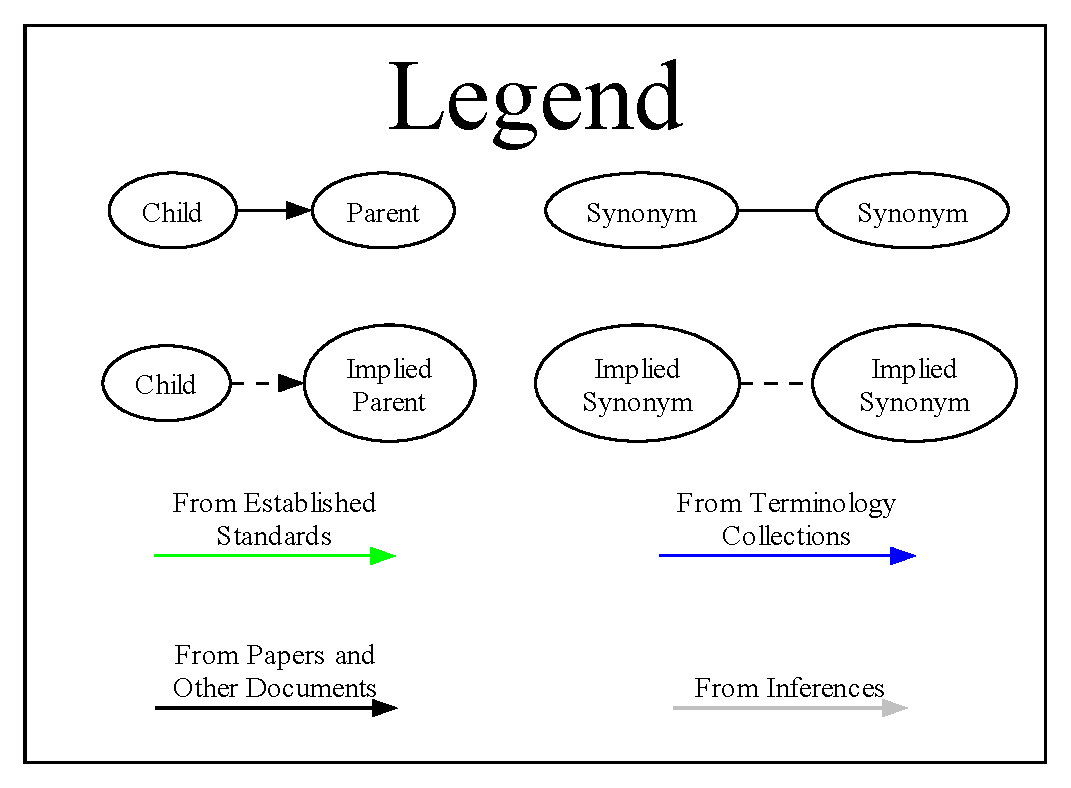
\includegraphics[width=\linewidth]{assets/graphs/recoveryLegend.pdf}
        \begin{subfigure}[b]{.55\linewidth}
            \centering
            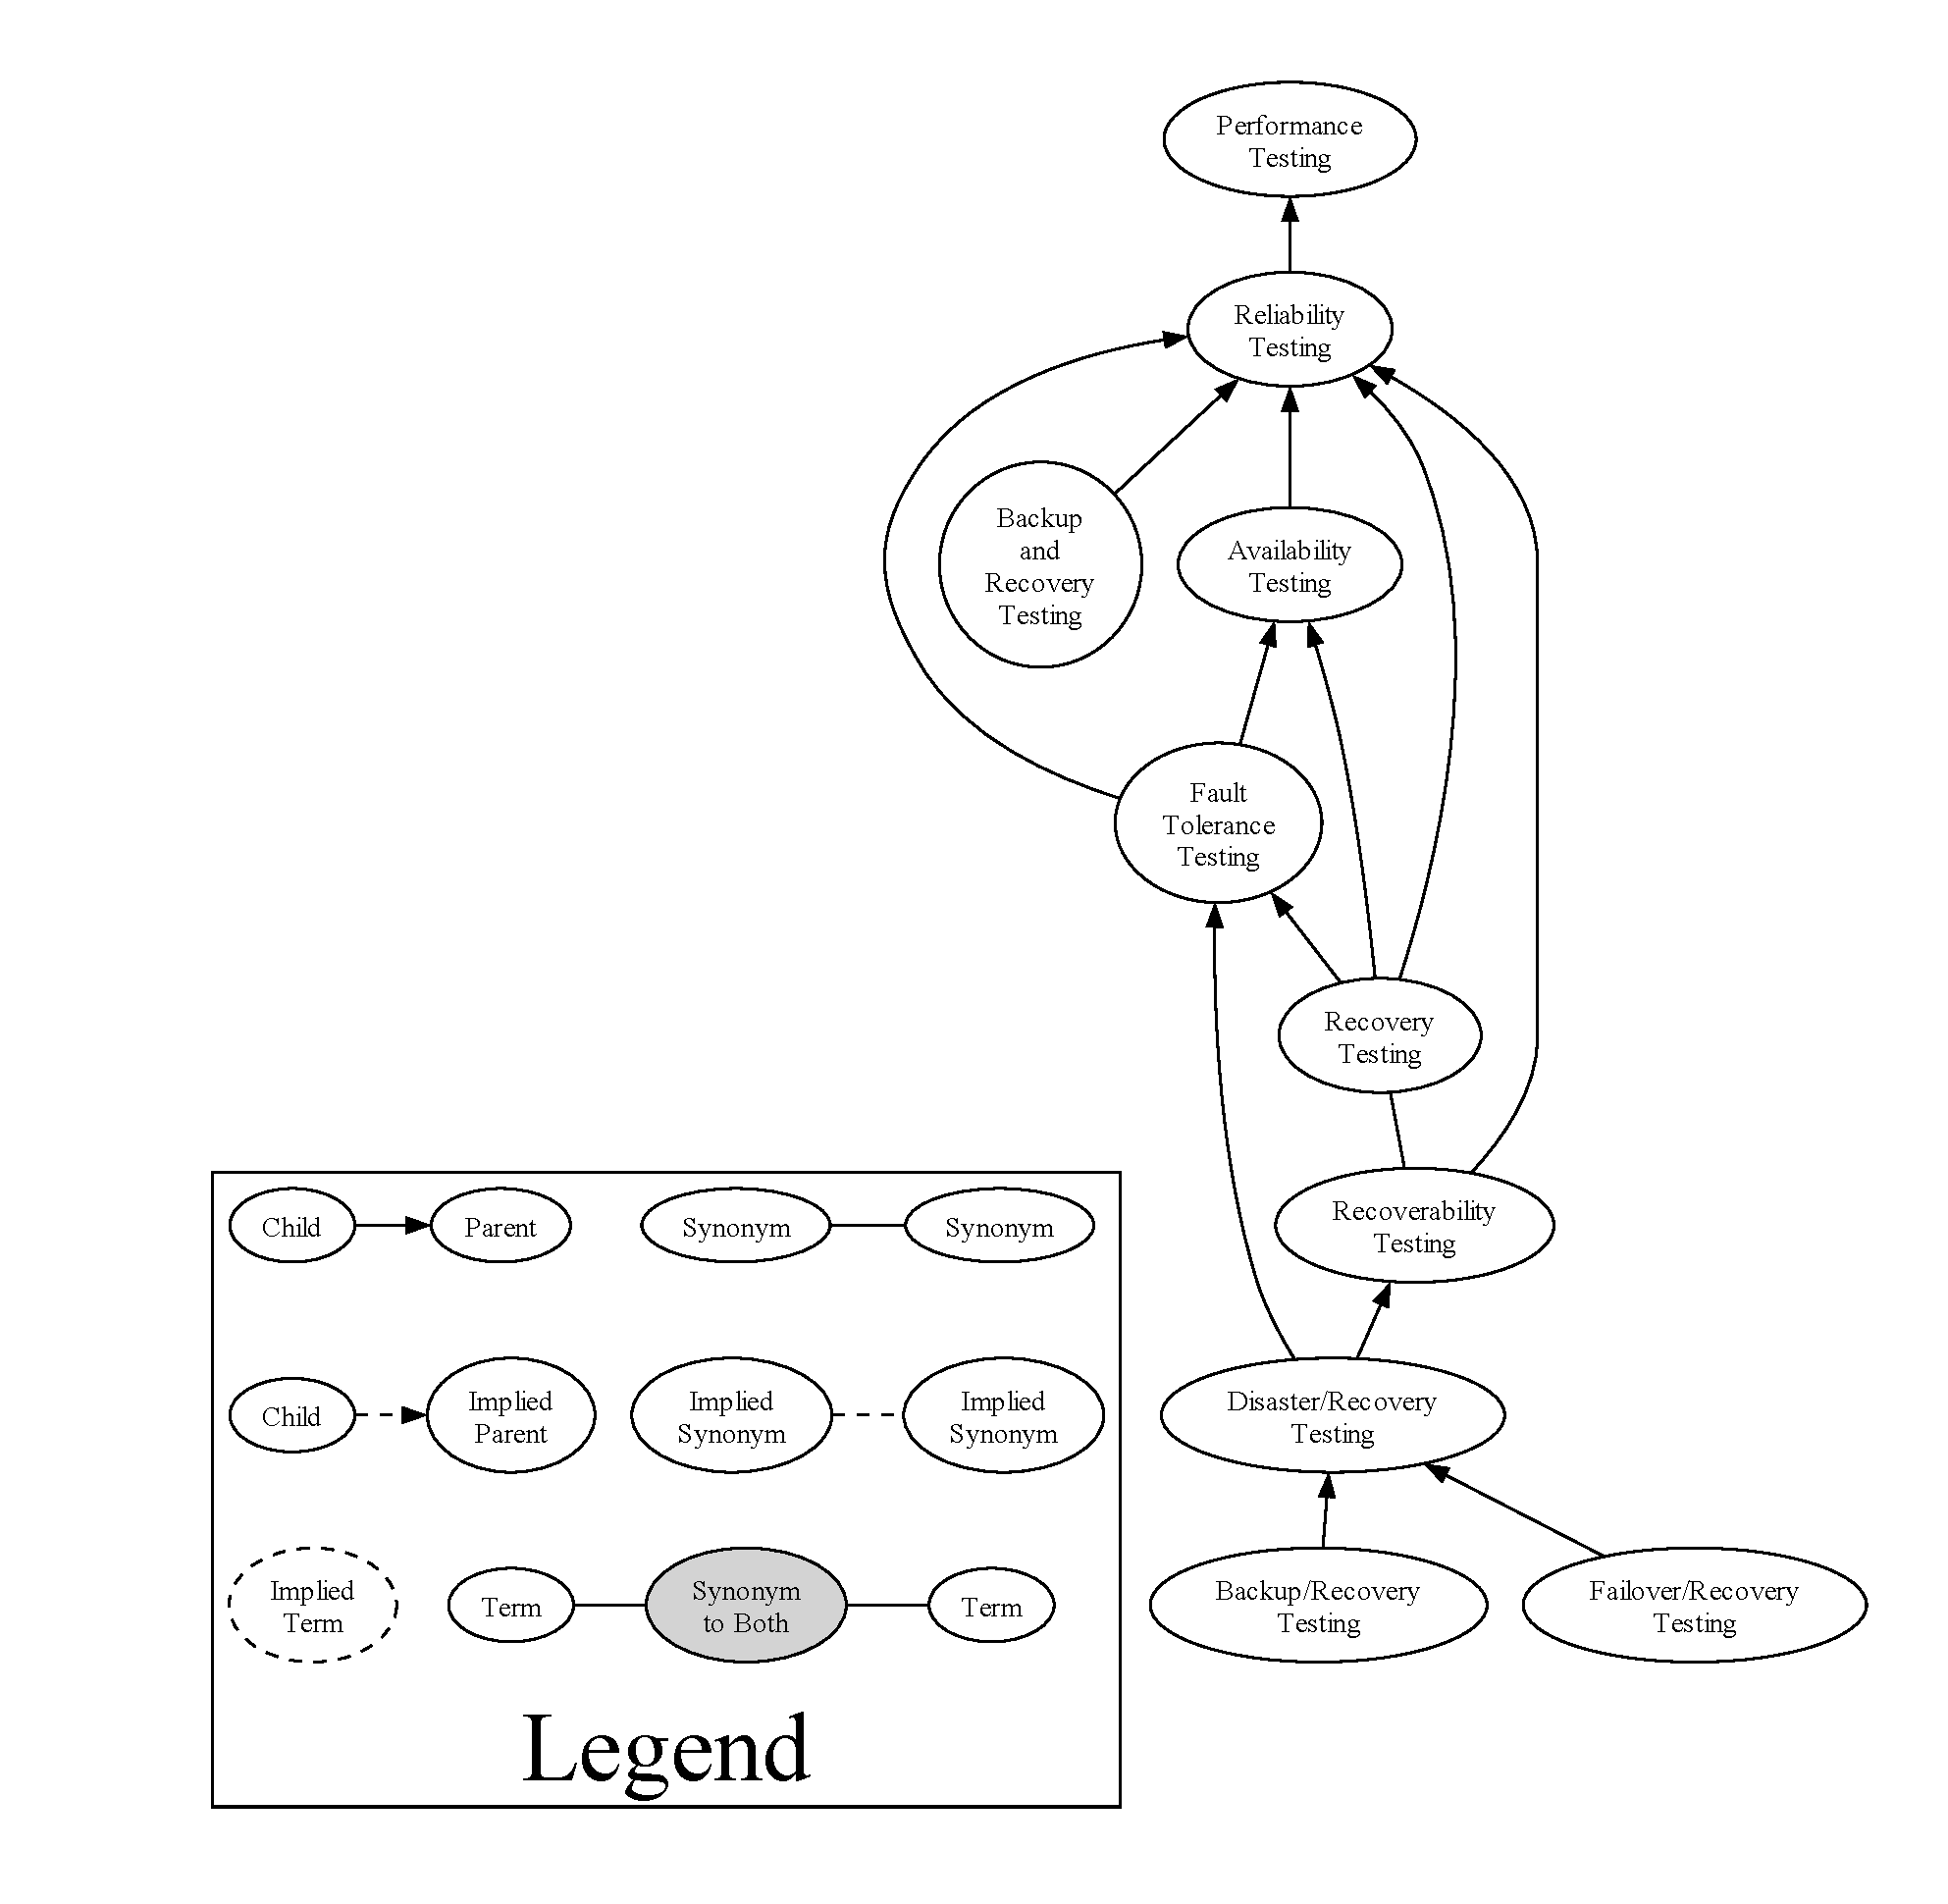
\includegraphics[width=\linewidth]{assets/graphs/recoveryGraph.pdf}
            \caption{Graph of current relations.}
            \label{fig:recovery-graph-current}
        \end{subfigure}
        \begin{subfigure}[b]{.4\linewidth}
            \centering
            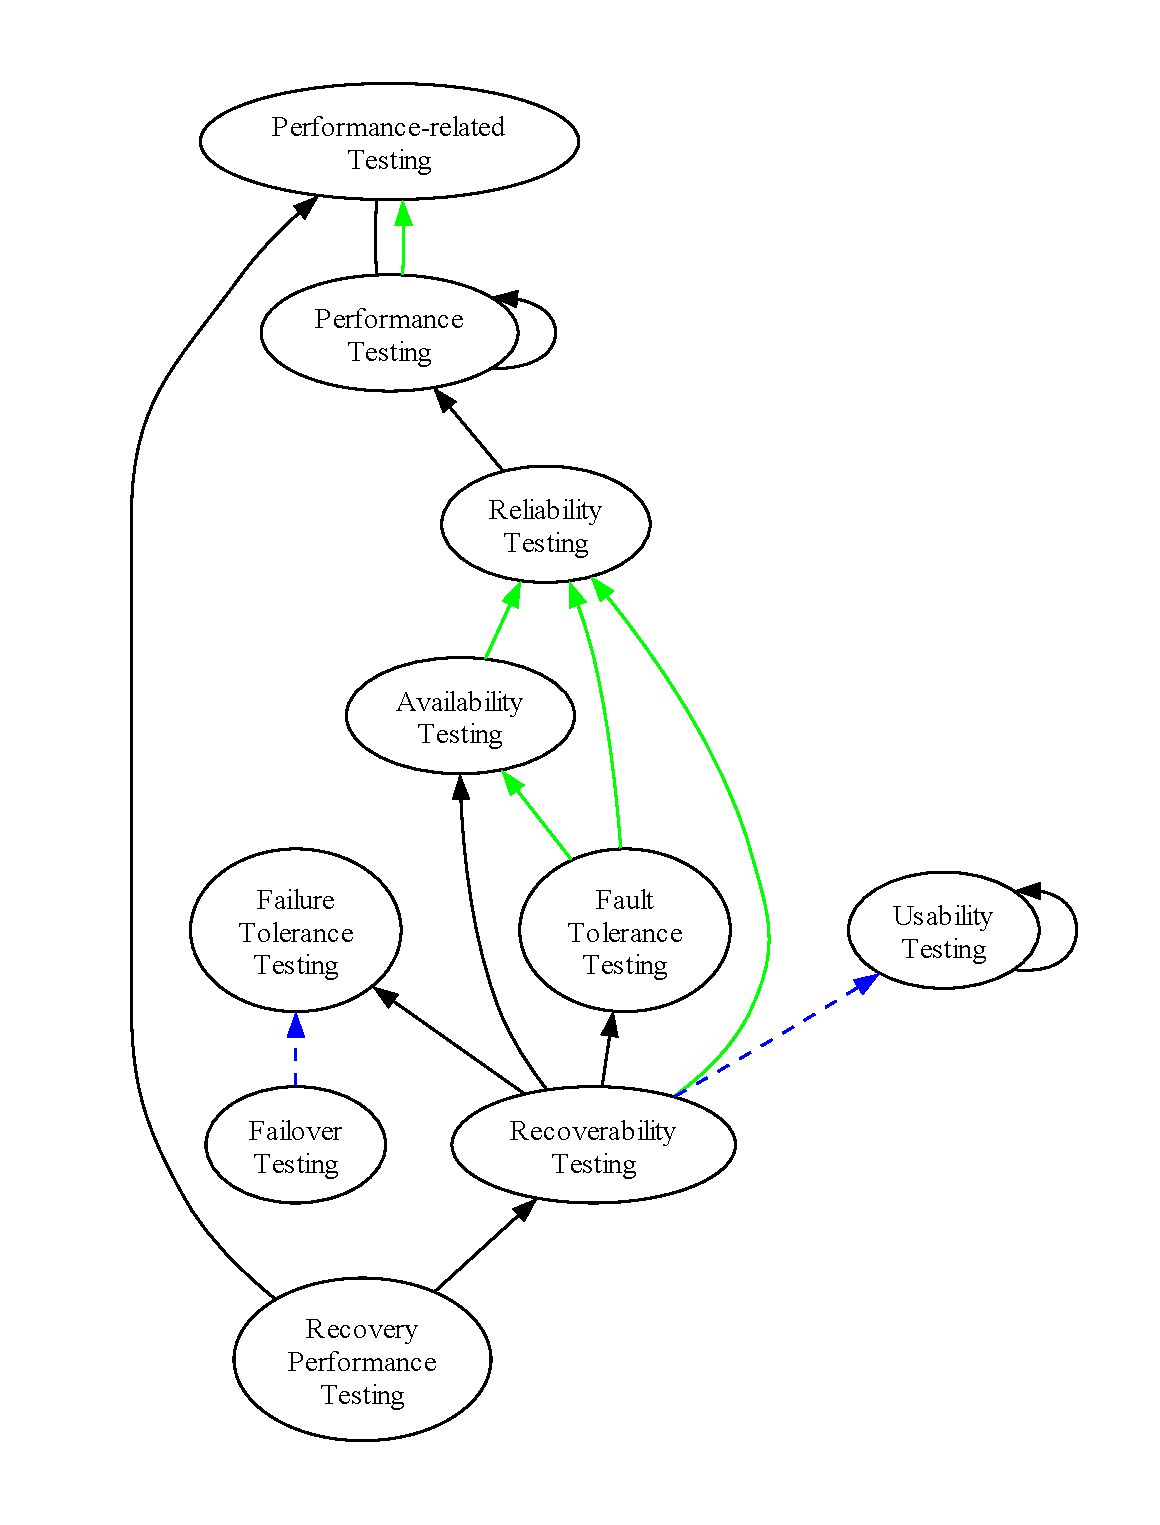
\includegraphics[width=\linewidth]{assets/graphs/recoveryProposedGraph.pdf}
            \caption{Graph of proposed relations.}
            \label{fig:recovery-graph-proposed}
        \end{subfigure}
        \caption{Graphs of relations between terms related to recovery testing.}
        \label{fig:recoveryGraphs}
    \end{figure}
}

\newcommand{\scalGraphs}{
    % Only top or bottom to comply with IEEE guidelines
    \begin{figure}[bt!]
        \centering
        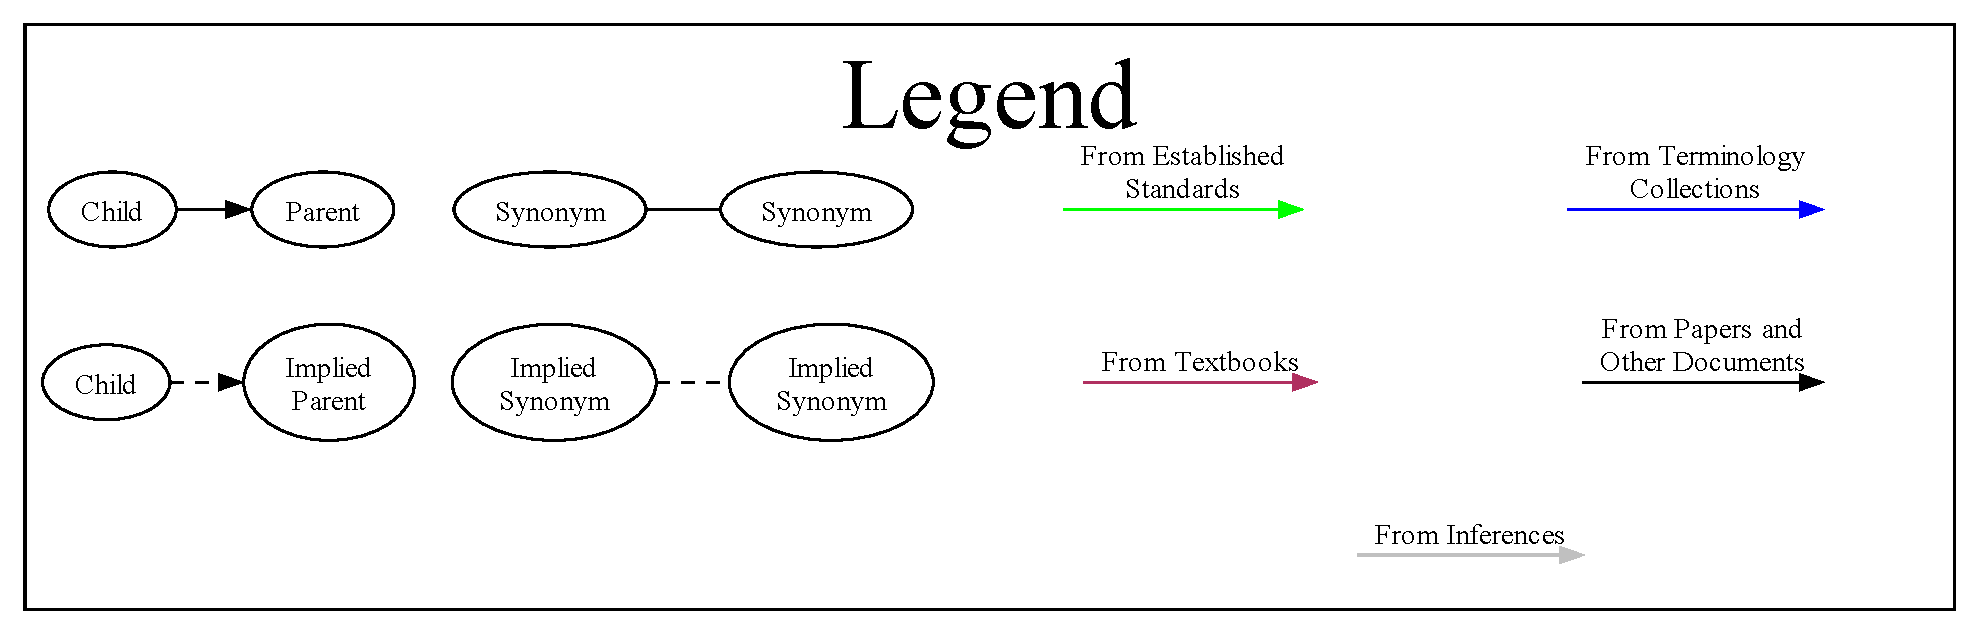
\includegraphics[width=\linewidth]{assets/graphs/scalabilityLegend.pdf}
        \begin{subfigure}[b]{.475\linewidth}
            \centering
            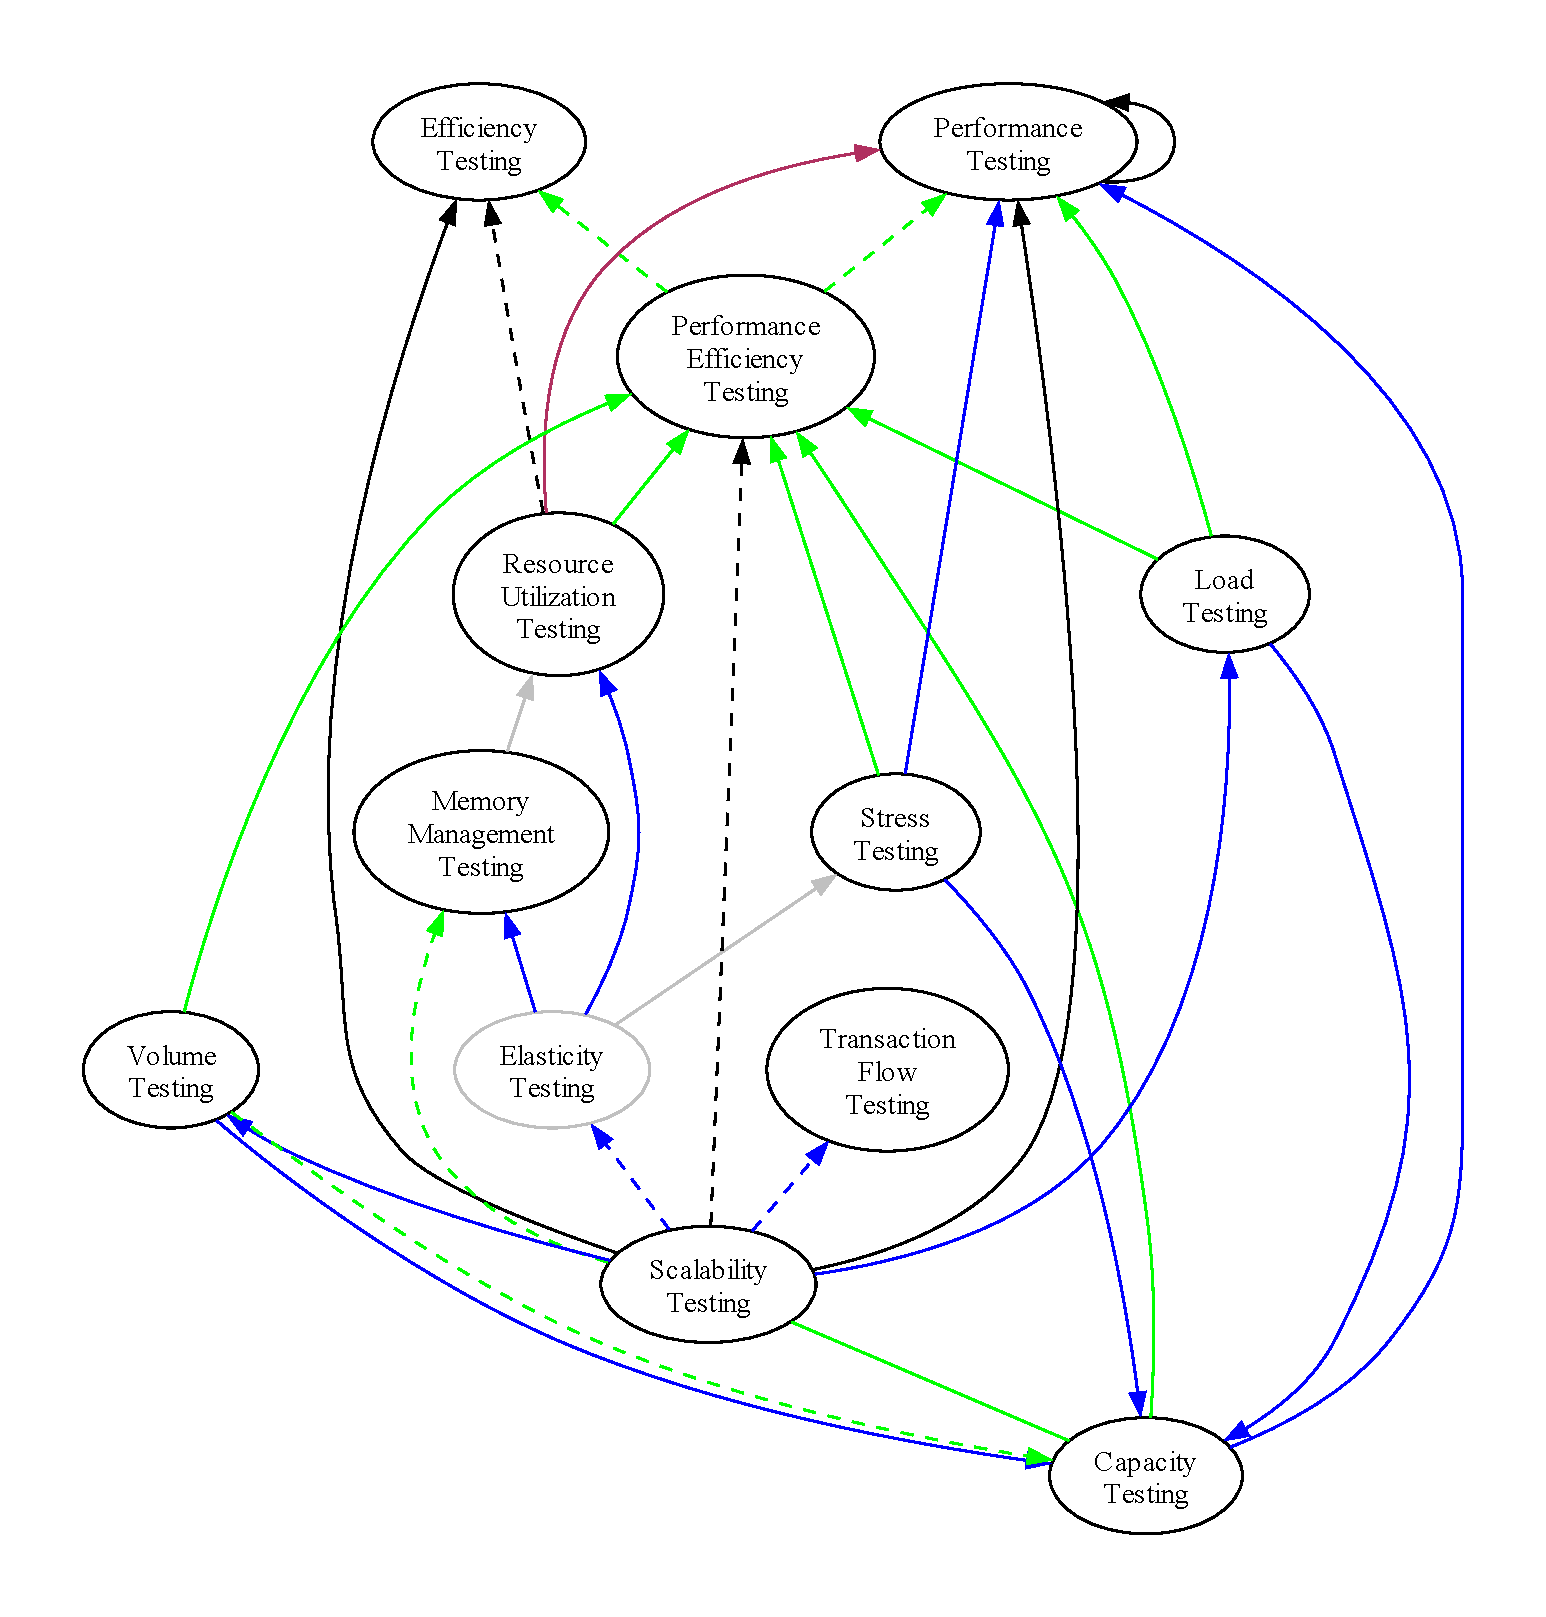
\includegraphics[width=\linewidth]{assets/graphs/scalabilityGraph.pdf}
            \caption{Graph of current relations.}
            \label{fig:scal-graph-current}
        \end{subfigure}
        \begin{subfigure}[b]{.475\linewidth}
            \centering
            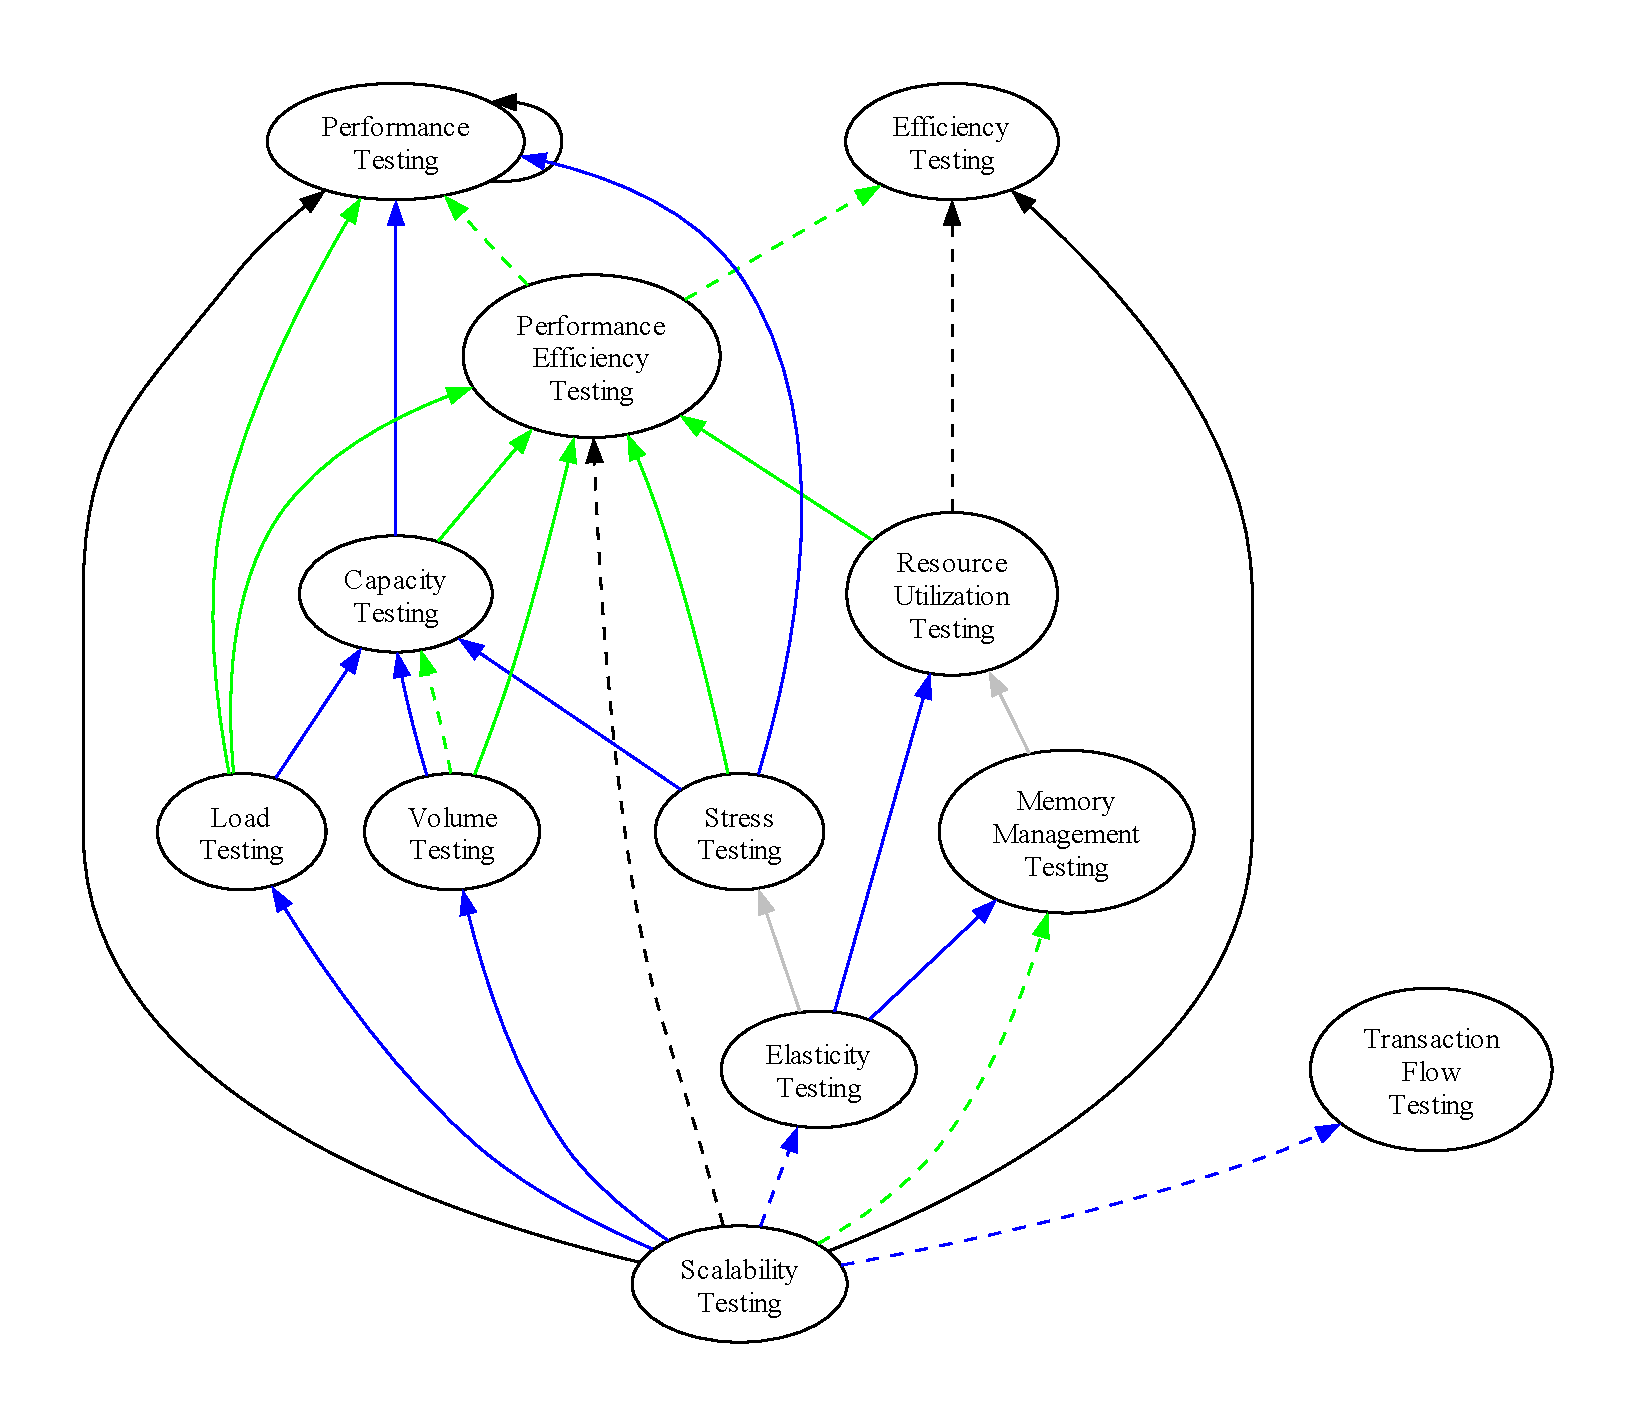
\includegraphics[width=\linewidth]{assets/graphs/scalabilityProposedGraph.pdf}
            \caption{Graph of proposed \ifnotpaper \else \\ \fi relations.}
            \label{fig:scal-graph-proposed}
        \end{subfigure}
        \caption{Graphs of relations between terms related to scalability testing.}
        \label{fig:scalGraphs}
    \end{figure}
}

\newcommand{\performanceGraph}{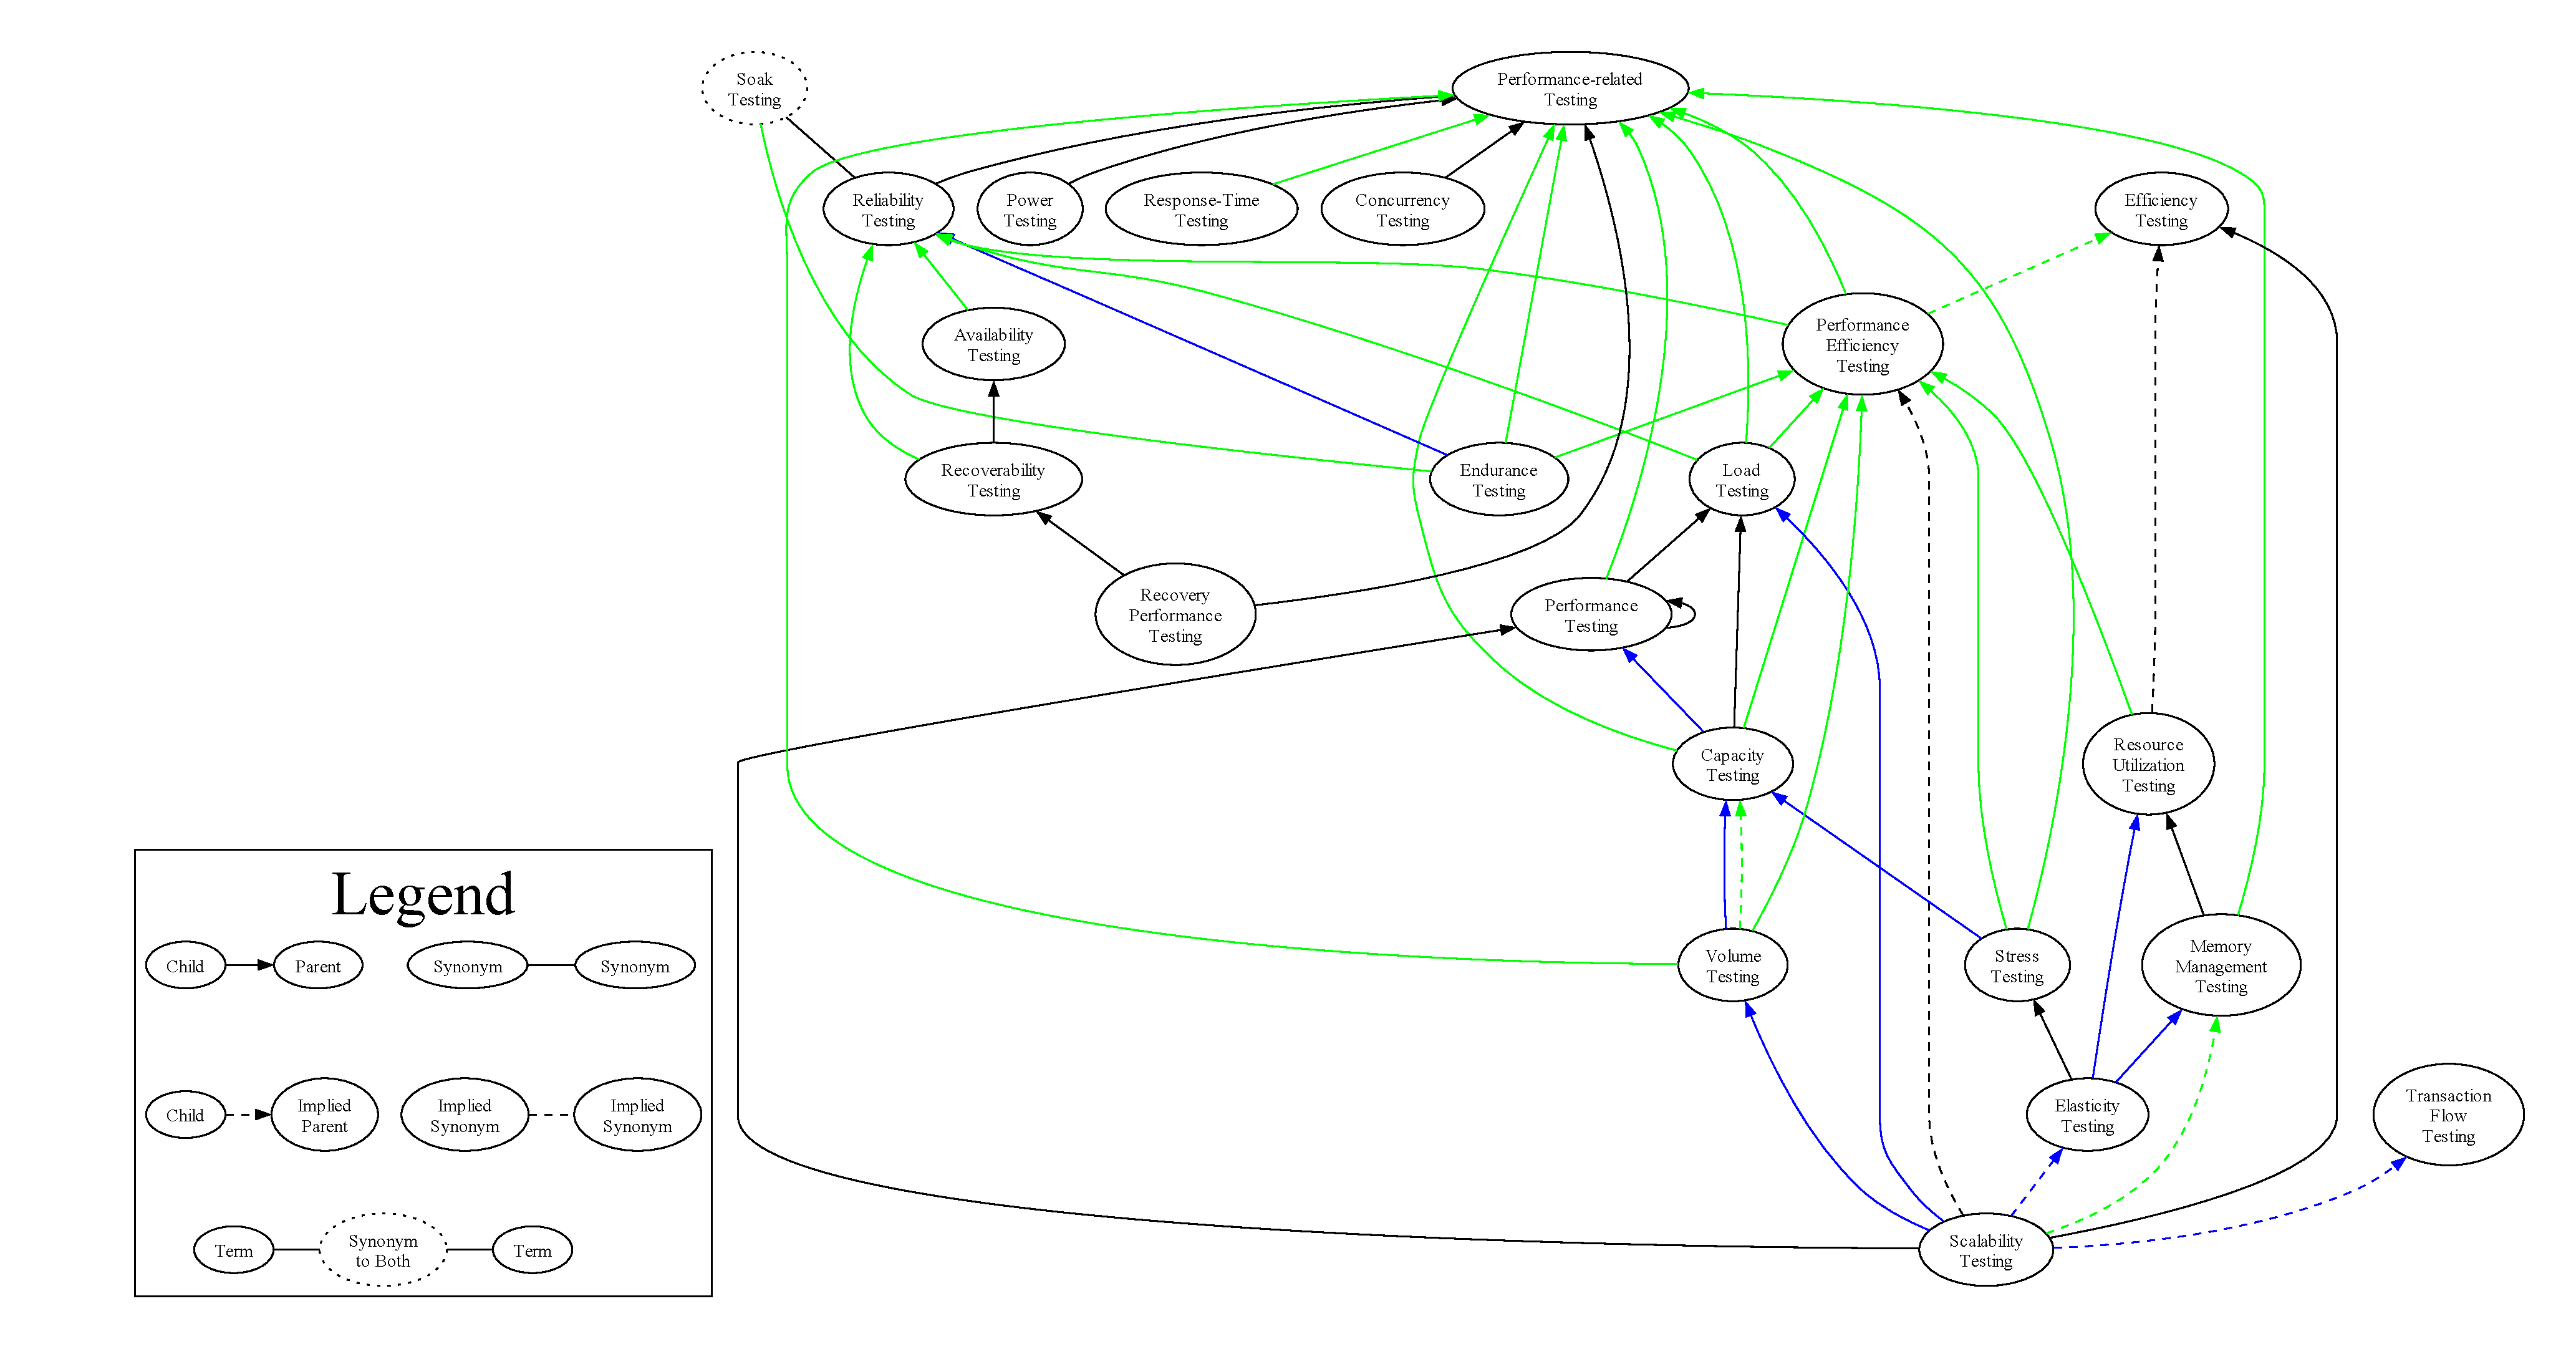
\includegraphics[width=\linewidth]{assets/graphs/performanceProposedGraph.pdf}}

%------------------------------------------------------------------------------
% Images & Figures
%------------------------------------------------------------------------------

\newcommand{\drasilLogo}{assets/images/drasil_logo.png}
\newcommand{\drasilLogoImg}{\begin{figure}[H]
    \centering
    \caption{Drasil's Logo}
    \label{fig:drasilLogo}

    \includegraphics[width=0.6\linewidth]{\drasilLogo}
\end{figure}
}
\newcommand{\refDrasilLogoImg}{\Cref{fig:drasilLogo}}

%------------------------------------------------------------------------------
% Tables
%------------------------------------------------------------------------------

% Organization of files
\newcommand{\organizationTable}{\begin{longtable}[c]{|>{\raggedright}p{0.3\linewidth}|>{\raggedright\arraybackslash}p{0.54\linewidth}|}
    \caption{Template Organization}
    \label{tab:organization}                                              \\

    \hline

    \rowcolor{McMasterMediumGrey}
    \textbf{File/Folder}     & \textbf{Intended Usage \& Description}
    \\ \hline

    \texttt{thesis.tex} & Focal \LaTeX{} file that collects everything and is
    used to build your thesis/report document.
    \\ \hline

    \texttt{Makefile} & A basic \texttt{Makefile} configuration. See
    \texttt{make help} for a list of helpful commands. \\ \hline

    \texttt{build/} & When you build your \acs{pdf}, this folder is used as the
    working directory of LuaLaTeX. Using this allows us to quickly get rid of
    \LaTeX{} build files that can cause problems when we re-build documents. \\
    \hline

    \texttt{manifest.tex} & Basic options that you should certainly configure
    according to your needs.
    \\ \hline

    \texttt{chapters.tex} & All chapters of your thesis should be included here.
    \\ \hline

    \texttt{chapters/} & Enumeration of the chapters of your thesis. I prefer
    using a two-digit indexing pattern for the prefix of file names so that I
    can quickly open up by chapter number using VS Codium. \\ \hline

    \texttt{assets.tex} & Enumeration of the various kinds of ``assets'' in the
    \texttt{assets/} folder. See the file for examples on how you can write your
    extra utility macros. \\ \hline

    \texttt{assets/} & Enumeration of various kinds of ``assets,'' with
    subdirectories for images and figures, tables, and code snippets. \\ \hline

    \texttt{front.tex} & All front matter of your thesis should be included
    here. \\ \hline

    \texttt{front/} & Enumeration of the front chapters of your thesis. These
    chapters should all be numbered using Roman numerals. \\ \hline

    \texttt{back.tex} & All back matter of your thesis should be included here.
    \\ \hline

    \texttt{back/} & Enumeration of the back matter content.
    \\ \hline

    \texttt{acronyms.tex} & List of acronyms you intend to use in your thesis.
    This uses the ``acro'' \LaTeX{} package.
    \\ \hline

    \texttt{macros.tex} & Helpful macros!
    \\ \hline

    \texttt{unicode\_chars.tex} & At times, you might find issues with unicode
    characters, especially in verbatim environments, where you might need to
    manually define them using other font glyphs.
    \\ \hline

    \texttt{mcmaster\_colours.tex} & Macros for the McMaster colour palette.
    \\ \hline

    \texttt{README.md} & Read it!
    \\ \hline

    \texttt{.gitignore} & List of files in the working directory that should be
    ignored by git.
    \\ \hline

    \texttt{latexmkrc} & Used for setting the timezone for latexmk, but can be
    used for other options.
    \\ \hline
\end{longtable}
}

\newcommand{\ieeeCatsTable}{% Conversion to longtblr assisted by GitHub Copilot

\begin{longtblr}[
    note{a} = {Also called ``test phase'' \ifnotpaper (see
            \discrepref{level-phase-syns}) \fi or ``test stage'' \ifnotpaper
            (see \discrepref{stage-level-syns})\else (see relevant synonym
            discrepancies in \Cref{syns})\fi.},
    note{b} = {Also called ``test design technique'' \ifnotpaper
            (\citealp[p.~11]{IEEE2022}; \citealpISTQB{})\else
            \cite[p.~11]{IEEE2022}, \cite{ISTQB}\fi.},
    caption={Categories of testing given by ISO/IEC and IEEE.},
    label={tab:ieeeCats}
    ]{
    colspec={|X[0.09,c,m]X[0.56,m]X[0.3,m]|},
    width = \linewidth, rowhead = 1, hlines
    }
    \thead{Term}                   & \thead{Definition}                           & \thead{Examples} \\
    Test Approach                  & A ``high-level test implementation choice''
    that includes ``test level, test type, test technique, test practice and
    \dots{} static testing'' \citep[p.~10]{IEEE2022} and is used to ``pick the
    particular test case values''
    \citeyearpar[p.~465]{IEEE2017} & black or white box, minimum and maximum
    boundary value testing \citep[p.~465]{IEEE2017}                                                  \\

    Test Level\TblrNote{a}         & A stage of testing ``typically associated
    with the achievement of particular objectives and used to treat particular
    risks'', each performed in sequence \ifnotpaper (\citealp[p.~12]{IEEE2022};
    \citeyear[p.~6]{IEEE2021}) \else \cite[p.~12]{IEEE2022}, \cite[p.~6]{IEEE2021}
    \fi with their ``own documentation and resources''
    \citeyearpar[p.~469]{IEEE2017} % ; more generally, ``designat[es] \dots\ the
    % coverage and detail'' \citeyearpar[p.~249]{IEEE2017} 
                                   & unit/component testing, integration testing,
    system testing, acceptance testing \ifnotpaper (\citealp[p.~12]{IEEE2022};
    \citeyear[p.~6]{IEEE2021}; \citeyear[p.~467]{IEEE2017}) \else
    \cite[p.~12]{IEEE2022}, \cite[p.~467]{IEEE2017}, \cite[p.~6]{IEEE2021} \fi                       \\
    Test Practice                  & A ``conceptual framework that can be
    applied to \dots{} [a] test process to facilitate testing'' \ifnotpaper
    (\citealp[p.~14]{IEEE2022}; \citeyear[p.~471]{IEEE2017}; OG IEEE 2013)
    \else \cite[p.~14]{IEEE2022}, \cite[p.~471]{IEEE2017}
    \fi % ; more generally, a ``specific type of activity that contributes to
    % the execution of a process'' \citeyearpar[p.~331]{IEEE2017} 
                                   & scripted testing, exploratory testing,
    automated testing \citep[p.~20]{IEEE2022}                                                        \\
    Test Technique\TblrNote{b}     & A ``procedure used to create or select a
    test model, identify test coverage items, and derive corresponding test
    cases'' \ifnotpaper (\citeyear[p.~11]{IEEE2022}; similar in
    \citeyear[p.~467]{IEEE2017}) \else \cite[p.~11]{IEEE2022} (similar in
    \cite[p.~467]{IEEE2017}) \fi that ``generate evidence that test item
    requirements have been met or that defects are present in a test item''
    \citeyearpar[p.~vii]{IEEE2021} % ; ``a variety \dots\ is typically
    % required to suitably cover any system'' \citeyearpar[p.~33]{IEEE2022} and
    % is ``often selected based on team skills and familiarity, on the format
    % of the test basis'', and on expectations \citeyearpar[p.~23]{IEEE2022}
                                   & equivalence partitioning,
    boundary value analysis, branch testing \citep[p.~11]{IEEE2022}                                  \\
    Test Type                      & ``Testing that is focused on specific
    quality characteristics'' \ifnotpaper (\citealp[p.~15]{IEEE2022};
    \citeyear[p.~7]{IEEE2021}; \citeyear[p.~473]{IEEE2017}; OG IEEE 2013)
    \else \cite[p.~15]{IEEE2022}, \cite[p.~473]{IEEE2017}, \cite[p.~7]{IEEE2021}
    \fi                            & security testing, usability testing,
    performance testing \ifnotpaper (\citealp[p.~15]{IEEE2022};
    \citeyear[p.~473]{IEEE2017}) \else\cite[p.~15]{IEEE2022},
    \cite[p.~473]{IEEE2017} \fi                                                                      \\
\end{longtblr}
}
\newcommand{\otherCatsTable}{% Defined here so VS Code doesn't freak out
\def\ieeeEquiv{\makecell{IEEE\\Equivalent}}
\def\swebokLevel{{Level\\(objective-\\based)\TblrNote{a}}}

\begin{longtblr}[
    note{a} = {See \flawref{stage-level-syns}.},
    note{b} = {Testing methods and guidances are omitted from this table
            since \citet{BarbosaEtAl2006} do not define or give examples of them.},
    note{c} = {Synonyms for these examples are used by
            \citet[p.~3; OG Mathur, 2012]{SouzaEtAl2017} and
            \citet[p.~3]{BarbosaEtAl2006}.},
    caption={Categories of testing given by other sources.},
    label={tab:otherCats}
    ]{
    colspec={|X[0.08,c,m]|X[0.43,m]|X[0.34,m]|Q[c,m]|},
    width = \linewidth, rowhead = 1
    }
    \hline
    \thead{Term}                           & \thead{Definition}           & \thead{Examples} & \thead{\ieeeEquiv{}} \\
    \hline
    % Guidance                               & none given
    % \citep[p.~3]{BarbosaEtAl2006}          & none given         & Technique?                              \\
    \swebokLevel{}                         & Test levels based on the
    purpose of testing \citep[p.~5\=/6]{SWEBOK2024} that ``determine
    how the test suite is identified \dots\ regarding its consistency
    \dots\ and its composition''
    \citetext{p.~5\=/2}                    & conformance testing,
    installation testing, regression testing, performance testing,
    security testing % reliability testing,
    \citep[pp.~5\=/7 to 5\=/9]{SWEBOK2024} & Type?                                                                  \\
    % Method                                 & none given
    % \citep[p.~3]{BarbosaEtAl2006}          & none given         & Practice?                               \\
    Phase                                  & none given
    %(\citealp[p.~221]{Perry2006}; \citealp[p.~3]{BarbosaEtAl2006})  
                                           & unit testing,
    integration testing, system testing, regression testing (\citealp[p.~221]{Perry2006};
    \citealp[p.~3]{BarbosaEtAl2006})       & Level                                                                  \\
    Procedure                              & The basis for how
    testing is performed that guides the process; ``categorized in[to] testing methods,
    testing guidances\TblrNote{b} and testing techniques''
    \citep[p.~3]{BarbosaEtAl2006}          & none given
    generally; see ``Technique''           & Approach                                                               \\
    Process                                & ``A sequence of
    testing steps'' \citep[p.~2]{BarbosaEtAl2006} ``based on a development technology and \dots\
    paradigm, as well as on a testing procedure''
    \citetext{p.~3}                        & none given                   & Practice                                \\
    Stage                                  & An
    alternative to the ``traditional \dots\ test stages'' %\footnote{See ``Level'' in \Cref{tab:ieeeCats}.}
    based on ``clear technical groupings''
    \citep[p.~13]{Gerrard2000a}            & desktop development testing,
    infrastructure testing,
    % system testing, large scale integration, and
    post-deployment monitoring
    \citep[p.~13]{Gerrard2000a}            & Level                                                                  \\
    Technique                              & ``Systematic
    procedures and approaches for generating or selecting the most suitable test suites''
    \citep[p.~5\=/10]{SWEBOK2024}          & specification-based testing,
    % ``on a sound theoretical basis'' \citep[p.~3]{BarbosaEtAl2006}
    structure-based testing, fault-based testing\TblrNote{c}
    % , experience-based testing, usage-based testing
    (\citealp[pp.~5\=/10, 5\=/13 to 5\=/15]{SWEBOK2024})
    % black-box, white-box, defect/fault-based, model-based testing
    % \citetext{\citealp[p.~3]{SouzaEtAl2017}; OG Mathur, 2012};
    % functional, structural, error-based, state-based testing \citep[p.~3]{BarbosaEtAl2006}
                                           & Technique                                                              \\
    \hline
\end{longtblr}
}
\newcommand{\otherCategorizationsTable}{\def\selecExs{Deterministic Testing\\ Random Testing}
\def\covExs{Input Space Partitioning\\ Graph Coverage\\ Logic Coverage\\ Syntax-based Testing}
\def\execExs{Static Testing\\ Dynamic Testing}
\def\goalExs{Verification Testing\\ Validation Testing}
\def\propExs{Functional Testing\\ Non-functional Testing}

\begin{paperTable}
    \centering
    \begin{minipage}{\linewidth}
        \begin{longtblr}[
            note{\textrm{a}} = {We also consider this categorization meaningful (see \Cref{static-test}).},
            note{\textrm{b}} = {Functional testing is categorized ambiguously (see \Cref{func-test-discrep}) and non-functional testing is uncategorized.},
            caption = {Alternate categorizations given by the literature.},
            label = {tab:otherCategorizations}
            ]{
            colspec = {|X[0.35,c,m]X[0.2,c,m]X[0.35,c,m]|}, width = \linewidth,
            rowhead = 1
            }
            \hline
            \thead{Test Basis}                                        & \thead{Example Approaches} & \thead{Subset of}                                                                                                                      \\
            \hline
            Selection Process \citep[p.~5-16]{SWEBOK2024}             & \selecExs{}                & Technique \citep[pp.~5-12, 5-16]{SWEBOK2024}                                                                                           \\
            \hline
            Coverage Criteria \citep[pp.~18--19]{AmmannAndOffutt2017} & \covExs{}                  & Technique (\citealp[p.~22]{IEEE2022}; \citeyear[Fig.~2]{IEEE2021}; \citealp[p.~5-11]{SWEBOK2024}; \citealp[pp.~47--48]{Firesmith2015}) \\
            \hline
            Execution of Code{\MidTblrNote{\textrm{a}}} (\citealp[p.~214]{KuļešovsEtAl2013}; \citealp[p.~12]{Gerrard2000a};
            \citealp[p.~53]{Patton2006})                              & \execExs{}                 & Approach                                                                                                                               \\
            \hline
            Goal of Testing (\citealp[p.~214]{KuļešovsEtAl2013};
            \citealp[pp.~69--70]{Perry2006})                          & \goalExs{}                 & Approach                                                                                                                               \\
            \hline
            Property of Code \citep[p.~213]{KuļešovsEtAl2013}
            or Test Target \citep[pp.~4--5]{Kam2008}                  & \propExs{}                 & Approach\TblrNote{\textrm{b}}                                                                                                          \\
            \hline
        \end{longtblr}
    \end{minipage}
\end{paperTable}
}

\newcommand{\sntxFlawsTable}{\begin{paperTable}
    \centering
    \caption{Breakdown of identified \nameref{sntxFlaws} by \srcCat{}.}
    \label{tab:sntxFlaws}
    \begin{minipage}{\linewidth}
        \begin{tabular}{|r|*{6}{cc|}c|}
            \hline
                              & \multicolumn{2}{c|}{\thead{\nameref{wrong}}} & \multicolumn{2}{c|}{\thead{\nameref{miss}}} & \multicolumn{2}{c|}{\thead{\nameref{contra}}} & \multicolumn{2}{c|}{\thead{\nameref{ambi}}} & \multicolumn{2}{c|}{\thead{\nameref{over}}} & \multicolumn{2}{c|}{\thead{\reduns{}}} &                                                                                                                                                                                         \\
            \thead{\srcCat{}} & \thead{Exp}                                  & \thead{Imp}                                 & \thead{Exp}                                   & \thead{Imp}                                 & \thead{Exp}                                 & \thead{Imp}                            & \thead{Exp}             & \thead{Imp}             & \thead{Exp}             & \thead{Imp}              & \thead{Exp}              & \thead{Imp}              & \thead{Total}            \\
            \hline
            \stds{}           & \stdSntxFlawBrkdwn{1}                        & \stdSntxFlawBrkdwn{2}                       & \stdSntxFlawBrkdwn{3}                         & \stdSntxFlawBrkdwn{4}                       & \stdSntxFlawBrkdwn{5}                       & \stdSntxFlawBrkdwn{6}                  & \stdSntxFlawBrkdwn{7}   & \stdSntxFlawBrkdwn{8}   & \stdSntxFlawBrkdwn{9}   & \stdSntxFlawBrkdwn{10}   & \stdSntxFlawBrkdwn{11}   & \stdSntxFlawBrkdwn{12}   & \stdSntxFlawBrkdwn{13}   \\
            \metas{}          & \metaSntxFlawBrkdwn{1}                       & \metaSntxFlawBrkdwn{2}                      & \metaSntxFlawBrkdwn{3}                        & \metaSntxFlawBrkdwn{4}                      & \metaSntxFlawBrkdwn{5}                      & \metaSntxFlawBrkdwn{6}                 & \metaSntxFlawBrkdwn{7}  & \metaSntxFlawBrkdwn{8}  & \metaSntxFlawBrkdwn{9}  & \metaSntxFlawBrkdwn{10}  & \metaSntxFlawBrkdwn{11}  & \metaSntxFlawBrkdwn{12}  & \metaSntxFlawBrkdwn{13}  \\
            \texts{}          & \textSntxFlawBrkdwn{1}                       & \textSntxFlawBrkdwn{2}                      & \textSntxFlawBrkdwn{3}                        & \textSntxFlawBrkdwn{4}                      & \textSntxFlawBrkdwn{5}                      & \textSntxFlawBrkdwn{6}                 & \textSntxFlawBrkdwn{7}  & \textSntxFlawBrkdwn{8}  & \textSntxFlawBrkdwn{9}  & \textSntxFlawBrkdwn{10}  & \textSntxFlawBrkdwn{11}  & \textSntxFlawBrkdwn{12}  & \textSntxFlawBrkdwn{13}  \\
            \papersTbl{}      & \paperSntxFlawBrkdwn{1}                      & \paperSntxFlawBrkdwn{2}                     & \paperSntxFlawBrkdwn{3}                       & \paperSntxFlawBrkdwn{4}                     & \paperSntxFlawBrkdwn{5}                     & \paperSntxFlawBrkdwn{6}                & \paperSntxFlawBrkdwn{7} & \paperSntxFlawBrkdwn{8} & \paperSntxFlawBrkdwn{9} & \paperSntxFlawBrkdwn{10} & \paperSntxFlawBrkdwn{11} & \paperSntxFlawBrkdwn{12} & \paperSntxFlawBrkdwn{13} \\
            \hline
            Total             & \totalSntxFlawBrkdwn{1}                      & \totalSntxFlawBrkdwn{2}                     & \totalSntxFlawBrkdwn{3}                       & \totalSntxFlawBrkdwn{4}                     & \totalSntxFlawBrkdwn{5}                     & \totalSntxFlawBrkdwn{6}                & \totalSntxFlawBrkdwn{7} & \totalSntxFlawBrkdwn{8} & \totalSntxFlawBrkdwn{9} & \totalSntxFlawBrkdwn{10} & \totalSntxFlawBrkdwn{11} & \totalSntxFlawBrkdwn{12} & \totalSntxFlawBrkdwn{13} \\
            \hline
        \end{tabular}
    \end{minipage}
\end{paperTable}
}
\newcommand{\smntcFlawsTable}{\begin{paperTable}
    \centering
    \caption{Breakdown of identified \nameref{smntcFlaws} by \srcCat{}.}
    \label{tab:smntcFlaws}
    % \begin{minipage}{\linewidth}
    \begin{tabular}{|r|*{6}{cc|}c|}
        \hline
                          & \multicolumn{2}{c|}{\thead{\cats{}}} & \multicolumn{2}{c|}{\thead{\syns{}}} & \multicolumn{2}{c|}{\thead{\pars{}}} & \multicolumn{2}{c|}{\thead{\defs{}}} & \multicolumn{2}{c|}{\thead{\terms{}}} & \multicolumn{2}{c|}{\thead{\cites{}}} &                                                                                                                                                                                                \\
        % \cline{2-10}
        \thead{\srcCat{}} & \thead{Exp}                          & \thead{Imp}                          & \thead{Exp}                          & \thead{Imp}                          & \thead{Exp}                           & \thead{Imp}                           & \thead{Exp}              & \thead{Imp}              & \thead{Exp}              & \thead{Imp}               & \thead{Exp}               & \thead{Imp}               & \thead{Total}             \\
        \hline
        \stds{}           & \stdSmntcFlawBrkdwn{1}               & \stdSmntcFlawBrkdwn{2}               & \stdSmntcFlawBrkdwn{3}               & \stdSmntcFlawBrkdwn{4}               & \stdSmntcFlawBrkdwn{5}                & \stdSmntcFlawBrkdwn{6}                & \stdSmntcFlawBrkdwn{7}   & \stdSmntcFlawBrkdwn{8}   & \stdSmntcFlawBrkdwn{9}   & \stdSmntcFlawBrkdwn{10}   & \stdSmntcFlawBrkdwn{11}   & \stdSmntcFlawBrkdwn{12}   & \stdSmntcFlawBrkdwn{13}   \\
        \metas{}          & \metaSmntcFlawBrkdwn{1}              & \metaSmntcFlawBrkdwn{2}              & \metaSmntcFlawBrkdwn{3}              & \metaSmntcFlawBrkdwn{4}              & \metaSmntcFlawBrkdwn{5}               & \metaSmntcFlawBrkdwn{6}               & \metaSmntcFlawBrkdwn{7}  & \metaSmntcFlawBrkdwn{8}  & \metaSmntcFlawBrkdwn{9}  & \metaSmntcFlawBrkdwn{10}  & \metaSmntcFlawBrkdwn{11}  & \metaSmntcFlawBrkdwn{12}  & \metaSmntcFlawBrkdwn{13}  \\
        \texts{}          & \textSmntcFlawBrkdwn{1}              & \textSmntcFlawBrkdwn{2}              & \textSmntcFlawBrkdwn{3}              & \textSmntcFlawBrkdwn{4}              & \textSmntcFlawBrkdwn{5}               & \textSmntcFlawBrkdwn{6}               & \textSmntcFlawBrkdwn{7}  & \textSmntcFlawBrkdwn{8}  & \textSmntcFlawBrkdwn{9}  & \textSmntcFlawBrkdwn{10}  & \textSmntcFlawBrkdwn{11}  & \textSmntcFlawBrkdwn{12}  & \textSmntcFlawBrkdwn{13}  \\
        \papersTbl{}      & \paperSmntcFlawBrkdwn{1}             & \paperSmntcFlawBrkdwn{2}             & \paperSmntcFlawBrkdwn{3}             & \paperSmntcFlawBrkdwn{4}             & \paperSmntcFlawBrkdwn{5}              & \paperSmntcFlawBrkdwn{6}              & \paperSmntcFlawBrkdwn{7} & \paperSmntcFlawBrkdwn{8} & \paperSmntcFlawBrkdwn{9} & \paperSmntcFlawBrkdwn{10} & \paperSmntcFlawBrkdwn{11} & \paperSmntcFlawBrkdwn{12} & \paperSmntcFlawBrkdwn{13} \\
        \hline
        Total             & \totalSmntcFlawBrkdwn{1}             & \totalSmntcFlawBrkdwn{2}             & \totalSmntcFlawBrkdwn{3}             & \totalSmntcFlawBrkdwn{4}             & \totalSmntcFlawBrkdwn{5}              & \totalSmntcFlawBrkdwn{6}              & \totalSmntcFlawBrkdwn{7} & \totalSmntcFlawBrkdwn{8} & \totalSmntcFlawBrkdwn{9} & \totalSmntcFlawBrkdwn{10} & \totalSmntcFlawBrkdwn{11} & \totalSmntcFlawBrkdwn{12} & \totalSmntcFlawBrkdwn{13} \\
        \hline
    \end{tabular}
    % \end{minipage}
\end{paperTable}}

\newcommand{\testReqsTable}{% To prevent VSCode from aligning things weirdly
\def\typeHead{Testing\\Approach}

\begin{table}[hbtp!]
    \centering
    \caption{Testing Requirements}
    \label{tab:testReqs}
    \begin{tabularx}{\textwidth}{|p{0.14\textwidth}|X|c|c|}
        \hline
        \rowcolor{McMasterMediumGrey}
        \thead{\typeHead}       & \thead{Requirements}                         & \thead{In Drasil?} & \thead{Addable?} \\
        \hline
        Unit testing            & Code modules and their specifications        & ??                 & ??               \\
        Integration testing     & Code modules and their interfaces            & ??                 & ??               \\
        System testing          & Requirements specification; most of the code
                                & ??                                           & ??                                    \\
        Acceptance testing      & Customer requirements and feedback           & ??                 & ??               \\
        Installation testing    & Algorithm for installation; environments to
        test in; method to check
        successful installation & ??                                           & ??                                    \\
        \hline
    \end{tabularx}
\end{table}}


% McMaster Colours
% -- McMaster Colours --

% McMaster Palette based on https://brand.mcmaster.ca/element/colour-palette/

% Heritage Colours
\definecolor{McMasterHeritageMaroon}{HTML}{7A003C}
\definecolor{McMasterHeritageGold}{HTML}{FDBF57}
\definecolor{McMasterHeritageGrey}{HTML}{5E6A71}

% Tints and Shades
\definecolor{McMasterLightMaroon}{HTML}{ac1455}
\definecolor{McMasterDarkMaroon}{HTML}{56002a}

\definecolor{McMasterLightGrey}{HTML}{efefef}
\definecolor{McMasterCoolGrey}{HTML}{dbdbdd}
\definecolor{McMasterMediumGrey}{HTML}{aeb4b8}
\definecolor{McMasterDarkGrey}{HTML}{222222}

% Highlights
\definecolor{McMasterWorldYellow}{HTML}{FFD100}
\definecolor{McMasterWorldLime}{HTML}{D2D755}
\definecolor{McMasterWorldSkyBlue}{HTML}{8BD3E6}

% Darker Tones
\definecolor{McMasterWorldRed}{HTML}{A6192E}
\definecolor{McMasterWorldGreen}{HTML}{007B4B}
\definecolor{McMasterWorldBlue}{HTML}{007096}


% For fancy pictures
\usepackage{tikz}
\usetikzlibrary{shapes,arrows,cd,babel,arrows.meta,graphs,graphdrawing}
\usegdlibrary {layered}

% Make sure the floating lists (figures, source codes, and abbreviations) are
% shown in the toc.
\usepackage{tocbibind}

% Counters
\usepackage{chngcntr}

\title{
    {Software Testing Overview}\\
    {\thesisInstitution{}}
}
\author{\thesisAuthorName{}}
\date{\thesisSubmissionMonthYear{}}

% START : TODO LIST SETUP
\ifshowwritingdirectives
  \usepackage[backgroundcolor=yellow,colorinlistoftodos]{todonotes}
  \setlength{\marginparwidth}{\thesisTODOMarginSize{}}
  \reversemarginpar % place on left-hand side
\else
  \usepackage[disable]{todonotes}
\fi
% END   : TODO LIST SETUP

\begin{document}

%------------------------------------------------------------------------------
% Front Matters
%------------------------------------------------------------------------------

% \frontmatter

% START : TODO LIST
% Only show it if the "show writing directives" flag is enabled
\ifshowwritingdirectives
  \todototoc
  \listoftodos
  \newpage
\fi
% END   : TODO LIST

%------------------------------------------------------------------------------
% Table of Content
%------------------------------------------------------------------------------

\tableofcontents

%------------------------------------------------------------------------------
% List of Figures
%------------------------------------------------------------------------------

% \renewcommand{\listfigurename}{List of Illustrations, Charts, and Diagrams}
\listoffigures

%------------------------------------------------------------------------------
% List of Tables
%------------------------------------------------------------------------------

\listoftables

%------------------------------------------------------------------------------
% Table of Source Codes
%------------------------------------------------------------------------------

\listoflistings

%------------------------------------------------------------------------------
% List of Abbreviations and Symbols
%------------------------------------------------------------------------------

\printacronyms[
  display=used, % Change value 'used' to 'all' if you want to show unused acronyms
  template=longtable,
  heading=chapter,
  name=List of Abbreviations and Symbols
]

%------------------------------------------------------------------------------
% Main Matters/Chapters
%------------------------------------------------------------------------------

\mainmatter

% START : HEADER %
\fancyhead[R]{\thesisInstitution{} \textemdash{} \thesisInstitutionDepartmentShort{}}
\fancyhead[L]{\thesisTargetDegreeNameShort{} Thesis \textemdash{} \thesisAuthorNameShort{}}
% END   : HEADER %

\chapter{Notes}
\label{chap:notes}

\section{A Survey of Metaprogramming Languages}
\label{chap:notes:sec:metalang-survey}

\begin{itemize}
      \item Often done with \acfp{ast}, \todo{investigate more: Steele 1990?}
            although other bases are used:
            \begin{itemize}
                  \item \acfp{sst}, used by Dylan
                        \citep[p.~113:6]{lilis_survey_2019}
            \end{itemize}
      \item Allows for improvements in:
            \begin{itemize}
                  \item ``performance by generating efficient specialized
                        programs based on specifications instead of using
                        generic but inefficient programs''
                        \citep[p.~113:2]{lilis_survey_2019}
                  \item reasoning about object programs through ``analyzing
                        and discovering object-program characteristics that
                        enable applying further optimizations as well as
                        inspecting and validating the behavior of the object
                        program'' \citep[p.~113:2]{lilis_survey_2019}
                  \item code reuse through capturing ``code patterns that cannot
                        be abstracted'' \citep[p.~113:2]{lilis_survey_2019}
            \end{itemize}
\end{itemize}

\subsection{Definitions}

``\emph{Metaprogramming} is the process of writing computer programs, called
\emph{metaprograms}, that [can] \dots generate new programs or modify existing
ones'' \citep[p.~113:1]{lilis_survey_2019}. ``It constitutes a flexible and
powerful reuse solution for the ever-growing size and complexity of software
systems'' \citep[p.~113:31]{lilis_survey_2019}.

\begin{itemize}
      \item Metalanguage: ``the language in which the metaprogram is written''
            \citep[p.~113:1]{lilis_survey_2019}
      \item Object language: ``the language in which the generated or
            transformed program is written'' \citep[p.~113:1]{lilis_survey_2019}
      \item Homogeneous metaprogramming: when ``the object language and the
            metalanguage are the same'' \citep[p.~113:1]{lilis_survey_2019}
      \item Heterogeneous metaprogramming: when ``the object language and the
            metalanguage are \dots different'' \citep[p.~113:1]{lilis_survey_2019}
\end{itemize}

\subsection{Metaprogramming Models}
\subsubsection{Macro Systems \citep[p.~113:3-7]{lilis_survey_2019}}
\begin{itemize}
      \item Map specified input sequences in a source file to corresponding
            output sequences (``macro expansion'') until no input sequences
            remain \citep[p.~113:3]{lilis_survey_2019}; this process can be:
            \begin{enumerate}
                  \item procedural (involving algorithms; this is more common
                        \citep[p.~113:31]{lilis_survey_2019}), or
                  \item pattern-based (only using pattern matching)
                        \citep[p.~113:4]{lilis_survey_2019}
            \end{enumerate}
      \item Must avoid variable capture (unintended name conflicts) by being
            ``hygienic'' \citep[p.~113:4]{lilis_survey_2019}; this may be
            overridden to allow for ``intentional variable capture'', such as
            Scheme's \emph{syntax-case} macro \citep[p.~113:5]{lilis_survey_2019}
\end{itemize}

\paragraph{Lexical Macros}
\begin{itemize}
      \item Language agnostic \citep[p.~113:3]{lilis_survey_2019}
      \item Usually only sufficient for basic metaprogramming since changes to
            the code without considering its meaning ``may cause unintended side
            effects or name clashes and may introduce difficult-to-solve bugs''
            \citep[p.~113:5]{lilis_survey_2019}
      \item Marco was the first safe, language-independent macro system that
            ``enforce[s] specific rules that can be checked by special oracles''
            for given languages (as long as the languages ``produce descriptive
            error messages'') \citep[p.~113:6]{lilis_survey_2019}
\end{itemize}

\paragraph{Syntactic Macros}
\begin{itemize}
      \item ``Aware of the language syntax and semantics''
            \citep[p.~113:3]{lilis_survey_2019}
      \item MS\textsuperscript{2} ``was the first programmable syntactic macro
            system for syntactically rich languages'', including by using ``a
            type system to ensure that all generated code fragments are
            syntactically correct'' \citep[p.~113:5]{lilis_survey_2019}
\end{itemize}

\subsubsection{Reflection Systems \citep[p.~113:7-9]{lilis_survey_2019}}
\begin{itemize}
      \item ``Perform computations on [themselves] in the same way as for the
            target application, enabling one to adjust the system behavior
            based on the needs of its execution''
            \citep[p.~113:7]{lilis_survey_2019}
      \item Means that the system can ``observe and possibly modify its
            structure and behaviour'' \citep[p.~22]{stuikys_taxonomy_2013};
            these processes are called ``introspection'' and ``intercession'',
            respectively \citep[p.~113:7]{lilis_survey_2019}
            \begin{itemize}
                  \item The representation of a system can either be structural
                        or behavioural (e.g., variable assignment)
                        \citep[p.~113:7]{lilis_survey_2019}
            \end{itemize}
      \item ``Runtime code generation based on source text can be impractical,
            inefficient, and unsafe, so alternatives have been explored based
            on \acsp{ast} and quasi-quote operators, offering a structured approach
            that is subject to typing for expressing and combining code at
            runtime'' \citep[p.~113:8]{lilis_survey_2019}
      \item ``Not limited to runtime systems'', as some ``compile-time systems
            \dots rely on some form of structural introspection to perform code
            generation'' \citep[p.~113:9]{lilis_survey_2019}
\end{itemize}

\subsubsection{\acfp{mop} \citep[p.~113:9-11]{lilis_survey_2019}}
\begin{itemize}
      \item ``Interfaces to the language enabling one to incrementally transform
            the original language behavior and implementation''
            \citep[p.~113:9]{lilis_survey_2019}
      \item Three different approaches:
            \begin{itemize}
                  \item Metaclass-based Approach: ``Classes are considered to be
                        objects of metaclasses, called metaobjects, that are
                        responsible for the overall behavior of the object
                        system'' \citep[p.~113:9]{lilis_survey_2019}
                  \item Metaobject-based Approach: ``Classes and metaobjects are
                        distinct'' \citep[p.~113:9]{lilis_survey_2019}
                  \item Message Reification Approach: used with message passing
                        \citep[p.~113:9]{lilis_survey_2019}
            \end{itemize}
      \item Can either be runtime (more common) or compile-time (e.g., OpenC++);
            the latter protocols ``operate as advanced macro systems that perform
            code transformation based on metaobjects rather than on text or
            \acsp{ast}'' \citep[p.~113:11]{lilis_survey_2019}
\end{itemize}

\paragraph{Dynamic Shells}
``Pseudo-objects with methods and instance variables that may be attached to
other objects'' that ``offer efficient and type-safe \acs{mop} functionality for
statically typed languages'' \citep[p.~113:10]{lilis_survey_2019}.

\paragraph{Dynamic Extensions}
``Offer similar functionality [to dynamic shells] but for classes, allowing a
program to replace the methods of a class and its subclasses by the methods of
another class at runtime'' \citep[p.~113:10]{lilis_survey_2019}.

\subsubsection{\acf{aop} \citep[p.~113:11-13]{lilis_survey_2019}}
\begin{itemize}
      \item The use of \emph{aspects}: ``modular units \dots [that] contain
            information about the additional behavior, called \emph{advice},
            that will be added to the base program by the aspect as well as
            the program locations, called \emph{join points}, where this extra
            behavior is to be inserted based on some matching criteria, called
            \emph{pointcuts}'' \citep[p.~113:12]{lilis_survey_2019}
      \item Weaving: the process of ``combining the base program with aspect
            code \dots [to form] the final code'' \citep[p.~113:12]{lilis_survey_2019}
      \item Two variants:
            \begin{enumerate}
                  \item Static \acs{aop}: when weaving takes place at compile
                        time, usually with ``a separate language and a custom
                        compiler, called [an] \emph{aspect weaver}''; results in
                        better performance \citep[p.~113:12]{lilis_survey_2019}
                  \item Dynamic \acs{aop}: when weaving takes place at runtime
                        by instrumenting ``the bytecode \dots to be able to
                        weave the aspect code''; provides more flexibility
                        \citep[p.~113:12]{lilis_survey_2019}
            \end{enumerate}
      \item This model originates from reflecting and \acsp{mop} (AspectS and
            AspectL ``support AOP by building respectively on the runtime
            \acsp{mop} of Smalltalk and Lisp'') \citep[p.~113:12]{lilis_survey_2019}
      \item While ``\acs{aop} can support metaprogramming by inserting code
            before, after, or around matched join points, as well as introducing
            data members and methods through intertype declarations'', it is
            usually done the other way around, as most \acs{aop} frameworks
            ``rely on metaprogramming techniques'' \citep[p.~113:12]{lilis_survey_2019}
\end{itemize}

\subsubsection{Generative Programming \citep[p.~113:13-17]{lilis_survey_2019}}
\begin{itemize}
      \item ``A software development paradigm based on modeling software system
            families such that, given a particular requirements specification,
            a highly customized and optimized intermediate or end-product can
            be automatically manufactured on demand from elementary, reusable
            implementation components by means of configuration knowledge''
            \todo{get original source from Czarnecki and Eisenecker 2000}
      \item Often done with using \acsp{ast} \citep[p.~113:31]{lilis_survey_2019}
      \item Most ``support code templates and quasi-quotes''
            \citep[p.~113:31]{lilis_survey_2019}
      \item Related to macro systems, but normal code and metacode are distinct
\end{itemize}

\paragraph{Template Systems \citep[p.~113:13-14]{lilis_survey_2019}}
\begin{itemize}
      \item Template code is instantiated with specific parameters to generate
            ALL code in a target language; ``no free-form source code generation
            is allowed'' \citep[p.~113:13]{lilis_survey_2019}
            \todo{clarify what ``free-form source code generation'' means}
      \item It is possible, though complex, to express any ``to express any
            generative metaprogram'', as long as ``the appropriate
            metaprogramming logic for type manipulation'' is present
            \citep[p.~113:14]{lilis_survey_2019}
\end{itemize}

\paragraph{\acs{ast} Transformations \citep[p.~113:14-15]{lilis_survey_2019}}
\begin{itemize}
      \item ``Offer code templates through quasi-quotation to support \acs{ast}
            creation and composition and complement them with \acs{ast}
            traversal or transformation features'' \citep[p.~113:14]{lilis_survey_2019}
\end{itemize}

\paragraph{Compile-Time Reflections \citep[p.~113:15-16]{lilis_survey_2019}}
\begin{itemize}
      \item ``Offer compile-time reflection features to enable generating code
            based on existing code structures'' while trying to ensure that ``the
            generator will always produce well-formed code'' (this is not always
            fully possible; for example, Genoupe ``cannot guarantee that the
            generated code is always well typed'')
            \citep[p.~113:15]{lilis_survey_2019}
\end{itemize}

\paragraph{Class Compositions \citep[p.~113:16-17]{lilis_survey_2019}}
\begin{itemize}
      \item Offer ``flexibility and expressiveness'' through composition
            approaches \citep[p.~113:16]{lilis_survey_2019}
            \begin{itemize}
                  \item \emph{Mixins}: \todo{Investigate}
                  \item \emph{Traits}: ``support a uniform, expressive, and
                        type-safe way for metaprogramming without resorting to
                        \acsp{ast}'' and offer ``compile-time pattern-based
                        reflection'' through parameterization
                        \citep[p.~113:16]{lilis_survey_2019}
            \end{itemize}
      \item Includes \emph{feature-oriented programming} approaches
            \todo{Investigate?}
\end{itemize}

\subsubsection{\acf{msp} \citep[p.~113:17-20]{lilis_survey_2019}}
\begin{itemize}
      \item ``Makes \dots [levels of evaluation] accessible to the programmer
            through \dots \emph{staging annotations}'' to ``specify the
            evaluation order of the program computations'' and work with these
            computation stages \citep[p.~113:17]{lilis_survey_2019}
      \item Related to program generation and procedural macro systems
            \citep[p.~113:17]{lilis_survey_2019}; macros are often implemented
            as multistage computations \citep[p.~113:18]{lilis_survey_2019}
      \item Languages that use \acs{msp} are called \emph{\acfp{msl}} or
            \emph{two-stage languages}, depending on how many stages of
            evaluation are offered \citep[p.~113:17]{lilis_survey_2019};
            \acsp{msl} are more common \citep[p.~113:31]{lilis_survey_2019}
            \begin{itemize}
                  \item C++ first instantiates templates, then translates
                        nontemplate code \citep[p.~113:19]{lilis_survey_2019}
                  \item Template Haskell evaluates ``the top-level splices
                        to generate object-level code'' at compile time, then
                        executes the object-level code at runtime
                        \citep[p.~113:19]{lilis_survey_2019}
            \end{itemize}
      \item Often involves \emph{\acf{csp}}, which allows ``values \dots
            available in the current stage'' to be used in future stages
            \citep[p.~113:17]{lilis_survey_2019}
            \begin{itemize}
                  \item If this is used, \emph{cross-stage safety} is often
                        also used to prevent ``variables bound at some stage
                        \dots [from being] used at an earlier stage''
                        \citep[p.~113:17]{lilis_survey_2019}
            \end{itemize}
      \item Usually homogeneous, but there are exceptions; MetaHaskell, a
            modular framework \citep[p.~113:19]{lilis_survey_2019} with a type
            system, allows for ``heterogeneous metaprogramming with multiple
            object languages'' \citep[p.~113:18]{lilis_survey_2019}
      \item ``Type safety \dots comes at the cost of expressiveness''
            \citep[p.~113:19]{lilis_survey_2019}
\end{itemize}

\subsection{Phase of Evaluation}
\begin{itemize}
      \item ``In theory, any combination of them [the phases of evaluation] is
            viable; however, in practice most metalanguages offer only one or
            two of the options'' \citep[p.~113:20]{lilis_survey_2019}
      \item ``The phase of evaluation does not necessarily dictate the adoption
            of a particular metaprogramming model; however, there is a
            correlation between the two'' \citep[p.~113:20]{lilis_survey_2019}
\end{itemize}

\subsubsection{Preprocessing-Time Evaluation \citep[p.~113:20-21]{lilis_survey_2019}}
\begin{itemize}
      \item In \acf{pptmp}, ``metaprograms present in the original source are
            evaluated during the preprocessing phase and the resulting source
            file contains only normal program code and no metacode''
            \citep[p.~113:20]{lilis_survey_2019}
      \item These systems are called \emph{source-to-source preprocessors}
            \citep[p.~113:20]{lilis_survey_2019} and are usually examples of
            generative programming \citep[p.~113:21]{lilis_survey_2019}
            \begin{itemize}
                  \item ``All such cases involve syntactic transformations''
                        \citep[p.~113:21]{lilis_survey_2019}, usually using
                        \acsp{ast}
            \end{itemize}
      \item ``Translation can reuse the language compiler or interpreter
            without the need for any extensions'' \citep[p.~113:20]{lilis_survey_2019}
      \item Varying levels of complexity (e.g., these systems ``may be fully
            aware of the language syntax and semantics'')
            \citep[p.~113:20]{lilis_survey_2019}
      \item Includes all lexical macro systems \citep[p.~113:20]{lilis_survey_2019}
            and some ``static \acs{aop} and generative programming systems"
            \citep[p.~113:31]{lilis_survey_2019}
      \item Typically doesn't use reflection (Reflective Java is an exception),
            \acsp{mop}, or dynamic \acs{aop} \citep[p.~113:21]{lilis_survey_2019}
\end{itemize}

\subsubsection{Compilation-Time Evaluation \citep[p.~113:21-23]{lilis_survey_2019}}
\begin{itemize}
      \item In \acf{ctmp}, ``the language compiler is extended to handle
            metacode translation and execution'' \citep[p.~113:22]{lilis_survey_2019}
            \begin{itemize}
                  \item There are many ways of extending the compiler,
                        including ``plugins, syntactic additions, procedural or
                        rewrite-based \acs{ast} transformations, or multistage
                        translation'' \citep[p.~113:22]{lilis_survey_2019}
                  \item Metacode execution can be done by ``interpreting the
                        source metacode \dots or compiling the source metacode
                        to binary and then executing it''
                        \citep[p.~113:22]{lilis_survey_2019}
            \end{itemize}
      \item These systems are usually examples of generative programming but
            can also use macros, \acsp{mop}, \acs{aop}
            \citep[p.~113:22]{lilis_survey_2019}, and/or reflection
            \citep[p.~113:23]{lilis_survey_2019}
\end{itemize}

\subsubsection{Execution-Time Evaluation \citep[p.~113:23-25]{lilis_survey_2019}}
\begin{itemize}
      \item \acf{rtmp} ``involves extending the language execution system and
            offering runtime libraries to enable dynamic code generation and
            execution'' and is ``the only case where it is possible to extend the
            system based on runtime state and execution''
            \citep[p.~113:23]{lilis_survey_2019}
      \item Includes ``most reflection systems, \acsp{mop}, \acs{msp} systems,
            and dynamic \acs{aop} systems" \citep[p.~113:31]{lilis_survey_2019}
\end{itemize}

\subsection{Metaprogram Source Location}
\subsubsection{Embedded in the Subject Program \citep[p.~113:25-26]{lilis_survey_2019}}
\begin{itemize}
      \item Usually occurs with macros, templates, \acsp{msl}, reflection,
            \acsp{mop}, and \acs{aop} \citep[p.~113:25]{lilis_survey_2019}
\end{itemize}

\paragraph{Context Unaware \citep[p.~113:25]{lilis_survey_2019}}
\begin{itemize}
      \item Occurs when metaprograms only need to know their input parameters
            to generate \acsp{ast} \citep[p.~113:25]{lilis_survey_2019}
      \item Very common: supported by ``most \acs{ctmp} systems''
            \citep[p.~113:31]{lilis_survey_2019} and ``for most macro
            systems\dots, generative programming systems \dots and \acsp{msl}
            \dots it is the only available option'' \citep[p.~113:25]{lilis_survey_2019}
\end{itemize}

\paragraph{Context Aware \citep[p.~113:25-26]{lilis_survey_2019}}
\begin{itemize}
      \item ``Typically involves providing access to the respective program
            \acs{ast} node and allowing it to be traversed'' as ``an extra \dots
            parameter to the metaprogram'' \citep[p.~113:25]{lilis_survey_2019}
      \item Allows for code transformation ``at multiple different locations
            reachable from the initial context'' \citep[p.~113:25]{lilis_survey_2019}
      \item Very uncommon \citep[p.~113:25,~31]{lilis_survey_2019}
\end{itemize}

\paragraph{Global \citep[p.~113:26]{lilis_survey_2019}}
\begin{itemize}
      \item Involves ``scenarios that collectively introduce, transform, or
            remove functionality for the entire program''
            \citep[p.~113:26]{lilis_survey_2019}
      \item Usually occurs with reflection, \acsp{mop}, and \acs{aop}
            \citep[p.~113:26]{lilis_survey_2019}; offered by ``most \acs{rtmp}
            systems'' \citep[p.~113:31]{lilis_survey_2019}
      \item Can be used with ``any \acs{pptmp} or \acs{ctmp} system that
            provides access to the full program \acs{ast}''
            \citep[p.~113:26]{lilis_survey_2019}
      \item ``Can also be seen as a context-aware case where the context is the
            entire program'' \citep[p.~113:26]{lilis_survey_2019}
\end{itemize}

\subsubsection{External to the Subject Program \citep[p.~113:27]{lilis_survey_2019}}
\begin{itemize}
      \item Occurs when metaprograms ``are specified as separate transformation
            programs applied through \acs{pptmp} systems or supplied to the
            compiler together with the target program to be translated as extra
            parameters'' \citep[p.~113:27]{lilis_survey_2019}
      \item Includes many instances of \acs{aop} \citep[p.~113:27]{lilis_survey_2019}
\end{itemize}

\subsection{Relation to the Object Language}
\begin{itemize}
      \item Each metaprogramming language has two layers:
            \begin{enumerate}
                  \item ``The basic object language''
                  \item ``The metaprogramming elements for implementing the
                        metaprograms'' (the \emph{metalayer})
                        \citep[p.~113:27]{lilis_survey_2019}
            \end{enumerate}
      \item Sometimes the metalayer of a language is added to a language later,
            independently of the object language \citep[p.~113:27]{lilis_survey_2019}
\end{itemize}

\subsubsection{Metalanguage Indistinguishable from the Object Language
      \citep[p.~113:28-29]{lilis_survey_2019}}
\begin{itemize}
      \item Two categories:
            \begin{enumerate}
                  \item ``Object language and metalanguage \dots use the same
                        constructs through the same syntax''
                  \item ``Metalanguage constructs \dots [are] modeled using
                        object language syntax and applied through special
                        language or execution system features''
                        \citep[p.~113:28]{lilis_survey_2019}
                        \begin{itemize}
                              \item Includes many examples of \acsp{mop} and
                                    \acs{aop} \citep[p.~113:28]{lilis_survey_2019}
                        \end{itemize}
            \end{enumerate}
\end{itemize}

\subsubsection{Metalanguage Extends the Object Language
      \citep[p.~113:29]{lilis_survey_2019}}
\begin{itemize}
      \item Allows for reuse of ``the original language['s] \dots well-known
            features instead of adopting custom programming constructs''
            \citep[p.~113:29]{lilis_survey_2019}
      \item ``Typically involve new syntax and functionality used to
            differentiate normal code from metacode''
            \citep[p.~113:29]{lilis_survey_2019}
      \item Often used in quasi-quote constructs, two-stage and multistage
            languages, and \acsp{mop} \citep[p.~113:29]{lilis_survey_2019}
      \item Used with \acsp{msl} ``as the base languages are extended with
            staging annotations to deliver \acs{msp} functionality''
            \citep[p.~113:31]{lilis_survey_2019}
\end{itemize}

\subsubsection{Metalanguage Different from the Object Language
      \citep[p.~113:29-31]{lilis_survey_2019}}
\begin{itemize}
      \item Allows for ``the metalanguage syntax and constructs \dots [to be]
            selected to better reflect the metalanguage concepts to ease their
            use in developing metaprograms and enable them to become more
            concise and understandable'' \citep[p.~113:29]{lilis_survey_2019}
      \item However, it can lead to ``different development practices and
            disable[s] the potential for design or code reuse between them [the
                        languages]'', as well as requiring users to know how to
            use both languages \citep[p.~113:30]{lilis_survey_2019}
      \item Used by some \acs{aop} and generative metaprogramming systems
            \citep[p.~113:30]{lilis_survey_2019}
\end{itemize}

\section{Overview of Generative Software Development}
\label{chap:notes:sec:overview-of-gen-soft-dev}

``System family engineering seeks to exploit the commonalities
among systems from a given problem domain while managing the
variabilities among them in a systematic way''
\citep[p.~326]{czarnecki_overview_2004}. ``Generative software development is a
system-family approach \dots that focuses on automating the creation of
system-family members \dots from a specification written in [a \acf{dsl}]''
\citep[p.~327]{czarnecki_overview_2004}. ``\acsp{dsl} come in a wide variety of
forms, \dots [including] textual \dots [and] diagrammatic''
\citep[p.~328]{czarnecki_overview_2004}.

``System family engineering distinguishes between at least two kinds of
development processes: \emph{domain engineering} and \emph{application
      engineering}'' \citep[p.~328]{czarnecki_overview_2004}. ``Domain
engineering \dots is concerned with the development of reusable assets such as
components, generators, \acsp{dsl}, analysis and design models, user documentation,
etc.'' \citep[pp.~328-329]{czarnecki_overview_2004}. It includes ``determining
the scope of the family to be built, identifying the common and variable
features among the family members'', and ``the development of a common
architecture for all the members of the system family''
\citep[p.~329]{czarnecki_overview_2004}. Application engineering includes
``requirements elicitation, analysis, and specification'' and ``the manual or
automated construction of the system from the reusable assets''
\citep[p.~329]{czarnecki_overview_2004}. The assets from domain engineering are
used to build the system development by application engineering, which provides
domain engineering which the requirements to analyze for commonalities and
create reusable assets for \citep[p.~329]{czarnecki_overview_2004}.

\acf{aop} ``provides more powerful localization and encapsulation mechanisms
than traditional component technologies'' but there is still the need to
``configure aspects and other components to implement abstract features''
\citep[p.~338]{czarnecki_overview_2004}. \acs{aop} ``cover[s] the solution space
and only a part of the configuration knowledge'', although ``aspects can also
be found in the problem space'' \citep[p.~338]{czarnecki_overview_2004}.

\subsection{Definitions}
\begin{itemize}
      \item Generative domain model: ``a mapping between \emph{problem space}
            and \emph{solution space}'' which ``takes a specification and
            returns the corresponding implementation''
            \citep[p.~330]{czarnecki_overview_2004}
            \begin{itemize}
                  \item Configuration view: ``the problem space consists of
                        domain-specific concepts and their features'' such as
                        ``illegal feature combinations, default settings, and
                        default dependencies'' \citep[p.~331]{czarnecki_overview_2004}.
                        ``An application programmer creates a configuration of
                        features by selecting the desired ones, [sic] which
                        then is mapped to a configuration of components''
                        \citep[p.~331]{czarnecki_overview_2004}
                  \item Transformational view: ``a problem space is represented
                        by a \dots [\acs{dsl}], whereas the solution space is
                        represented by an implementation language''
                        \citep[p.~331]{czarnecki_overview_2004}. ``A program in
                        a \dots [\acs{dsl}]'' is transformed into ``its
                        implementation in the implementation language''
                        \citep[p.~331]{czarnecki_overview_2004}
            \end{itemize}
      \item Problem space: ``a set of domain-specific abstractions that can be
            used to specify the desired system-family member''
            \citep[p.~330]{czarnecki_overview_2004}
      \item Solution space: ``consists of implementation-oriented abstractions,
            which can be instantiated to create implementations of the [desired]
            specifications'' \citep[p.~330]{czarnecki_overview_2004}
      \item Network of domains: the graph built from ``spaces and mappings \dots
            where each implementation of a domain exposes a \acs{dsl}, which may
            be implemented by transformations to \acsp{dsl} exposed by other
            domain implementations'' \citep[pp.~332-333]{czarnecki_overview_2004}
      \item Feature modeling: ``a method and notation to elicit and represent
            common and variable features of the systems in a system family''
            \citep[p.~333]{czarnecki_overview_2004}. Can be used during domain
            analysis as ``the starting point in the development of both
            system-family architecture and \acsp{dsl}''
            \citep[p.~334]{czarnecki_overview_2004}
      \item \acf{mdd}: uses ``abstract representation[s] of a system and the
            portion[s] of the world that interact[] with it'' to ``captur[e]
            every important aspect of a software system''
            \citep[p.~336]{czarnecki_overview_2004}. Often uses \acsp{dsl} and
            sometimes deals with system families, making it related to
            generative software development \citep[pp.~336-337]{czarnecki_overview_2004}
\end{itemize}

\section{Structured Program Generation Techniques}
\label{chap:notes:sec:prog-gen-techs}
\begin{itemize}
      \item Program transformer: something that ``modifies an existing program,
            instead of generating a new one'' (for example, by making a
            program's code adhere to style guides); the term ``program
            generator'' often includes program transformers
            \citep[p.~1]{smaragdakis_structured_2017}
      \item Generators are used ``to automate, elevate, modularize or otherwise
            facilitate program development'' \citep[p.~2]{smaragdakis_structured_2017}
      \item Why is it beneficial ``to statically check the generator and be
            sure that no type error arises during its \emph{run time}''
            \citep[p.~2]{smaragdakis_structured_2017} instead of just checking
            the generated program(s)?
            \begin{itemize}
                  \item ``An error in the generated program can be very hard to
                        debug and may require full understanding of the
                        generator itself'' \citep[p.~2]{smaragdakis_structured_2017}
                  \item Errors can occur in the generator from ``mismatched
                        assumptions''; for example, ``the generator fails to
                        take into account some input case, so that, even though
                        the generator writer has tested the generator under
                        several inputs, other inputs result in badly-formed
                        programs'' \citep[p.~6]{smaragdakis_structured_2017}
            \end{itemize}

\end{itemize}

\subsection{Techniques for Program Generation
      \citep[pp.~3-5]{smaragdakis_structured_2017}}
\begin{enumerate}
      \item Generation as text: ``producing character strings containing the
            text of a program, which is subsequently interpreted or compiled''
            \citep[p.~3]{smaragdakis_structured_2017}
      \item Syntax tree manipulation: building up code using constructors in a
            syntactically meaningful way that preserves its structure
      \item Code templates/quoting: involves ``language constructs for
            generating program fragments in the target language \dots as well
            as for supplying values to fill in holes in the generated syntax
            tree'' \citep[p.~4]{smaragdakis_structured_2017}
      \item Macros: ``reusable code templates with pre-set rules for
            parameterizing them'' \citep[p.~4]{smaragdakis_structured_2017}
      \item Generics: Mechanisms with ``the ability to parameterize a code
            template with different static types''
            \citep[p.~5]{smaragdakis_structured_2017}
      \item Specialized languages: Languages with specific features for
            program generators, such as \acs{aop} and
            \emph{inter-type declarations} \citep[p.~5]{smaragdakis_structured_2017}
\end{enumerate}

\subsection{Kinds of Generator Safety \citep[pp.~5-8]{smaragdakis_structured_2017}}
\begin{itemize}
      \item Lexical and syntactic well-formedness: ``any generated/transformed
            program is guaranteed to pass the lexical analysis and parsing
            phases of a traditional compiler''; usually done ``by encoding the
            syntax of the object language using the type system of the host
            language'' \citep[p.~6]{smaragdakis_structured_2017}
      \item Scoping and hygiene: avoiding issues with scope and unintentional
            variable capture
      \item Full well-formedness: ensuring that any generated/transformed
            program is guaranteed to be fully well-formed (e.g.,
            ``guaranteed to pass any static check in the target language''
            \citep[p.~8]{smaragdakis_structured_2017})
\end{itemize}

\subsection{Methods for Guaranteeing Fully Structured Generation
      \citep[pp.~8-20]{smaragdakis_structured_2017}}
\begin{enumerate}
      \item \acf{msp}: ``the generator and the generated program \dots are
            type-checked by the same type system[] and some parts of the
            program are merely evaluated later (i.e., generated)''; similar
            to \emph{partial evaluation} \citep[p.~9]{smaragdakis_structured_2017}
      \item Class Morphing: similar to \acfp{mop}?
      \item Reflection: (e.g., SafeGen \citep[p.~15]{smaragdakis_structured_2017})
      \item The use of ``a powerful type system that can simultaneously express
            conventional type-level properties of a program and the logical
            structure of a generator under unknown inputs. This typically
            entails the use of dependent types'' (e.g., Ur)
            \citep[p.~16]{smaragdakis_structured_2017}
      \item Macro systems, although ``safety guarantees carry the cost of some
            manual verification effort by the programmer''
            \citep[p.~19]{smaragdakis_structured_2017}
\end{enumerate}

\section{Taxonomy of Fundamental Concepts of Meta-Programming}
\label{chap:notes:sec:meta-programming-taxonomy}
\subsection{Definitions}
\begin{itemize}
      \item Program transformation: ``the process of changing one form of a
            program (source code, specification or model) into another, as well
            as a formal or abstract description of an algorithm that implements
            this transformation'' \citep[p.~18]{stuikys_taxonomy_2013}
            \begin{itemize}
                  \item It may or may not preserve the program's semantics
                        \citep[p.~18]{stuikys_taxonomy_2013}
                  \item In metaprogramming, ``the transformation algorithm
                        describes generation of a particular instance depending
                        upon values of the generic parameters''
                        \citep[p.~18]{stuikys_taxonomy_2013}
                  \item Formal program transformation: ``A stepwise
                        manipulation, which (1) is defined on a programming
                        language domain, (2) uses a formal model to support the
                        refinement, and (3) simultaneously preserves the
                        semantics'' \citep[p.~18]{stuikys_taxonomy_2013}
            \end{itemize}
      \item Code generation: ``the process by which a code generator converts a
            syntactically correct high-level program into a series of
            lower-level instructions''; the input can take many forms
            ``typically consists of a parse tree, abstract syntax tree or
            intermediate language code'' and ``the output \dots could be in any
            language'' \citep[p.~19]{stuikys_taxonomy_2013}
      \item Generic component: ``a software module \dots [that] abstractly and
            concisely represents a set of closely related ('look-alike')
            software components with slightly different properties''
            \citep[p.~19]{stuikys_taxonomy_2013}
      \item Generative component: a generic component that has ``explicitly
            added generative technology'' \citep[p.~24]{stuikys_taxonomy_2013}
      \item Separation of concerns: ``the process of breaking a design problem
            into distinct tasks that are orthogonal and can be implemented
            separately'' \citep[p.~21]{stuikys_taxonomy_2013}
\end{itemize}

\subsection{Other Notes}
\begin{itemize}
      \item Structural meta-programming concepts ``are defined by the
            designer'', ``used during construction of the meta-programming
            systems and artefacts'', and ``depend upon [the] specific \dots
            meta-language'' used \citep[p.~24]{stuikys_taxonomy_2013}
      \item Most processes ``are used in compile time or run time'' except for
            generalization, which ``is used during the creation of the
            meta-programming artefacts'' \citep[pp.~24-25]{stuikys_taxonomy_2013}
\end{itemize}

\section{Roadblocks to Meta-Programming}
\label{chap:notes:sec:metaprogramming-roadblocks}
\begin{itemize}
      \item ``Generators are often the technique of last resort''
            \citep[p.~2]{smaragdakis_structured_2017}
      \item ``A major stumbling block to achieving the promised benefits
                  [of meta-programming] is the understanding and learning the
            meta-programming approach. One reason may be that we do not yet
            thoroughly understand the fundamental concepts that define
            meta-programming'' \citep[p.~26]{stuikys_taxonomy_2013}
      \item Meta-programming does not provide instant results; instead, the
            effort and design put in at the beginning of the process later pay
            off potentially large dividends that are not seen right away;
            ``most \dots programmers and designers \dots like to reuse the
            existing software artefacts, but not much is done and [sic]
            invested into designing for reuse'' \citep[p.~26]{stuikys_taxonomy_2013}
            (example, meta-programming was proposed by McIlroy in 1968 but
            ``software factories have not become a reality \dots partly due to
            \dots [this] significant initial investment'')
            \citep[p.~27]{stuikys_taxonomy_2013}
      \item Software development involves ``work[ing] with multiple levels of
            abstraction'', including ``the syntax, semantics, abilities and
            limitations'' of given languages, their implementation details,
            their communication details, and ``impeding mismatches'' between
            them \citep[p.~27]{stuikys_taxonomy_2013}
      \item ``Modification of the generated code usually removes the program
            from the scope of the meta-programming system''
            \citep[p.~27]{stuikys_taxonomy_2013}
\end{itemize}

\section{Software Metrics}
\label{chap:notes:sec:software-metrics}

\begin{itemize}
      \item The following branches of testing started as parts of quality
            testing:
            \begin{itemize}
                  \item Reliability testing \citep[p.~18, ch.~10]{fenton_software_1997}
                  \item Performance testing \citep[p.~18, ch.~7]{fenton_software_1997}
            \end{itemize}
      \item Reliability and maintainability can start to be tested even without
            code by ``measur[ing] structural attributes of representations of the
            software'' \citep[p.~18]{fenton_software_1997}
      \item The US Software Engineering Institute has a checklist for determining
            which types of lines of code are included when counting
            \citep[pp.~30-31]{fenton_software_1997}
      \item Measurements should include an entity to be measured, a specific
            attribute to measure, and the actual measure (i.e., units, starting
            state, ending state, what to include) \citep[p.~36]{fenton_software_1997}
            \begin{itemize}
                  \item These attributes must be defined before they can be
                        measured \citep[p.~38]{fenton_software_1997}
            \end{itemize}
\end{itemize}

\section{Software Testing}
\label{chap:notes:sec:software-testing}

\subsection{Methodology}

It was realized early on in the process that it would be beneficial to
understand the different types of testing (including what they test, what
artifacts are needed to perform them, etc.). This process initially involved
looking through textbooks that were trusted at McMaster \citep{Patton2006,
      PetersAndPedrycz2000, vanVliet2000}. However, this process was
somewhat ad hoc and arbitrary, meaning it wouldn't be as systematic as required.
These sources, as well as others, categorized these techniques in different ways;
while it is useful to record and think about these categorizations (see
\nameref{testing-categories}), following one (or more) during the research
stage could lead to bias and a prescriptive categorization, instead of letting
one emerge descriptively during the analysis stage. Since these categorizations
are not mutually exclusive, it also means that more than one could be useful
(both in general and to this specific project); more careful thought should be
given to which are ``best'', and this should happen during the analysis stage.

Going forward, this process will be more rigorous, starting from more
established sources of software testing terminology in the following order:
\citep{IEEE2022, IEEE2017, IEEE2013, ISO_IEC2023b, IEEE2012, ISO_IEC2023a,
      SWEBOK2024, SWEBOK2014, ISTQB}.
\todo{should ``author names'' be acronyms or full?}

\subsubsection{Discrepancies and Ambiguities}

\citet{IEEE2022} mentions the following 43 test approaches without defining them.
This means that out of the 98 identified test approaches, almost 44\% had no
associated definition!
However, the previous version of this standard, \citep{IEEE2013}, generally
explained two, provided references for three, and explicitly defined three of
these terms, for a total of eight definitions that could (should) have been
included in \citep{IEEE2022}! These are marked with \underline{underline},
\emph{italics}, and \textbf{bold}, respectively. Additionally, entries marked
with an asterisk* were defined (at least partially) in \citep{IEEE2017}, which
would have been available when creating \citep{IEEE2022}. These terms bring the
total count of terms that could (should) have been defined in \citep{IEEE2022}
to eighteen; more than 40\% of undefined test approaches could have been defined!

\begin{itemize}
      \item \underline{Acceptance Testing*}
      \item All Combinations Testing
      \item All-C-Uses Testing (Data Definition C-Use Pair*)
      \item All-Definitions Testing
      \item All-DU-Paths Testing (Data Definition-Use Path*)
      \item All-P-Uses Testing (Data Definition P-Use Pair*)
      \item All-Uses Testing (Data Definition-Use Pair*)
      \item Alpha Testing*
      \item Base Choice Testing (also mentioned but not defined in
            \citep{IEEE2017})
      \item Beta Testing*
      \item Branch Condition Combination Testing
      \item Branch Condition Testing
      \item \textbf{Capacity Testing*}
      \item Capture-Replay Driven Testing
      \item Cause-Effect Testing
      \item Classification Tree Method (also mentioned but not defined in
            \citep{IEEE2013})
      \item Conversion Testing
      \item \emph{Data Flow Testing*} (ISO/IEC/IEEE 29119-4)
      \item Data-driven Testing
      \item Disaster/Recovery Testing (Disaster Recovery*)
      \item Each Choice Testing
      \item Factory Acceptance Testing
      \item Fault Injection Testing
      \item Functional Suitability Testing (also mentioned but not defined in
            \citep{IEEE2017})
      \item \textbf{Installability Testing}
      \item \underline{Integration Testing}
      \item Localization Testing
      \item Model Verification
      \item Negative Testing
      \item Operational Acceptance Testing
      \item Performance-related Testing (although Performance Testing is
            defined in \citep{IEEE2022}; see \hyperref[perf-test-ambiguity]
            {the ``performance testing'' ambiguity} below)
      \item Production Verification Testing
      \item Recovery Testing (\textbf{Backup and Recovery Testing*}, Recovery*)
      \item Response-Time Testing
      \item \emph{Reviews} (ISO/IEC 20246) (Code Reviews*)
      \item Statistical Testing
      \item Syntax Testing
      \item System Integration Testing (System Integration*)
      \item System Testing* (also mentioned but not defined in \citep{IEEE2013})
      \item \emph{Unit Testing*} (IEEE Std 1008-1987, IEEE Standard for
            Software Unit Testing implicitly listed in the bibliography!)
      \item Usability Testing* (also mentioned but not defined in \citep{IEEE2013};
            in \citep{IEEE2017}, ``usability test'' is defined with a note to
            compare it to ``usability testing'' (p.~493), but no corresponding
            entry is present)
      \item Use Case Testing (also mentioned but not defined in \citep{IEEE2013})
      \item User Acceptance Testing
\end{itemize}

Similarly, the yet-unpublished SWEBOK V4 mentions ``operational testing''
\citep[p.~6-9]{SWEBOK2024} (albeit in the context of software engineering
operations as opposed to software testing) but doesn't define it; SWEBOK v3.0,
however, does \citep[p.~4-6]{SWEBOK2014}, but it is unclear if this is
omission is intentional or not.

Additionally, discrepancies and ambiguities exist both among sources and
within individual ones; these may be areas for further investigation:

\begin{enumerate}
      \item ``Compatibility testing'' is defined as ``testing that measures the
            degree to which a test item can function satisfactorily alongside
            other independent products in a shared environment (co-existence),
            and where necessary, exchanges information with other systems or
            components (interoperability)'' \cite[p.~3]{IEEE2022}. This
            definition is nonatomic as it combines the ideas of ``co-existence''
            and ``interoperability''. The term ``interoperability testing'' is
            not defined, but is used three times \cite[pp.~22, 43]{IEEE2022}
            (although the third usage seems like it should be ``portability
            testing''). This implies that ``co-existence testing'' and
            ``interoperability testing'' should be defined as their own terms,
            which is supported by separate definitions of ``co-existence'' and
            ``interoperability'' being given in \cite{ISTQB}.
      \item Experience-based testing is categorized as both a test design
            technique and a test practice on the same page
            \citep[p.~22]{IEEE2022}! This also causes confusion about
            its children, such as error guessing and exploratory testing;
            \citet[p.~34]{IEEE2022} say error guessing is an ``experience-based
            test design technique'' and ``experience-based test practices
            include \dots exploratory testing, tours, attacks, and
            checklist-based testing''. There are several instances of
            inconsistencies between parent and child test approach
            categorizations (which may indicate they aren't necessarily the
            same, or that more thought must be given to
            classification/organization).
      \item ``Fuzz testing'' is ``tagged'' (?) as ``artificial intelligence''
            \cite[p.~5]{IEEE2022}, although I don't think this is a
            set-in-stone requirement.
      \item ``Load testing'' is defined as using loads ``usually between
            anticipated conditions of low, typical, and peak usage''
            \cite[p.~5]{IEEE2022}, while \citet[p.~86]{Patton2006} says the
            loads should as large as possible.
      \item ``Performance testing'' is defined as testing ``conducted to
            evaluate the degree to which a test item accomplishes its
            designated functions within given constraints of time and other
            resources'' \cite[p.~7]{IEEE2022}. On p.~22, it is listed
            as a subset of ``performance-related testing'', along with other
            approaches like load and capacity testing; \citet[p.~5-9]{SWEBOK2024}
            gives ``capacity and response time'' as examples of ``performance
            characteristics'' that performance testing would seek to ``assess''.
            I see two possible resolutions to this:
            \begin{enumerate}
                  \item Assign the definition of ``performance testing'' to
                        ``performance-related testing'' and give ``performance
                        testing'' a more specific definition.
                  \item Replace the term ``performance-related testing'' with
                        ``performance testing''; this seems more logical, since
                        I haven't found a definition of ``performance-related
                        testing'' (at least yet) and most (if not all)
                        definitions of ``performance testing'' seem to treat it
                        as a category of tests.
            \end{enumerate}
            \label{perf-test-ambiguity}
      \item Similarly, ``performance'' and ``performance efficiency'' are
            both listed as software qualities in as ``degree to which a system
            or component accomplishes its designated functions within given
            constraints, such as speed, accuracy, or memory usage''
            \citep[p.~318]{IEEE2017} and ``performance relative to the amount
            of resources used under stated conditions'' \citep[p.~319]{IEEE2017},
            respectively. While the definition of ``performance efficiency''
            doesn't seem to make any meaningful distinction between it and
            ``performance'', the term ``performance testing'' is defined
            \citep[p.~320]{IEEE2017} and used throughout \citet{IEEE2017} while
            the term ``performance efficiency testing'' is used throughout
            \citet{IEEE2017} (but not defined explicitly).
      \item Integration, system, and system integration testing are all listed
            as ``common test levels'' \cite[p.~12]{IEEE2022}, but no
            definitions are given for the latter two, making it unclear what
            ``system integration testing'' is; it is a combination of the two?
            somewhere on the spectrum between them?
      \item Similarly, component, integration, and component integration
            testing are all listed in \citet{IEEE2017}, but ``component
            integration testing'' is only defined as ``testing of groups of
            related components'' \cite[p.~82]{IEEE2017}; it is a combination of
            the two? somewhere on the spectrum between them?
      \item ``Disaster/recovery testing'' and ``recovery testing'' (as a subset
            of performance-related testing) are both listed as types of testing
            \cite[p.~22]{IEEE2022} but not defined, making it unclear what
            distinguishes them. \citet[p.~2]{IEEE2013} define ``backup and
            recovery testing'' as  testing ``that measures the degree to which
            system state can be restored from backup within specified parameters
            of time, cost, completeness, and accuracy in the event of failure'',
            which may be what is meant by ``recovery
            testing'' in the context of performance-related testing.
            Meanwhile, SWEBOK V4 defines ``recovery testing'' as the testing of
            ``software restart capabilities after a system crash or other
            disasters [sic]'' \citep[p.~5-9]{SWEBOK2024}, which may be what is
            meant \emph{outside} of the context of performance.
      \item Similarly, ``branch condition testing'' and ``branch condition combination
            testing'' are both listed as subsets of structure-based testing
            \cite[p.~22]{IEEE2022} but are not defined, making it unclear what
            distinguishes them.
      \item ``Installability testing'' is given as a type of testing
            \cite[p.~22]{IEEE2022} but is sometimes called a test level as
            ``installation testing'' \cite[p.~445]{PetersAndPedrycz2000}.
      \item Retesting and regression testing seem to be separated from the rest
            of the testing approaches \cite[p.~23]{IEEE2022}, but it is not
            clearly detailed why; \citet[p.~3]{BarbosaEtAl2006} considers
            regression testing to be a testing level.
      \item A component is an ``entity with discrete structure \dots within a
            system considered at a particular level of analysis''
            \citep{ISO_IEC2023b} and ``the terms module, component, and unit
                  [sic] are often used interchangeably or defined to be subelements
            of one another in different ways depending upon the context'' with
            no standardized relationship \citep[p.~82]{IEEE2017}. This means
            unit/component/module testing can refer to the testing of both a
            module and a specific function in a module (see \thesisissueref{14}).
            However, ``component'' is sometimes defined differently than
            ``module'': ``components differ from classical modules for being
            re-used in different contexts independently of their development''
            \citep[p.~107]{BaresiAndPezzè2006}, so this distinguishing the two
            may be necessary.
      \item SWEBOK V4 says ``testing consists of \dots dynamic validation''
            \citep[p.~5-1]{SWEBOK2024} which ``requires executing the SUT on a test
            suite'' \todo{add def} (p.~5-2) and describes static techniques in
            a separate chapter from dynamic ones (Software Quality vs. Software
            Testing). They also say ``terminology is not uniform among different
            communities, and some use the term \emph{testing} to refer to static
            techniques as well'' \citep[p.~5-2]{SWEBOK2024}.
            \todo{Capture this information when describing my scope}
      \item SWEBOK V4 (partially) defines ``scalability testing'' as testing
            that ``evaluates the capability to use and learn the system and the
            user documentation'' \citep[p.~5-9]{SWEBOK2024}, which seems to
            describe usability testing instead.
      \item SWEBOK V4 says that one objective of elasticity testing is ``to
            evaluate scalability'' \citep[p.~5-9]{SWEBOK2024}, which seems like
            an objective of scalability testing instead.
      \item SWEBOK V4 defines ``privacy testing'' as testing that ``assess[es]
            the security and privacy of users' personal data to prevent local
            attacks'' \cite[p.~5-10]{SWEBOK2024}; this seems to overlap with
            \citeauthor{IEEE2022}'s definition of ``security testing'', which is
            ``conducted to evaluate the degree to which a test item, and
            associated data and information, are protected so that'' only
            ``authorized persons or systems'' can use them as intended
            \citeyearpar{IEEE2022}, both in scope and name.
\end{enumerate}

\paragraph{Functional Testing}

Throughout the literature, ``functional testing'' seems to be described in many
ways, alongside other, potentially related, terms:

\begin{itemize}
      \item \textbf{Specification-based Testing:} This is defined as ``testing
            in which the principal test basis is the external inputs and
            outputs of the test item'' \citep[p.~9]{IEEE2022}, which agrees
            with a definition of ``functional testing'': ``testing that
            \dots focuses solely on the outputs generated in response to
            selected inputs and execution conditions'' \citep[p.~196]{IEEE2017}.
            \todo{\citet[p.~399]{vanVliet2000} may list these as synonyms;
                  investigate}
            Notably, \citet{IEEE2017} lists both as synonyms of
            ``black-box testing'' (pp. 431, 196, respectively). However,
            \cite{ISTQB} defines them as separate terms: ``specification-based
            testing'' as ``testing based on an analysis of the specification
            of the component or system'' (including ``black-box testing'' as a
            synonym) and ``functional testing'' as ``testing performed to
            evaluate if a component or system satisfies functional
            requirements'' (specifying no synonyms). This definition of
            ``functional testing'' references \citet[p.~196]{IEEE2017}
            (``testing conducted to evaluate the compliance of a system or
            component with specified functional requirements'') which
            \emph{has} ``black-box testing'' as a synonym, and mirrors
            \citet[p.~21]{IEEE2022} (testing ``used to check the implementation
            of functional requirements''). Overall, specification-based testing
            \citep[pp.~2-4, 6-9, 22]{IEEE2022} and black-box testing
            (\citealp[p.~5-10]{SWEBOK2024}; \citealp[p.~3]{SouzaEtAl2017})
            are test design techniques used to ``derive corresponding test cases''
            \citep[p.~11]{IEEE2022} (from given ``selected inputs and execution
            conditions'' \citep[p.~196]{IEEE2017}).

      \item \textbf{Correctness Testing:} \citet[p.~5-7]{SWEBOK2024} says
            ``test cases can be designed to check that the functional
            specifications are correctly implemented, which is variously
            referred to in the literature as conformance testing, correctness
            testing or functional testing''; this mirrors previous definitions
            of ``functional testing'' (\citealp[p.~21]{IEEE2022};
            \citeyear[p.~196]{IEEE2017}) but groups it with ``correctness
            testing''. Since ``correctness'' is a software quality
            (\citealp[p.~104]{IEEE2017}; \citealp[p.~3-13]{SWEBOK2024}) which is
            what defines a ``test type'' \cite[p.~15]{IEEE2022}, it seems
            consistent to label ``functional testing'' as a ``test type''
            \cite[pp.~15, 20, 22]{IEEE2022}.

      \item \textbf{Conformance Testing:} As mentioned above,
            \citet[p.~5-7]{SWEBOK2024} says testing ``that the functional
            specifications are correctly implemented'' can be called
            ``conformance testing'' or ``functional testing''. The definition
            of ``conformance testing'' is later given as testing used ``to
            verify that the SUT conforms to standards, rules, specifications,
            requirements, design, processes, or practices''
            \citep[p.~5-7]{SWEBOK2024}. This definition seems to be a superset
            of the testing mentioned earlier; the former only lists
            ``specifications'' while the latter also includes ``standards'',
            ``rules'', ``requirements'', ``design'', ``processes'', and
            ``practices''!

      \item \textbf{Functional Suitability Testing:} ``Procedure testing'' is
            called a ``type of functional suitability testing''
            \citep[p.~7]{IEEE2022}, but no definition of ``functional
            suitability testing'' is given. ``Functional suitability'' is the
            ``capability of a product to provide functions that meet stated and
            implied needs of intended users when it is used under specified
            conditions'', including meeting ``the functional specification''
            \citep{ISO_IEC2023a}. This seems to align with the definition of
            ``functional testing'' as related to ``black-box/
            specification-based testing''. ``Functional suitability'' has
            three child terms: ``functional completeness'' (the ``capability of
            a product to provide a set of functions that covers all the
            specified tasks and intended users' objectives''), ``functional
            correctness'' (the ``capability of a product to provide accurate
            results when used by intended users''), and ``functional
            appropriateness'' (the ``capability of a product to provide
            functions that facilitate the accomplishment of specified tasks and
            objectives'') \citep{ISO_IEC2023a}. Notably, ``functional
            correctness'', which includes precision and accuracy
            \citep{ISO_IEC2023a, ISTQB}, seems to align with the quality/ies
            that would be tested by ``correctness'' testing.
\end{itemize}

\subsection{Software Testing Taxonomies, Ontologies, and State of Practice}

One thing we may want to consider when building a taxonomy/ontology is the
semantic difference between related terms. For example, one ontology found
that the term ``\,`IntegrationTest' is a kind of Context (with
semantic of stage, but not a kind of Activity)'' while ``\,`IntegrationTesting'
has semantic of Level-based Testing that is a kind of Testing Activity [or]
\dots of Test strategy'' \citep[p.~157]{TebesEtAl2019}.

A note on testing artifacts is that they are ``produced and used throughout
the testing process'' and include test plans, test procedures, test cases, and
test results \citep[p.~3]{SouzaEtAl2017}. The role of testing
artifacts is not specified in \citep{BarbosaEtAl2006};
requirements, drivers, and source code are all treated the same
with no distinction \citep[p.~3]{BarbosaEtAl2006}.

In \citep{SouzaEtAl2017}, the ontology (ROoST) \todo{add acronym?} is made to
answer a series of questions, including ``What is the test level of a testing
activity?'' and ``What are the artifacts used by a testing activity?''
\citep[pp.~8-9]{SouzaEtAl2017}. \todo{is this punctuation right?}
The question ``How do testing artifacts relate to each other?''
\citep[p.~8]{SouzaEtAl2017} is later broken down into multiple questions,
such as ``What are the test case inputs of a given test case?'' and ``What are
the expected results of a given test case?'' \citep[p.~21]{SouzaEtAl2017}.
\emph{These questions seem to overlap with the questions we were trying to ask
      about different testing techniques.}

Most ontologies I can find seem to focus on the high-level testing process
rather than the testing techniques themselves. For example, the terms and
definitions \citep{TebesEtAl2020b}
from TestTDO \citep{TebesEtAl2020a} provides \emph{some} definitions of
testing techniques, but mainly focuses on parts of the testing process
(e.g., test goal, test plan, testing role, testable entity) and how they relate
to one another. \citep[pp.~152-153]{TebesEtAl2019} may provide some
sources for software testing terminology and definitions (this seems to include
\href{https://github.com/samm82/TestGen-Thesis/issues/14#issuecomment-1839922715}
{the ones suggested by Dr.~Carette}) and also includes a list of ontologies
(some of which have been investigated).

One software testing model developed by the \acf{qai} includes the test
environment (``conditions \dots
that both enable and constrain how testing is performed'', including mission,
goals, strategy, ``management support, resources, work processes, tools,
motivation''), test process (testing ``standards and procedures''), and tester
competency (``skill sets needed to test software in a test environment'')
\citep[pp.~5-6]{Perry2006}.

\citep{UnterkalmsteinerEtAl2014} provides a foundation to allow one ``to
classify and characterize alignment research and solutions that focus on the
boundary between [requirements engineering and software testing]'' but ``does
not aim at providing a systematic and exhaustive state-of-the-art survey of
      [either domain]'' \citep[p.~A:2]{UnterkalmsteinerEtAl2014}.

Another source
introduced the notion of an ``intervention'': ``an act performed (e.g. use of a
technique or a process change) to adapt testing to a specific context, to solve
a test issue, to diagnose testing or to improve testing''
\citep[p.~1]{engström_mapping_2015} and noted that ``academia tend to focus on
characteristics of the intervention [while] industrial standards categorize the
area from a process perspective'' \citep[p.~2]{engström_mapping_2015}.
It provides a structure to ``capture both a problem perspective and a solution
perspective with respect to software testing'' \citep[pp.~3-4]{engström_mapping_2015},
but this seems to focus more on test interventions and challenges rather than
techniques \citep[Fig.~5]{engström_mapping_2015}.

\subsubsection{Types of Testing Approaches}

For classifying different types of tests, \citet{IEEE2022} provides some
terminology (see \refIEEETestTerms). However, other sources \citep{BarbosaEtAl2006,
      SouzaEtAl2017} provide alternate
categories (see \refOtherTestTerms) which may be beneficial to investigate to
determine if this categorization is sufficient. It also may be helpful to
introduce a ``metric'' categorization for things like error seeding, if they
are determined to be within scope (see \thesisissueref{21}, \thesisissueref{22}).

\begin{landscape}
      \ieeeTestTermsTable{}
\end{landscape}

\newgeometry{margin=1cm}
\begin{landscape}
      \otherTestTermsTable{}
\end{landscape}
\restoregeometry

\subsubsection{Categorizations}
\label{testing-categories}

Software testing techniques can be divided into the following
categories. Note that ``classification overlapping is possible, and one
category might deal with combining two or more techniques''
\citep[p.~5-10]{SWEBOK2024}. Implementing tests from multiple subsets within
the same category, such as functional and structural, is usually a good idea
since they ``they use different sources of information and have been shown to
highlight different problems''; however, some subsets, such as deterministic
and random, may have ``conditions that make one approach more effective than
the other'' \citep[p.~5-16]{SWEBOK2024}.

\begin{itemize}
      \item Visibility of code: black-, white-, or gray-box (functional,
            structural, or a mix of the two)
            (\citealp[pp.~5-10, 5-16]{SWEBOK2024}; \citealp[pp.~53, 218]{Patton2006};
            \citealp[p.~69]{Perry2006})
      \item Stage of testing: unit, integration, system, or acceptance
            (\citealp[pp.~5-6--5-7]{SWEBOK2024}; \citealp{Patton2006};
            \citealp{Perry2006}; \citealp{PetersAndPedrycz2000}) (sometimes
            includes installation \citep[p.~439]{vanVliet2000} or regression
            \citep[p.~3]{BarbosaEtAl2006})
      \item Key aspect: specification, structure, or experience
            \citep[p.~5-10]{SWEBOK2024}
            \todo{Originally in ISO/IEC/IEEE 29119-4:2021}
      \item Test case selection process: deterministic or random
            \citep[p.~5-16]{SWEBOK2024}
      \item Execution of code: static or dynamic
            \citep[p.~53]{Patton2006}
      \item Goal of testing: verification or validation
            \citep[pp.~69-70]{Perry2006}
      \item Source of test data: specification-, implementation-, or
            error-oriented \citep[p.~440]{PetersAndPedrycz2000}
      \item Adequacy criterion: coverage-, fault-, or error-based
            (``based on knowledge of the typical errors that people make'')
            \citep[pp.~398-399]{vanVliet2000}
      \item Purpose: correctness, performance, reliability, or security
            \citep{Pan1999}
\end{itemize}

Tests can also be tailored to ``test factors'' (also called ``quality factors''
or ``quality attributes''): ``attributes of the software that, if they are
wanted, pose a risk to the success of the software''
\citep[p.~40]{Perry2006}. These include correctness, file integrity,
authorization, audit trail, continuity of processing, service levels
(e.g., response time), access control, compliance, reliability, ease of use,
maintainability, portability, coupling (e.g., with other applications in a
given environment), performance, and ease of operation (e.g., documentation,
training) \citep[pp.~40-41]{Perry2006}. \emph{These may overlap with
      the ``Results of Testing (Area of Confidence)'' column in the summary
      spreadsheet.}

Engström ``investigated classifications of research''
\citep[p.~1]{engström_mapping_2015} on the following four testing techniques.
\emph{These four categories seem like comparing apples to oranges to me.}

\begin{itemize}
      \item \textbf{Combinatorial testing:} how the system under test is
            modelled, ``which combination strategies are used to generate test
            suites and how test cases are prioritized''
            \citep[pp.~1-2]{engström_mapping_2015}
      \item \textbf{Model-based testing:} the information represented and
            described by the test model \citep[p.~2]{engström_mapping_2015}
      \item \textbf{Search-based testing:} ``how techniques had been
            empirically evaluated (i.e. objective and context)''
            \citep[p.~2]{engström_mapping_2015}
      \item \textbf{Unit testing:} ``source of information (e.g. code,
            specifications or testers intuition)''
            \citep[p.~2]{engström_mapping_2015}
\end{itemize}

\subsection{Information Required for Different Types of Testing}

The information contained in \reftestReqsTable{} outlines the required
information for the types of testing listed in this document, as well as
whether that information exists in Drasil already and if it can be added
(or added \emph{to}, in the case that it already exists).

\testReqsTable{}

\subsection{Definitions}

\begin{itemize}
      \item Software testing: ``the process of executing a program with the
            intent of finding errors'' \citep[p.~438]{PetersAndPedrycz2000}
            \todo{Find original source: Myers 1976}
      \item Defect: ``an observable difference between what the software is
            intended to do and what it does'' \cite[p.~1-1]{SWEBOK2024}
      \item Error: ``a human action that produces an incorrect result''
            \citep[p.~399]{vanVliet2000}
      \item Fault: ``the manifestation of an error'' in the software itself
            \citep[p.~400]{vanVliet2000}
      \item Failure: incorrect output or behaviour resulting from encountering
            a fault; can be defined as not meeting specifications or
            expectations and ``is a relative notion''
            \citep[p.~400]{vanVliet2000}
      \item Verification: ``the process of evaluating a system or component
            to determine whether the products of a given development phase
            satisfy the conditions imposed at the start of that phase''
            \citep[p.~400]{vanVliet2000}
      \item Validation: ``the process of evaluating a system or component
            during or at the end of the development process to determine
            whether it satisfies specified requirements''
            \citep[p.~400]{vanVliet2000}
      \item Test Suite Reduction: the process of reducing the size of a test
            suite while maintaining the same coverage
            \citep[p.~519]{BarrEtAl2015}; can be accomplished through
            \nameref{chap:notes:sec:mutation-testing}
      \item Test Case Reduction: the process of ``removing side-effect free
            functions'' from an individual test case to ``reduc[e] test oracle
            costs'' \citep[p.~519]{BarrEtAl2015}
      \item Probe: ``a statement inserted into a program'' for the purpose of
            dynamic testing \citep[p.~438]{PetersAndPedrycz2000}
\end{itemize}

\subsubsection{Documentation}

\begin{itemize}
      \item \acf{vnv} Plan: a document for the ``planning of test activities''
            described by IEEE Standard 1012 \citep[p.~411]{vanVliet2000}
      \item Test Plan: ``a document describing the scope, approach, resources,
            and schedule of intended test activities'' in more detail that the
            \acs{vnv} Plan \citep[pp.~412-413]{vanVliet2000};
            should also outline entry and exit conditions for the testing
            activities as well as any risk sources and levels
            \citep[p.~445]{PetersAndPedrycz2000}
      \item Test Design documentation: ``specifies \dots the details of the
            test approach and identifies the associated tests''
            \citep[p.~413]{vanVliet2000}
      \item Test Case documentation: ``specifies inputs, predicted outputs and
            execution conditions for each test item''
            \citep[p.~413]{vanVliet2000}
      \item Test Procedure documentation: ``specifies the sequence of actions
            for the execution of each test'' \citep[p.~413]{vanVliet2000}
      \item Test Report documentation: ``provides information on the results of
            testing tasks'', addressing software verification and validation
            reporting \citep[p.~413]{vanVliet2000}
\end{itemize}

\subsection{General Testing Notes}

\begin{itemize}
      \item ``Proving the correctness of software \dots applies only in
            circumstances where software requirements are stated formally'' and
            assumes ``these formal requirements are themselves correct''
            \citep[p.~398]{vanVliet2000}
      \item If faults exist in programs, they ``must be considered faulty, even
            if we cannot devise test cases that reveal the faults''
            \citep[p.~401]{vanVliet2000}
      \item Black-box test cases should be created based on the specification
            \emph{before} creating white-box test cases to avoid being ``biased
            into creating test cases based on how the module works''
            \citep[p.~113]{Patton2006}
      \item Simple, normal test cases (test-to-pass) should always be developed
            and run before more complicated, unusual test cases (test-to-fail)
            \citep[p.~66]{Patton2006}
      \item Since ``there is no uniform best test technique'', it is advised to
            use many techniques when testing \citep[p.~440]{vanVliet2000}
      \item When comparing adequacy criteria, ``criterion X is stronger than
            criterion Y if, for all programs P and all test sets T, X-adequacy
            implies Y-adequacy'' (the ``stronger than'' relation is also called
            the ``subsumes'' relation) \citep[p.~432]{vanVliet2000};
            this relation only ``compares the thoroughness of test techniques,
            not their ability to detect faults'' \citep[p.~434]{vanVliet2000}
            \todo{This should probably be explained after ``test adequacy
                  criterion'' is defined}
\end{itemize}

\subsubsection{Steps to Testing \citep[p.~443]{PetersAndPedrycz2000}}
\begin{enumerate}
      \item Identify the goal(s) of the test
      \item Decide on an approach
      \item Develop the tests
      \item Determine the expected results
      \item Run the tests
      \item Compare the expected results to the actual results
\end{enumerate}

\subsubsection{Testing Stages}
\begin{itemize}
      \item Unit testing: ``testing the individual modules [of a program]''
            \citep[p.~438]{vanVliet2000}; also called ``module testing''
            \citep[p.~109]{Patton2006} or ``component testing''
            \citep[p.~444]{PetersAndPedrycz2000}, although
            \citet[p.~107]{BaresiAndPezzè2006} say ``components differ from
            classical modules for being re-used in different contexts
            independently of their development.'' Note that since a
            \emph{component} is ``a part of a system that can be tested in
            isolation'' \citep{ISTQB}, this seems like it could apply
            to the testing of both modules \emph{and} specific functions
      \item Integration testing: ``testing the composition of modules'';
            done incrementally using \emph{bottom-up} and/or
            \emph{top-down} testing \citep[pp.~438-439]{vanVliet2000},
            although other paradigms for design, such as \emph{big bang} and
            \emph{sandwich} exist \citep[p.~489]{PetersAndPedrycz2000}.
            See also \citep[p.~109]{Patton2006}.
            \begin{itemize}
                  \item Bottom-up testing: uses \emph{test drivers}: ``tool[s]
                        that generate[] the test environment for a component to
                        be tested'' \citep[p.~410]{vanVliet2000} by
                        ``sending test-case data to the modules under test,
                        read[ing] back the results, and verify[ing] that
                        they're correct'' \citep[p.~109]{Patton2006}
                  \item Top-down testing: uses \emph{test stubs}: tools that
                        ``simulate[] the function of a component not yet
                        available'' \citep[p.~410]{vanVliet2000} by
                        providing ``fake'' values to a given module to be
                        tested \citep[p.~110]{Patton2006}
                  \item Big bang testing: the process of ``integrat[ing] all
                        modules in a single step and test[ing] the resulting
                        system[]'' \citep[p.~489]{PetersAndPedrycz2000}.
                        \emph{Although this is ``quite challenging and risky''
                              \citep[p.~489]{PetersAndPedrycz2000}, it may be
                              made less so through the ease of generation,
                              and may be more practical as a testing process
                              for Drasil, although the introduction of the
                              test cases themselves may be introduced, at least
                              initially, in a more structured manner; also of
                              note is its relative ease ``to test paths'' and
                              ``to plan and control''
                              \citep[p.~490]{PetersAndPedrycz2000}
                              \qtodo{Bring up!}}
                  \item Sandwich testing: ``combines the ideas of bottom-up and
                        top-down testing by defining a certain target layer in
                        the hierarchy of the modules'' and working towards it
                        from either end using the relevant testing approach
                        \citep[p.~491]{PetersAndPedrycz2000}
            \end{itemize}
      \item System testing: ``test[ing] the whole system against the user
            documentation and requirements specification after integration
            testing has finished'' \citep[p.~439]{vanVliet2000}
            (\citep[p.~109]{Patton2006} says this can also be done on
            ``at least a major portion'' of the product); often uses random,
            but representative, input to test reliability
            \todo{Expand on reliability testing (make own section?)}
            \citep[p.~439]{vanVliet2000}
      \item Acceptance testing: Similar to system testing that is ``often
            performed under supervision of the user organization'',
            focusing on usability \citep[p.~439]{vanVliet2000} and
            the needs of the customer(s) \citep[p.~492]{PetersAndPedrycz2000}
      \item Installation testing: Focuses on the portability of the product,
            especially ``in an environment different from the one in which is
            has been developed'' \citep[p.~439]{vanVliet2000}; not
            one of the four levels of testing identified by the IEEE standard
            \citep[p.~445]{PetersAndPedrycz2000}
\end{itemize}

\subsubsection{Test Oracles}
``A \emph{test oracle} is a predicate that determines whether a given test
activity sequence is an acceptable behaviour of the SUT [System Under Test] or
not'' \citep[p.~509]{BarrEtAl2015}. They can either be ``deterministic''
(returning a Boolean value) or ``probabilistic'' (returning ``a real number in
the closed interval [0, 1]'') \citep[p.~509]{BarrEtAl2015}. Probabilistic
test oracles can be used to reduce the computation cost (since test oracles
are ``typically computationally expensive'') \citep[p.~509]{BarrEtAl2015}
or in ``situations where some degree of imprecision can be tolerated'' since
they ``offer a probability that [a given] test case is acceptable''
\citep[p.~510]{BarrEtAl2015}. They can be grouped into four categories:

\begin{itemize}
      \item Specified test oracle: ``judge[s] all behavioural aspects of a
            system with respect to a given formal specification''
            \citep[p.~510]{BarrEtAl2015}
      \item Derived test oracle: any ``artefact[] from which a
            test oracle may be derived---for instance, a previous version of
            the system'' or ``program documentation''; this includes
            \nameref{chap:notes:sec:regression-testing},
            \nameref{chap:notes:sec:metamorphic-testing}
            \citep[p.~510]{BarrEtAl2015}, and invariant detection (either
            known in advance or ``learned from the program'')
            \citep[p.~516]{BarrEtAl2015}; \emph{This is like the assertions
                  we discussed earlier; documentation enforced by code!}
      \item Pseudo-oracle: a type of derived test oracle that is ``an
            alternative version of the program produced independently'' (by a
            different team, in a different language, etc.)
            \citep[p.~515]{BarrEtAl2015}. \emph{We could potentially use the
                  programs generated in other languages as pseudo-oracles!}
      \item Implicit test oracles: detect ```obvious' faults such as a program
            crash'' (potentially due to a null pointer, deadlock, memory leak,
            etc.) \citep[p.~510]{BarrEtAl2015}
      \item ``Lack of an automated test oracle'': for example; a human oracle
            generating sample data that is ``realistic'' and ``valid'',
            \citep[pp.~510-511]{BarrEtAl2015}, or crowdsourcing
            \citep[p.~520]{BarrEtAl2015}
\end{itemize}

\subsubsection{Generating Test Cases}

\begin{itemize}
      \item ``A \textbf{test adequacy criterion} \dots specifies requirements
            for testing \dots and can be used \dots as a test case generator....
                  [For example, i]f a 100\% statement coverage has not been achieved
            yet, an additional test case is selected that covers one or more
            statements yet untested'' \citep[p.~402]{vanVliet2000}
      \item ``Test data generators'' are mentioned on
            \citep[p.~410]{vanVliet2000} but not described
            \todo{Investigate}
\end{itemize}

\subsection{Static Black-Box (Specification) Testing
      \citep[pp.~56-62]{Patton2006}}

Most of this section is irrelevant to generating test cases, as they require
human involvement \todo{Describe anyway} (e.g., Pretend to Be the Customer
\citep[pp.~57-58]{Patton2006}, Research Existing Standards and
Guidelines \citep[pp.~58-59]{Patton2006}). However, it provides a
``Specification Terminology Checklist'' \citep[p.~61]{Patton2006} that
includes some keywords that, if found, could trigger an applicable warning to
the user (similar to the idea behind the correctness/consistency checks
project). In general, each requirement should be unambiguous, testable,
binding, and ``acceptable to all stakeholders'', and the ``overall collection''
should be complete, consistent, and feasible \cite[p.~1-8]{SWEBOK2024}:

\begin{itemize}
      \item \textbf{Potentially unrealistic:} always, every, all, none, every,
            certainly, therefore, clearly, obviously, evidently
      \item \textbf{Potentially vague:} some, sometimes, often, usually,
            ordinarily, customarily, most, mostly, good, high-quality, fast,
            quickly, cheap, inexpensive, efficient, small, stable
      \item \textbf{Potentially incomplete:} etc., and so forth, and so on,
            such as, handled, processed, rejected, skipped, eliminated,
            if \dots then \dots (without ``else'' or ``otherwise''),
            to be determined \citep[p.~408]{vanVliet2000}
\end{itemize}

\subsubsection{Coverage-Based Testing of Specification
      \citep[pp.~425-426]{vanVliet2000}}

Requirements can be ``depicted as a graph, where the nodes denote elementary
requirements and the edges denote relations between [them]'' from which test
cases can be derived \citep[p.~425]{vanVliet2000}. However, it can
be difficult to assess whether a set of equivalence classes are truly
equivalent, since the specific data available in each node is not apparent
\citep[p.~426]{vanVliet2000}.

\subsection{Dynamic Black-Box (Behavioural) Testing
      \citep[pp.~64-65]{Patton2006}}

This is the process of ``entering inputs, receiving outputs, and checking the
results'' \citep[p.~64]{Patton2006}. \citep[p.~399]{vanVliet2000}
also calls this ``functional testing''.

\paragraph{Requirements}
\begin{itemize}
      \item Requirements documentation (definition of what the software does)
            \citep[p.~64]{Patton2006}; relevant information could be:
            \begin{itemize}
                  \item Requirements: Input-Values and Output-Values
                  \item Input/output data constraints
            \end{itemize}
\end{itemize}

\subsubsection{Exploratory Testing \citep[p.~65]{Patton2006}}

An alternative to dynamic black-box testing when a specification is not
available \citep[p.~65]{Patton2006}. The software is explored to
determine its features, and these features are then tested
\citep[p.~65]{Patton2006}. Finding any bugs using this method is a
positive thing \citep[p.~65]{Patton2006}, since despite not knowing
what the software \emph{should} do, you were able to determine that something
is wrong.

This is not applicable to Drasil, because not only does it already generate a
specification, making this type of testing unnecessary, there is also a lot of
human-based trial and error required for this kind of testing
\citep{june_11_meeting}.

\subsubsection{Equivalence Partitioning/Classing \citep[pp.~67-69]{Patton2006}}

The process of dividing the infinite set of test cases into a finite set that is
just as effective (i.e., that reveals the same bugs) \citep[p.~67]{Patton2006}.
The opposite of this, testing every combination of inputs, is called
``exhaustive testing'' and is ``probably not feasible''
\citep[p.~461]{PetersAndPedrycz2000}.

\paragraph{Requirements}
\begin{itemize}
      \item Ranges of possible values \citep[p.~67]{Patton2006};
            could be obtained through:
            \begin{itemize}
                  \item Input/output data constraints
                  \item Case statements
            \end{itemize}
\end{itemize}

\subsubsection{Data Testing \citep[pp.~70-79]{Patton2006}}

The process of ``checking that information the user inputs [and] results'',
both final and intermediate, ``are handled correctly''
\citep[p.~70]{Patton2006}. This type of testing can also occur at the
white-box level, such as the implementation of boundaries
\citep[p.~431]{vanVliet2000} or intermediate values within
components.

\paragraph{Boundary Conditions \citep[pp.~70-74]{Patton2006}}

``[S]ituations at the edge of the planned operational limits of the software''
\citep[p.~72]{Patton2006}. Often affects types of data (e.g., numeric,
speed, character, location, position, size, quantity
\citep[p.~72]{Patton2006}) each with its own set of (e.g., first/last,
min/max, start/finish, over/under, empty/full, shortest/longest,
slowest/fastest, soonest/latest, largest/smallest, highest/lowest,
next-to/farthest-from \citep[pp.~72-73]{Patton2006}). Data at these
boundaries should be included in an equivalence partition, but so should
data in between them \citep[p.~73]{Patton2006}. Boundary conditions
should be tested using ``the valid data just inside the boundary,
\dots the last possible valid data, and \dots the invalid data just outside the
boundary'' \citep[p.~73]{Patton2006}, and values at the boundaries
themselves should still be tested even if they occur ``with zero probability'',
in case there actually \emph{is} a case where it can occur; this process of
testing may reveal it \citep[p.~460]{PetersAndPedrycz2000}.

\subparagraph{Requirements}
\begin{itemize}
      \item Ranges of possible values \citep[p.~67, 73]{Patton2006};
            could be obtained through:
            \begin{itemize}
                  \item Case statements
                  \item Input/output data constraints (e.g., inputs that
                        would lead to a boundary output)
            \end{itemize}
\end{itemize}

\subparagraph{Buffer Overruns \citep[pp.~201-205]{Patton2006}}

\emph{Buffer overruns} are ``the number one cause of software security issues''
\citep[p.~75]{Patton2006}. They occur when the size of the destination
for some data is smaller than the data itself, causing existing data (including
code) to be overwritten and malicious code to potentially be injected
\citep[p.~202, 204-205]{Patton2006}. They often arise from bad
programming practices in ``languages [sic] such as C and C++, that lack safe
string handling functions'' \citep[p.~201]{Patton2006}. Any unsafe
versions of these functions that are used should be replaced with the
corresponding safe versions \citep[pp.~203-204]{Patton2006}.

\paragraph{Sub-Boundary Conditions \citep[pp.~75-77]{Patton2006}}
\label{sub-bound-conds}

Boundary conditions ``that are internal to the software [but] aren't necessarily
apparent to an end user'' \citep[p.~75]{Patton2006}. These include
powers of two \citep[pp.~75-76]{Patton2006} and ASCII and Unicode tables
\citep[pp.~76-77]{Patton2006}.

While this is of interest to the domain of scientific computing, this is too
involved for Drasil right now, and the existing software constraints limit much
of the potential errors from over/underflow \citep{june_11_meeting}. Additionally,
strings are not really used as inputs to Drasil and only occur in output with
predefined values, so testing these values are unlikely to be fruitful.

There also exist sub-boundary conditions that arise from ``complex''
requirements, where behaviour depends on multiple conditions
\citep[p.~430]{vanVliet2000}. These ``error prone'' points around
these boundaries should be tested \citep[p.~430]{vanVliet2000} as
before: ``the valid data just inside the boundary, \dots the last possible
valid data, and \dots the invalid data just outside the boundary''
\citep[p.~73]{Patton2006}. In this type of testing, the second type of
data is called an ``ON point'', the first type is an ``OFF point'' for the
domain on the \emph{other} side of the boundary, and the third type is an ``OFF
point'' for the domain on the \emph{same} side of the boundary
\citep[p.~430]{vanVliet2000}.

\subparagraph{Requirements}
\begin{itemize}
      \item Increased knowledge of data type structures (e.g., monoids, rings,
            etc. \citep{june_11_meeting}); this would capture these sub-boundaries,
            as well as other information like relevant tests cases, along with
            our notion of these data types (\texttt{Space})
\end{itemize}

\paragraph{Default, Empty, Blank, Null, Zero, and None
      \citep[pp.~77-78]{Patton2006}}

These should be their own equivalence class, since ``the software usually
handles them differently'' than ``the valid cases or \dots invalid cases''
\citep[p.~78]{Patton2006}.

Since these values may not always be applicable to a given scenario (e.g., a
test case for zero doesn't make sense if there is a constraint that the value
in question cannot be zero), the user should likely be able to select
categories of tests to generate instead of Drasil just generating all possible
test cases based on the inputs \citep{june_11_meeting}.

\subparagraph{Requirements}
\begin{itemize}
      \item Knowledge of an ``empty'' value for each \texttt{Space} (stored
            alongside each type in \texttt{Space}?)
      \item Knowledge of how input data could be omitted from an input
            (e.g., a missing command line argument, an empty line in a file);
            could be obtained from:
            \begin{itemize}
                  \item User responsibilities
            \end{itemize}
      \item Knowledge of how a programming language deals with \texttt{Null}
            values and how these can be passed as arguments
\end{itemize}

\paragraph{Invalid, Wrong, Incorrect, and Garbage Data
      \citep[pp.~78-79]{Patton2006}}

This is testing-to-fail \citep[p.~77]{Patton2006}.

\subparagraph{Requirements}
This seems to be the most open-ended category of testing.
\begin{itemize}
      \item Specification of correct inputs that can be ignored;
            could be obtained through:
            \begin{itemize}
                  \item Input/output data constraints (e.g., inputs that would
                        lead to a violated output constraint)
                  \item Type information for each input (e.g., passing a string
                        instead of a number)
            \end{itemize}
\end{itemize}

\paragraph{Syntax-Driven Testing \citep[pp.~448-449]{PetersAndPedrycz2000}}

If the inputs to the system ``are described by a certain grammar''
\citep[p.~448]{PetersAndPedrycz2000}, ``test cases \dots [can] be designed
according to the syntax or constraint of input domains defined in requirement
specification'' \citep[p.~260]{IntanaEtAl2020}
\todo{Investigate this source more!}.

\paragraph{Decision Table-Based Testing \citep[pp.~448, 450-453]{PetersAndPedrycz2000}}

``When the original software requirements have been formulated in the format of
`if-then' statements,'' a decision table can be created with a column for each
test situation \citep[p.~448]{PetersAndPedrycz2000}. ``The upper part of the
column contains conditions that must be satisfied. The lower portion of a
decision table specifies the action that results from the satisfaction of
conditions in a rule'' (from the specification) \citep[p.~450]{PetersAndPedrycz2000}.

\subsubsection{State Testing \citep[pp.~79-87]{Patton2006}}

The process of testing ``the program's logic flow through its various states''
\citep[p.~79]{Patton2006} by checking that state variables are
correct after different transitions \citetext{p.~83}. This is usually done by
creating a state transition diagram that includes:

\begin{itemize}
      \item Every possible unique state
      \item The condition(s) that take(s) the program between states
      \item The condition(s) and output(s) when a state is entered or exited
\end{itemize}

to map out the logic flow from the user's perspective
\citep[pp.~81-82]{Patton2006}. Next, these states should be
partitioned using one (or more) of the following methods:

\begin{enumerate}
      \item Test each state once
      \item Test the most common state transitions
      \item Test the least common state transitions
      \item Test all error states and error return transitions
      \item Test random state transitions
            \citep[pp.~82-83]{Patton2006}
\end{enumerate}

For all of these tests, the values of the state variables should be verified
\citep[p.~83]{Patton2006}.

\subparagraph{Requirements}
\begin{itemize}
      \item Knowledge of the different states of the program
            \citep[p.~82]{Patton2006}; could be obtained through:
            \begin{itemize}
                  \item The program's modules and/or functions
                  \item The program's exceptions
            \end{itemize}
      \item Knowledge about the different state transitions
            \citep[p.~82]{Patton2006}; could be obtained through:
            \begin{itemize}
                  \item Testing the state transitions near the beginning of a
                        workflow more?
            \end{itemize}
\end{itemize}

\paragraph{Performance Testing}

Testing to determine how efficiently software uses resources (including time
and capacity) ``when accomplishing its designated functions''
\citep{ISTQB}. \todo{Original source: ISO 25010?}

% ``The intent of this type of testing is to identify weak points of a software
% system and quantify its shortcomings'' \citep[p.~447]{PetersAndPedrycz2000}.

\todo{Originally used a \emph{very} vague definition from
      \citep[p.~447]{PetersAndPedrycz2000}; re-investigate!}

\paragraph{Testing States to Fail \citep[pp.~84-87]{Patton2006}}

The goal here is to try and put the program in a fail state by doing things
that are out of the ordinary. These include:

\begin{itemize}
      \item Race Conditions and Bad Timing \citep[pp.~85-86]{Patton2006}
            (Is this relevant to our examples?)
      \item Repetition Testing: ``doing the same operation over and over'',
            potentially up to ``thousands of attempts''
            \citep[p.~86]{Patton2006}
      \item Stress Testing: ``running the software under less-than-ideal
            conditions'' to see how it functions \citep[p.~86]{Patton2006}
      \item Load testing: running the software with as large of a load as
            possible (e.g., large inputs, many peripherals)
            \citep[p.~86]{Patton2006}
\end{itemize}

\subparagraph{Requirements}
\begin{itemize}
      \item Repetition Testing: The types of operations that are likely to lead
            to errors when repeated (e.g., overwriting files?)
      \item Stress testing: can these be automated with pytest or are they
            outside our scope? \todo{Investigate}
      \item Load testing: Knowledge about the types of inputs that could
            overload the system (e.g., upper bounds on values of certain types)
\end{itemize}

\subsubsection{Other Black-Box Testing \citep[pp.~87-89]{Patton2006}}
\begin{itemize}
      \item Act like an inexperienced user (\emph{likely out of scope})
      \item Look for bugs where they've already been found (\emph{keep track of
                  previous failed test cases? This could pair well with
                  \nameref{chap:notes:sec:metamorphic-testing}!})
      \item Think like a hacker (\emph{likely out of scope})
      \item Follow experience (\emph{implicitly done by using Drasil})
\end{itemize}

\subsection{Static White-Box Testing (Structural Analysis)
      \citep[pp.~91-104]{Patton2006}}

White-box testing is also called ``glass box testing''
\citep[p.~439]{PetersAndPedrycz2000}. \citep[p.~447]{PetersAndPedrycz2000} claims
that ``structural testing subsumes white box testing'', but I am unsure if this
is a meaningful statement; they seem to describe the same thing to me, \qtodo{Is this true?}
especially since it says ``structure tests are aimed at exercising the internal
logic of a software system'' and ``in white box testing \dots, using detailed
knowledge of code, one creates a battery of tests in such a way that they
exercise all components of the code (say, statements, branches, paths)'' on the
same page!

There are also some more specific
categories of this, such as Scenario-Based
Evaluation \citep[pp.~417-418]{vanVliet2000} and Stepwise Abstraction
\citep[pp.~419-420]{vanVliet2000}, that could be investigated further.
\todo{Do this!}

\begin{itemize}
      \item ``The process of carefully and methodically reviewing the software
            design, architecture, or code for bugs without executing it''
            \citep[p.~92]{Patton2006}
      \item Less common than black-box testing, but often used for ``military,
            financial, factory automation, or medical software, \dots in a
            highly disciplined development model'' or when ``testing software
            for security issues'' \citep[p.~91]{Patton2006}; often
            avoided because of ``the misconception that it's too
            time-consuming, too costly, or not productive''
            \citep[p.~92]{Patton2006}
      \item Especially effective early on in the development process
            \citep[p.~92]{Patton2006}
      \item Can ``find bugs that would be difficult to uncover or isolate with
            dynamic black-box testing'' and ``gives the team's black-box
            testers ideas for test cases to apply''
            \citep[p.~92]{Patton2006}
      \item Largely ``done by the language compiler'' or by separate tools
            \citep[pp.~413-414]{vanVliet2000}
\end{itemize}

\subsubsection{Reviews \citep[pp.~92-95]{Patton2006},
      \citep[pp.~415-417]{vanVliet2000},
      \citep[pp.~482-485]{PetersAndPedrycz2000}}
\label{reviews}

\begin{itemize}
      \item ``The process under which static white-box testing is performed''
            \citep[p.~92]{Patton2006}; consists of four main parts:

            \begin{enumerate}
                  \item Identify Problems: Find what is wrong or missing
                  \item Follow Rules: There should be a structure to the review,
                        such as ``the amount of code to be reviewed \dots, how
                        much time will be spent \dots, what can be commented on,
                        and so on'', to set expectations; ``if a process is run
                        in an ad-hoc fashion, bugs will be missed and the
                        participants will likely feel that the effort was a
                        waste of time''
                  \item Prepare: Based on the participants' roles, they should
                        know what they will be contributing during the actual
                        review; ``most of the problems found through the review
                        process are found during preparation''
                  \item Write a Report: A summary should be created and provided
                        to the rest of the development team so that they know
                        what problems exist, where they are, etc.
                        \citep[p.~93]{Patton2006}
            \end{enumerate}

      \item Reviews improve communication, learning, and camaraderie, as well as
            the quality of code \emph{even before the review}: if a developer
            ``knows that his work is being carefully reviewed by his peers, he
            might make an extra effort to \dots make sure that it's right''
            \citep[pp.~93-94]{Patton2006}

      \item Many forms:
            \begin{itemize}
                  \item Peer Review: Also called ``buddy review''
                        \citep[p.~94]{Patton2006}. The most informal
                        review at the smallest scale \citep[p.~94]{Patton2006}.
                        One variation is where a group of two or three people
                        go through code that one of them wrote
                        \citep[p.~94]{Patton2006}. Another is to
                        have each person in a larger group submit ``a `best'
                        program and one of lesser quality'', randomly distribute
                        all programs to be assessed by two people in the group,
                        and return all feedback anonymously to the appropriate
                        developer \citep[p.~414]{vanVliet2000}
                  \item Walkthrough: The author of the code presents it line
                        by line to a small group that ``question anything that
                        looks suspicious'' \citep[p.~95]{Patton2006};
                        this is done by using test data to ``walk through''
                        the execution of the program
                        \citep[p.~416]{vanVliet2000}. A more
                        structured walkthrough may have specific roles
                        (presenter, coordinator, secretary, maintenance oracle,
                        standards bearer, and user representative)
                        \citep[p.~484]{PetersAndPedrycz2000}
                  \item Inspection: Someone who is \emph{not} the author of the
                        code presents it to a small group of people
                        \citep[p.~95]{Patton2006}; the author
                        should be ``a largely silent observer'' who
                        ``may be consulted by the inspectors''
                        \citep[p.~415]{vanVliet2000}. Each member has
                        a role, which may be tied to a different perspective
                        (e.g., designer, implementer, tester,
                        \citep[p.~439]{PetersAndPedrycz2000} user, or product
                        support person) \citep[p.~95]{Patton2006}.
                        Changes are made based on issues identified \emph{after}
                        the inspection \citep[p.~415]{vanVliet2000},
                        and a reinspection may take place
                        \citep[p.~95]{Patton2006}; one guideline is to
                        reinspect \emph{100\%} of the code ``[i]f more than 5\%
                        of the material inspected has been reworked''
                        \citep[p.~483]{PetersAndPedrycz2000}.
            \end{itemize}

      \item Can use various tools (see \nameref{code-stds-and-guidelines} and
            \nameref{gen-code-review-checklist})

      \item \emph{Could be used to evaluate Drasil and/or generated code, but
                  couldn't be automated due to the human element}

\end{itemize}

\subsubsection{Coding Standards and Guidelines \citep[pp.~96-99]{Patton2006}}
\label{code-stds-and-guidelines}
\todo{This shouldn't really be at the same level as \nameref{reviews}, but I
      didn't want to fight with more subsections yet}

\begin{itemize}
      \item Code may work but still be incorrect if it doesn't meet certain
            criteria, since these affect its reliability, readability,
            maintainability, and/or portability; e.g., the \texttt{goto},
            \texttt{while}, and \texttt{if-else} commands in C can cause bugs
            if used incorrectly \citep[p.~96]{Patton2006}
      \item These guidelines can range in strictness and formality, as long as
            they are agreed upon and followed \citep[p.~96]{Patton2006}
      \item This could be checked using linters
\end{itemize}

\subsubsection{Generic Code Review Checklist \citep[pp.~99-103]{Patton2006}}
\label{gen-code-review-checklist}
\todo{This shouldn't really be at the same level as \nameref{reviews}, but I
      didn't want to fight with more subsections yet}

\begin{itemize}
      \item \phantomsection
            \label{data-ref-errors}
            Data reference errors: ``bugs caused by using a variable, constant,
            \dots [etc.] that hasn't been properly declared or initialized''
            for its context \citep[p.~99]{Patton2006}
      \item Data declaration errors: bugs ``caused by improperly declaring
            or using variables or constants'' \citep[p.~100]{Patton2006}
      \item Computation errors: ``essentially bad math''; e.g., type mismatches,
            over/underflow, zero division, out of meaningful range
            \citep[p.~101]{Patton2006}
            \label{comp-errors}
      \item Comparison errors: ``very susceptible to boundary condition
            problems''; e.g., correct inclusion, floating point comparisons
            \citep[p.~101]{Patton2006}
      \item Control flow errors: bugs caused by ``loops and other control
            constructs in the language not behaving as expected''
            \citep[p.~102]{Patton2006}
      \item Subroutine parameter errors: bugs ``due to incorrect passing of data
            to and from software subroutines'' \citep[p.~102]{Patton2006}
            (could also be called ``interface errors''
            \citep[p.~416]{vanVliet2000})
      \item Input/output errors: e.g., how are errors handled?
            \citep[pp.~102-103]{Patton2006}
      \item ASCII character handling, portability, compilation warnings
            \citep[p.~103]{Patton2006}
\end{itemize}

\paragraph{Requirements}
\begin{itemize}
      \item Data reference errors: know what operations are allowed for each
            type and check that values are only used for those operations
      \item Data declaration errors: I think this will mainly be covered by
            checking for data reference errors and by our generator (e.g., no
            typos in type names)
      \item Computation errors: partially tested dynamically by system tests,
            but could also more formally check for things like type mismatches
            (does \acs{gool} do this already?) or if divisors can ever be zero
      \item Comparison errors: I think this would mainly have to be done
            manually (maybe except for checking for (in)equality between values
            where it can never occur), but we may be able to generate a summary
            of all comparisons for manual verification
      \item Control flow errors: mostly irrelevant since we don't implement
            loops yet; would this include system tests?
      \item Subroutine parameter errors: we could check the types of values
            returned by a subroutine with the expected type (at least for
            languages like Python)
      \item Input/output errors: knowledge of (and more formal specification of)
            requirements would be needed here
      \item ASCII character handling, portability, compilation warnings:
            we could automatically check that the compiler (for languages that
            meaningfully have a compile stage) doesn't output any warnings
            (e.g., by saving output to a file and checking it is what is
            expected from a normal compilation); do we have any string inputs?
\end{itemize}

\subsubsection{Correctness Proofs \citep[pp.~418-419]{vanVliet2000}}
Requires a formal specification \citep[p.~418]{vanVliet2000} and uses
``highly formal methods of logic'' \citep[p.~438]{PetersAndPedrycz2000} to prove
the existence of ``an equivalence between the program and its specification''
\citetext{p.~485}. It is not often used and its value is
``sometimes disputed'' \citep[p.~418]{vanVliet2000}.
\emph{Could be useful for Drasil down
      the road if we can specify requirements formally, and may overlap with
      others' interests in the areas of logic and proof-checking.}
\todo{Does symbolic execution belong here? Investigate from textbooks}

\subsection{Dynamic White-Box (Structural) Testing
      \citep[pp.~105-121]{Patton2006}}

``Using information you gain from seeing what the code does and how it works to
determine what to test, what not to test, and how to approach the testing''
\citep[p.~106]{Patton2006}.

\subsubsection{Code Coverage \citep[pp.~117-121]{Patton2006} or
      Control-Flow Coverage \citep[pp.~421-424]{vanVliet2000}}

``[T]est[ing] the program's states and the program's flow among them''
\citep[p.~117]{Patton2006}; allows for redundant and/or missing test
cases to be identified \citep[p.~118]{Patton2006}. Coverage-based
testing is often based ``on the notion of a control graph \dots [where]
nodes denote actions, \dots (directed) edges connect actions with
subsequent actions (in time) \dots [and a] path is a sequence of nodes
connected by edges. The graph may contain cycles \dots [which] correspond
to loops \dots'' \citep[pp.~420-421]{vanVliet2000}. ``A cycle is
called \emph{simple} if its inner nodes are distinct and do not include
      [the node at the beginning/end of the cycle]''
\citep[p.~421, emphasis added]{vanVliet2000}. If there are
multiple actions represented as nodes that occur one after another, they may
be collapsed into a single node \citep[p.~421]{vanVliet2000}.

We discussed that
generating infrastructure for reporting coverage may be a worthwhile goal, and
that it can be known how to increase certain types of coverage (since we know
the structure of the generated code, to some extent, beforehand), but I'm
not sure if all of these are feasible/worthwhile to get to 100\% (e.g., path
coverage \citep[p.~421]{vanVliet2000}).

\begin{itemize}
      \item Statement/line coverage: attempting to ``execute every statement in
            the program at least once'' \citep[p.~119]{Patton2006}
            \begin{itemize}
                  \item Weaker than \citep[p.~421]{vanVliet2000} and
                        ``only about 50\% as effective as branch coverage''
                        \citep[p.~481]{PetersAndPedrycz2000}
                        \todo{Find original source: Miller et al., 1994}
                  \item Requires 100\% coverage to be effective
                        \citep[p.~481]{PetersAndPedrycz2000}
                        \todo{Find original source: Miller et al., 1994}
                  \item ``[C]an be used at the module level with less than 5000
                        lines of code'' \citep[p.~481]{PetersAndPedrycz2000}
                        \todo{Find original source: Miller et al., 1994}
                  \item Doesn't guarantee correctness
                        \citep[p.~421]{vanVliet2000}
            \end{itemize}
      \item Branch coverage: attempting to, ``at each branching node in the
            control graph, \dots [choose] all possible branches \dots at least
            once'' \citep[p.~421]{vanVliet2000}
            \begin{itemize}
                  \item Weaker than path coverage
                        \citep[p.~433]{vanVliet2000}, although
                        \citep[p.~119]{Patton2006} says it is
                        ``the simplest form of path testing''
                        (\emph{I don't think this is true})
                  \item Requires at least 85\% coverage to be effective and is
                        ``most effective \dots at the module level''
                        \citep[p.~481]{PetersAndPedrycz2000}
                        \todo{Find original source: Miller et al., 1994}
                  \item Cyclomatic-number criterion: an adequacy criterion that
                        requires that ``all linearly-independent paths are
                        covered'' \citep[p.~423]{vanVliet2000};
                        results in complete branch coverage
                  \item Doesn't guarantee correctness
                        \citep[p.~421]{vanVliet2000}
            \end{itemize}
      \item Path coverage: ``[a]ttempting to cover all the paths in the
            software'' \citep[p.~119]{Patton2006};
            I always thought the ``path'' in ``path coverage'' was
            a path from program start to program end, but van
            Vliet seems to use the more general definition (which
            is, albeit, sometimes valid, like in ``du-path'') of
            being any subset of a program's execution (see
            \citep[p.~420]{vanVliet2000})
            \qtodo{How do we decide on our definition?}
            \begin{itemize}
                  \item The number of paths to test can be bounded based on its
                        structure and can be approached by dividing the system
                        into subgraphs and computing the bounds of each
                        individually \citep[pp.~471-473]{PetersAndPedrycz2000};
                        this is less feasible if a loop is present
                        \citep[pp.~473-476]{PetersAndPedrycz2000} since ``a loop
                        often results in an infinite number of possible paths''
                        \citep[p.~421]{vanVliet2000}
                  \item van Vliet claims that if this is done completely, it
                        ``is equivalent to exhaustively testing the program''
                        \citep[p.~421]{vanVliet2000};
                        however, this overlooks the effect of inputs on
                        behaviour as pointed out in
                        \citep[pp.~466-467]{PetersAndPedrycz2000}. Exhaustive
                        testing requires both full path coverage \emph{and}
                        every input to be checked
                  \item Generally ``not possible'' to achieve completely due to
                        the complexity of
                        loops, branches, and potentially unreachable code
                        \citep[p.~421]{vanVliet2000}; even infeasible
                        paths must be checked for full path coverage
                        \citep[p.~439]{PetersAndPedrycz2000}!
                  \item Usually ``limited to a few functions with life
                        criticality features (medical systems, real-time
                        controllers)'' \citep[p.~481]{PetersAndPedrycz2000}
                        \todo{Find original source: Miller et al., 1994}
            \end{itemize}
      \item (Multiple) condition coverage: ``takes the extra conditions on the
            branch statements into account'' (e.g., all possible inputs to a
            Boolean expression) \citep[p.~120]{Patton2006}
            \begin{itemize}
                  \item ``Also known as \textbf{extended branch coverage}''
                        \citep[p.~422]{vanVliet2000}
                  \item Does not subsume and is not subsumed by path coverage
                        \citep[p.~433]{vanVliet2000}
                  \item ``May be quite challenging'' since ``if each
                        subcondition is viewed as a single input, then this
                        \dots is analogous to exhaustive testing''; however,
                        there is usually a manageable number of subconditions
                        \citep[p.~464]{PetersAndPedrycz2000}
            \end{itemize}
\end{itemize}

\subsubsection{Data Coverage \citep[pp.~114-116]{Patton2006}}

In addition to \nameref{data-flow-coverage}, there are also some minor forms of
data coverage:

\begin{itemize}
      \item Sub-boundaries: mentioned previously in \ref{sub-bound-conds}
      \item Formulas and equations: related to
            \hyperref[comp-errors]{computation errors}
      \item Error forcing: setting variables to specific values to see how
            errors are handled; any error forced must have a chance of
            occurring in the real world, even if it is unlikely, and as such,
            must be double-checked for validity
            \citep[p.~116]{Patton2006}
\end{itemize}

\paragraph{Data Flow Coverage \citep[p.~114]{Patton2006},
      \citep[pp.~424-425]{vanVliet2000}}
\label{data-flow-coverage}

``[T]racking a piece of data completely through the software'' (or a part of
it), usually using debugger tools to check the values of variables
\citep[p.~114]{Patton2006}.

\begin{itemize}
      \item ``A variable is \emph{defined} in a certain statement if it is
            assigned a (new) value because of the execution of that
            statement'' \citep[p.~424]{vanVliet2000}
      \item ``A definition in statement X is \emph{alive} in statement Y if
            there exists a path from X to Y in which that variable does not
            get assigned a new value at some intermediate node''
            \citep[p.~424]{vanVliet2000}
      \item A path from a variable's definition to a statement where it is
            still alive is called \textbf{definition-clear} (with respect to
            this variable) \citep[p.~424]{vanVliet2000}
      \item Basic block: ``[a] consecutive part[] of code that execute[s]
            together without any branching'' \citep[p.~477]{PetersAndPedrycz2000}
      \item \acf{p-use}: e.g., the use of a variable in a conditional
            \citep[p.~424]{vanVliet2000}
      \item \acf{c-use}: e.g., the use of a variable in a computation or I/O
            statement \citep[p.~424]{vanVliet2000}
      \item All-use: either a \acs{p-use} or a \acs{c-use}~
            \citep[p.~478]{PetersAndPedrycz2000}
      \item DU-path: ``a path from a variable definition to [one of] its use[s]
            that contains no redefinition of the variable''
            \citep[pp.~478-479]{PetersAndPedrycz2000}
      \item The three possible actions on data are defining, killing, and using;
            ``there are a number of anomalies associated with these actions''
            \citep[pp.~478, 480]{PetersAndPedrycz2000}
            \todo{get original source: Beizer, 1990}
            (see \hyperref[data-ref-errors]{Data reference errors})
\end{itemize}

Table \ref{table:data-flow-coverage-types} contains different types of data
flow coverage criteria, approximately from weakest to strongest, as well as
their requirements; all information is adapted from
\citep[pp.~424-425]{vanVliet2000} \todo{Is this sufficient?}.

\begin{table}[hbtp!]
      \centering
      \caption{Types of Data Flow Coverage}
      \label{table:data-flow-coverage-types}
      \begin{tabularx}{\textwidth}{|>{\hsize=0.65\hsize}X|>{\hsize=1.35\hsize}X|}
            \hline
            \rowcolor{McMasterMediumGrey}
            \thead{Criteria}          & \thead{Requirements}                 \\
            \hline
            All-defs coverage         & Each definition to be used at least
            once                                                             \\
            All-\acsp{p-use} coverage & A definition-clear path from each
            definition to each \acs{p-use}                                   \\
            All-\acsp{p-use}/Some-\acsp{c-use}
            coverage                  & Same as All-\acsp{p-use} coverage,
            but if a definition is only used in computations, at least one
            definition-clear path to a \acs{c-use} must be included          \\
            All-\acsp{c-use}/Some-\acsp{p-use}
            coverage                  & A definition-clear path from each
            definition to each \acs{c-use}; if a definition is only used
            in predicates, at least one definition-clear path to a
            \acs{p-use} must be included                                     \\
            All-Uses coverage         & A definition-clear path between each
            variable definition to each of its uses and each of these uses'
            successors                                                       \\
            All-DU-Paths coverage     & Same as All-Uses coverage, but each
            path must be cycle-free or a simple cycle                        \\
            \hline
      \end{tabularx}
\end{table}

\qtodo{How is All-DU-Paths coverage stronger than All-Uses coverage according to
      \citep[p.~433]{vanVliet2000}?}

\subsubsection{Fault Seeding \citep[pp.~427-428]{vanVliet2000}}

The introduction of faults to estimate the number of undiscovered faults in the
system based on the ratio between the number of new faults and the number of
introduced faults that were discovered (which will ideally be small)
\citep[p.~427]{vanVliet2000}. Makes many assumptions, including
``that both real and seeded faults have the same distribution'' and requires
careful consideration as to which faults are introduced and how
\citep[p.~427]{vanVliet2000}.

\subsubsection{Mutation Testing \citep[pp.~428-429]{vanVliet2000}}
\label{chap:notes:sec:mutation-testing}

``A (large) number of variants of a program is generated'', each differing from
the original ``slightly'' (e.g., by deleting a statement or replacing an
operator with another) \citep[p.~428]{vanVliet2000}. These
\emph{mutants} are then tested; if set of tests fails to expose a difference in
behaviour between the original and many mutants, ``then that test set is of low
quality'' \citep[pp.~428-429]{vanVliet2000}. The goal is to maximize
the number of mutants identified by a given test set
\citep[p.~429]{vanVliet2000}. \textbf{Strong mutation testing} works
at the program level while \textbf{weak mutation testing} works at the
component level (and ``is often easier to establish'')
\citep[p.~429]{vanVliet2000}.

There is an unexpected byproduct of this form of testing. In some cases of one
experiment \todo{add original source: KA85}, ``the original program failed,
while the modified program [mutant] yielded the right result''
\citep[p.~432]{vanVliet2000}! In addition to revealing shortcomings
of a test set, mutation testing can also point the developer(s) in the
direction of a better solution!

\subsection{Gray-Box Testing \citep[pp.~218-220]{Patton2006}}
A type of testing where ``you still test the software as a black-box, but you
supplement the work by taking a peek (not a full look, as in white-box testing)
at what makes the software work'' \citep[p.~218]{Patton2006}. An
example of this is looking at HTML code and checking the tags used since
``HTML doesn't execute or run, it just determines how text and graphics appear
onscreen'' \citep[p.~220]{Patton2006}.

\subsection{Regression Testing}
\label{chap:notes:sec:regression-testing}

Repeating ``tests previously executed \dots at a later point in development and
maintenance'' \citep[p.~446]{PetersAndPedrycz2000} ``to make sure there are no
unwanted changes [to the software's behaviour]'' \citetext{p.~481} (although
allowing ``some unwanted differences to pass through'' is sometimes desired, if
tedious \citetext{p.~482}). See also \citep[p.~232]{Patton2006}.

\begin{itemize}
      \item Should be done automatically \citep[p.~481]{PetersAndPedrycz2000};
            ``[t]est suite augmentation techniques specialise in
            identifying and generating'' new tests based on changes ``that add
            new features'' \todo{Investigate!}, but they could be extended to
            also augment ``the expected output'' and ``the existing
            \emph{oracles}'' \citep[p.~516]{BarrEtAl2015}
      \item Its ``effectiveness \dots is expressed in terms of'':
            \begin{enumerate}
                  \item difficulty of test suite construction and maintenance
                  \item reliability of the testing system
                        \citep[pp.~481-482]{PetersAndPedrycz2000}
            \end{enumerate}
      \item Various levels:
            \begin{itemize}
                  \item Retest-all: ``all tests are rerun''; ``this may consume
                        a lot of time and effort''
                        \citep[p.~411]{vanVliet2000} (\emph{shouldn't
                              take too much effort, since it will be automated,
                              but may lead to longer CI runtimes depending on
                              the scope of generated tests})
                  \item Selective retest: ``only some of the tests are rerun''
                        after being selected by a \emph{regression test
                              selection technique}; ``[v]arious strategies have
                        been proposed for doing so; few of them have been
                        implemented yet'' \citep[p.~411]{vanVliet2000}
                        \todo{Investigate these}
            \end{itemize}
\end{itemize}

\subsection{\acf{mt}}
\label{chap:notes:sec:metamorphic-testing}
The use of \acfp{mr} ``to determine whether a test case has passed or failed''
\citep[p.~67]{KanewalaAndYuehChen2019}. ``A[n] \acs{mr} specifies how the
output of the program is expected to change when a specified change is made to
the input'' \citep[p.~67]{KanewalaAndYuehChen2019}; this is commonly done by
creating an initial test case, then transforming it into a new one by applying
the \acs{mr} (both the initial and the resultant test cases are executed and
should both pass) \citep[p.~68]{KanewalaAndYuehChen2019}. ``\acs{mt} is one of
the most appropriate and cost-effective testing techniques for scientists and
engineers'' \citep[p.~72]{KanewalaAndYuehChen2019}.

\subsubsection{Benefits of \acs{mt}}
\begin{itemize}
      \item Easier for domain experts; not only do they understand the domain
            (and its relevant \acp{mr}) \citep[p.~70]{KanewalaAndYuehChen2019},
            they also may not have an understanding of testing principles
            \citep[p.~69]{KanewalaAndYuehChen2019}. \emph{This majorly
                  overlaps with Drasil!}
      \item Easy to implement via scripts \citep[p.~69]{KanewalaAndYuehChen2019}.
            \emph{Again, Drasil}
      \item Helps negate the test oracle \citep[p.~69]{KanewalaAndYuehChen2019}
            and output validation \citep[p.~70]{KanewalaAndYuehChen2019} problems
            from \nameref{chap:notes:sec:sci-testing-roadblocks} (\emph{i.e.,
                  the two that are relevant for Drasil})
      \item Can extend a limited number of test cases (e.g., from an
            experiment that was only able to be conducted a few times)
            \citep[pp.~70-72]{KanewalaAndYuehChen2019}
      \item Domain experts are sometimes unable to identify faults in a program
            based on its output \citep[p.~71]{KanewalaAndYuehChen2019}
\end{itemize}

\subsubsection{Examples of \acs{mt}}
\begin{itemize}
      \item The average of a list of numbers should be equal (within
            floating-point errors) regardless of the list's order
            \citep[p.~67]{KanewalaAndYuehChen2019}
      \item For matrices, if $B = B_1 + B_2$, then $A \times B = A \times B_1
                  + A \times B_2$ \citep[pp.~68-69]{KanewalaAndYuehChen2019}
      \item Symmetry of trigonometric functions; for example, $\sin(x) = \sin(-x)$
            and $\sin(x) = \sin(x + 360^{\circ})$ \citep[p.~70]{KanewalaAndYuehChen2019}
      \item Modifying input parameters to observe expected changes to a model's
            output (e.g., testing epidemiological models calibrated with
            ``data from the 1918 Influenza outbreak''); by ``making changes to
            various model parameters \dots authors identified an error in the
            output method of the agent based epidemiological model''
            \citep[p.~70]{KanewalaAndYuehChen2019}
      \item Using machine learning to predict likely \acsp{mr} to identify
            faults in mutated versions of a program (about 90\% in this case)
            \citep[p.~71]{KanewalaAndYuehChen2019}
\end{itemize}

\section{Roadblocks to Testing}

\begin{itemize}
      \item Intractability: it is generally impossible to test a program
            exhaustively \citep[p.~421]{vanVliet2000},
            \citep[pp.~439, 461]{PetersAndPedrycz2000}
      \item Undecidability \citep[p.~439]{PetersAndPedrycz2000}: it is
            impossible to know certain properties about a program, such as if
            it will halt (i.e., the Halting Problem
            \citep[p.~4]{gurfinkel_testing_2017}), so ``automatic testing
            can't be guaranteed to always work'' for all properties
            \citep{nelson_formal_1999} \todo{Add paragraph/section number?}
\end{itemize}

\subsection{Roadblocks to Testing Scientific Software
      \citep[p.~67]{KanewalaAndYuehChen2019}}
\label{chap:notes:sec:sci-testing-roadblocks}
\begin{itemize}
      \item ``Correct answers are often unknown'': if the results were already
            known, there would be no need to develop software to model them
            \citep[p.~67]{KanewalaAndYuehChen2019}; in other words, complete
            test oracles don't exist ``in all but the most trivial cases''
            \citep[p.~510]{BarrEtAl2015}
      \item ``Practically difficult to validate the computed output'': complex
            calculations and outputs are difficult to verify
            \citep[p.~67]{KanewalaAndYuehChen2019}
      \item ``Inherent uncertainties'': since scientific software models
            scenarios that occur in a chaotic and imperfect world, not every
            factor can be accounted for \citep[p.~67]{KanewalaAndYuehChen2019}
      \item ``Choosing suitable tolerances'': difficult to decide what
            tolerance(s) to use when dealing with floating-point numbers
            \citep[p.~67]{KanewalaAndYuehChen2019}
      \item ``Incompatible testing tools'': while scientific software is often
            written in languages like FORTRAN, testing tools are often written
            int languages like Java or C++ \citep[p.~67]{KanewalaAndYuehChen2019}
\end{itemize}

Out of this list, only the first two apply. The scenarios modelled by Drasil
are idealized and ignore uncertainties like air resistance, wind direction,
and gravitational fluctuations. There are not any instances where special
consideration for floating-point arithmetic must be taken; the default
tolerance used for relevant testing frameworks has been used
\todo{Add example} and is likely sufficient for future testing. On a related
note, the scientific software we are trying to test is already generated in
languages with widely-used testing frameworks. \todo{Add source(s)?}


%------------------------------------------------------------------------------
% Back Matters
%------------------------------------------------------------------------------

\backmatter
%------------------------------------------------------------------------------
% Bibliography
%------------------------------------------------------------------------------
\bibliography{references}

%------------------------------------------------------------------------------
% Appendix
%------------------------------------------------------------------------------

\appendix
\chapter{Appendix}
\renewcommand{\thechapter}{A}
\counterwithin{figure}{chapter}
\counterwithin{table}{chapter}
\counterwithin{listing}{chapter}
\begin{codeSnippet}{python}{Code for determining a source's category based on its citation.}{getSrcCat}{https://github.com/samm82/TestGen-Thesis/blob/113dda9/scripts/discrepCounter.py\#L35-L46}
def getSrcCat(s) -> SrcCat:
    if any(std in s for std in {"IEEE", "ISO", "IEC"}):
        return SrcCat.STD
    if any(metastd in s for metastd in
        {"Washizaki", "Bourque and Fairley", "SWEBOK",
            "Hamburg and Mogyorodi", "ISTQB", "Firesmith"}):
        return SrcCat.META
    if any(textbook in s for textbook in
        {"van Vliet", "vanVliet", "Patton", "Peters and Pedrycz",
            "PetersAndPedrycz"}):
        return SrcCat.TEXT
    return SrcCat.OTHER
\end{codeSnippet}

\mainInvalidInputTest{}

\projViolationChoice{}

\projManualViolationReq{}

\exampleCode{}

\examplePseudocode{}



\end{document}
